\documentclass[a4paper,12pt]{report}
\usepackage[utf8]{inputenc}
\usepackage{fontenc}
\usepackage[french, arabic]{babel} % If you write in French
\usepackage{a4wide}
\usepackage{graphicx}
\usepackage{placeins}


%pour la mise en page des tableaux
\usepackage{array}
\usepackage{tabularx}
\usepackage[table,xcdraw]{xcolor}
\usepackage{wrapfig}
\usepackage{subcaption}
\usepackage{color, colortbl}
\definecolor{Gray}{gray}{0.9}
\definecolor{LightCyan}{rgb}{0.88,1,1}
\usepackage{longtable}
\usepackage{float}
\usepackage{array} % for extrarowheight
\usepackage{lscape}
\usepackage{afterpage}
\usepackage{rotating}
\usepackage[nottoc,notlof,notlot]{tocbibind}
\usepackage{tocloft}
\usepackage{pdfpages}
\graphicspath{{images/}{images_pfe/}}
\newlength\figureheight
\newlength\figurewidth
\usepackage{ifthen}
\usepackage{ifpdf}
\ifpdf
\usepackage[pdftex]{hyperref}
\else
\usepackage{hyperref}
\fi
\usepackage{color}
\hypersetup{%
colorlinks=true,
linkcolor=black,
citecolor=black,
urlcolor=blue}
% \urlstyle{same}
\usepackage[top=2.5cm,bottom=2.5cm,right=2.5cm,left=2.5cm]{geometry}
\usepackage{changepage}

\usepackage{tabularx}
    \newcolumntype{L}{>{\raggedright\arraybackslash}X}
\usepackage{longtable}

\usepackage{comment}

\usepackage{xltabular}
\renewcommand{\tablename}{Tableau}
\renewcommand{\figurename}{Figure}


\usepackage{polyglossia}

%pour les références bibliographiques
\usepackage[citestyle=authoryear,bibstyle=authoryear,doi=false,isbn=false,eprint=false,maxcitenames=1,uniquelist=false,backend=biber]{biblatex}
\addbibresource{references.bib}

\AtEveryBibitem{
  \ifentrytype{misc}{
  }{
    \clearfield{url}
    \clearfield{urlyear}
    
  }
}
%% pour la numération des sous sou sections
\setcounter{tocdepth}{2}
\setcounter{secnumdepth}{2}



\usepackage{algpseudocode}
% pour les algorithmes
\usepackage[ruled,vlined,linesnumbered]{algorithm2e}
\DontPrintSemicolon

\setlength\arrayrulewidth{1pt}
\renewcommand{\baselinestretch}{1.05}
\usepackage{fancyhdr}
\pagestyle{fancy}
\fancyhf{}
\lhead{\bfseries\nouppercase{\leftmark}}
\rfoot{\bfseries\thepage}
\setlength{\headheight}{14.5pt}

\let\headruleORIG\headrule

\renewcommand{\headrule}{\color{black} \headruleORIG}
\renewcommand{\headrulewidth}{1.0pt}
\usepackage{colortbl}
\arrayrulecolor{black}

\fancypagestyle{plain}{
  \fancyhead{}
  \fancyfoot[R]{\bfseries\thepage}
  \renewcommand{\headrulewidth}{0pt}
}



\makeatletter
\def\@textbottom{\vskip \z@ \@plus 1pt}
\let\@texttop\relax
\makeatother

\makeatletter
\def\cleardoublepage{\clearpage\if@twoside \ifodd\c@page\else%
  \hbox{}%
  \thispagestyle{empty}%
  \newpage%
  \if@twocolumn\hbox{}\newpage\fi\fi\fi}
\makeatother

\usepackage{amsthm}
\usepackage{amssymb,amsmath,bbm}
\usepackage{array}
\usepackage{bm}
\usepackage{multirow}
\usepackage[footnote]{acronym}

\usepackage[bottom]{footmisc}






\newtheoremstyle{break}
  {11pt}{11pt}%
  {\itshape}{}%
  {\bfseries}{}%
  {\newline}{}%
\theoremstyle{break}

%\theoremstyle{definition}
\newtheorem{definition}{Définition}[chapter]

%\theoremstyle{definition}
\newtheorem{theoreme}{Théorème}[chapter]

%\theoremstyle{remark}
\newtheorem{remarque}{Remarque}[chapter]

%\theoremstyle{plain}
\newtheorem{propriete}{Propriété}[chapter]
\newtheorem{exemple}{Exemple}[chapter]

%table break line

\usepackage{makecell}

\renewcommand\theadalign{bl}
\renewcommand\theadfont{\bfseries}
\renewcommand\cellalign{bl}
\renewcommand\cellgape{\Gape[2pt]}

\parskip=5pt
%\sloppy
 %%%%********************************************************************
\usepackage{xcolor}
\definecolor{quotemark}{gray}{0.7}
\makeatletter
\def\fquote{%
    \@ifnextchar[{\fquote@i}{\fquote@i[]}%]
           }%
\def\fquote@i[#1]{%
    \def\tempa{#1}%
    \@ifnextchar[{\fquote@ii}{\fquote@ii[]}%]
                 }%
\def\fquote@ii[#1]{%
    \def\tempb{#1}%
    \@ifnextchar[{\fquote@iii}{\fquote@iii[]}%]
                      }%
\def\fquote@iii[#1]{%
    \def\tempc{#1}%
    \vspace{1em}%
    \noindent%
    \begin{list}{}{%
         \setlength{\leftmargin}{0.1\textwidth}%
         \setlength{\rightmargin}{0.1\textwidth}%
                  }%
         \item[]%
         \begin{picture}(0,0)%
         \put(-15,-5){\makebox(0,0){\scalebox{3}{\textcolor{quotemark}{``}}}}%
         \end{picture}%U
         \begingroup\itshape}%
 %%%%********************************************************************
 \def\endfquote{%
 \endgroup\par%
 \makebox[0pt][l]{%
 \hspace{0.8\textwidth}%
 \begin{picture}(0,0)(0,0)%
 \put(15,15){\makebox(0,0){%
 \scalebox{3}{\color{quotemark}''}}}%
 \end{picture}}%
 \ifx\tempa\empty%
 \else%
    \ifx\tempc\empty%
       \hfill\rule{100pt}{0.5pt}\\\mbox{}\hfill\tempa,\ \emph{\tempb}%
   \else%
       \hfill\rule{100pt}{0.5pt}\\\mbox{}\hfill\tempa,\ \emph{\tempb},\ \tempc%
   \fi\fi\par%
   \vspace{0.5em}%
 \end{list}%
 }%
 \makeatother
 %%%%********************************************************************
 
 
 \usepackage{afterpage}

\newcommand\blankpage{%
    \null
    \thispagestyle{empty}%
    \addtocounter{page}{-1}%
    \newpage}
    
\renewcommand{\listalgorithmcfname}{Liste des algorithmes}

\setmainlanguage{french}


\newcommand{\mychapter}[2]{
    
    \chapter*{#2}
    \addcontentsline{toc}{chapter}{#2}
}

\usepackage[page,toc,titletoc,title]{appendix}

\addto\captionsfrench{%
  \renewcommand\appendixname{Annexe}
  \renewcommand\appendixpagename{Annexes}
  \renewcommand{\appendixtocname}{Annexes}
}
\usepackage{etoolbox}
\appto\appendix{\addtocontents{toc}{\protect\setcounter{tocdepth}{0}}}

% reinstate the correct level for list of tables and figures and algorithms
\appto\listoffigures{\addtocontents{lof}{\protect\setcounter{tocdepth}{1}}}
\appto\listoftables{\addtocontents{lot}{\protect\setcounter{tocdepth}{1}}}
\appto\listofalgorithms{\addtocontents{loa}{\protect\setcounter{tocdepth}{1}}}



\begin{document}



\includepdf[pages=-]{00-Page-de-garde.pdf}
\pagenumbering{Roman}
%\thispagestyle{empty}
\vspace*{2cm}
\begin{center}
    \huge{\textbf{\textit{Note de confidentialité}}}
\end{center}
\bigskip
\medskip 
\vspace{2cm}
\begin{center}
\large{
Certaines informations présentes dans ce mémoire ont été floutées par soucis de confidentialité. Merci pour votre compréhension.
}
\end{center}



\clearpage
\mychapter{0}{Page d’identification}



\noindent \textbf{Étudiant} \\
Prénom et nom : KACEMI Souhib \\
Branche: M2 Réalité Virtuelle et Systèmes Intelligents \\
Promotion: 2023/2024 \\

\vspace{1cm}

\noindent \textbf{Entreprise} \\
Nom: Schneider Electric (STIE) \\
Adresse: 35 RUE JOSEPH MONIER 92500 RUEIL-MALMAISON \\

\vspace{1cm}

\noindent \textbf{Tuteurs En Entreprise} \\
Prénom et nom: M.  Nicolas Henwood\\
Poste: Ingénieur contrôle-moteur \\


\noindent Prénom et nom: M. Ali Tfaily \\
Poste: AI Technical Lead \\


\vspace{1cm}

\noindent \textbf{Tuteur Pédagogique} \\
Prénom et nom: DELPERIE Jerome \\
E-mail: j.delperie@iut.univ-evry.fr \\

\vspace{1cm}

\noindent \textbf{Identité de la mission} \\
Période De Stage: 22/04/2024 au 22/10/2024 \\
Sujet de stage: IA générative pour la maintenance prédictive \\

\clearpage
\mychapter{0}{Dédicace}

\begin{fquote}
\begin{center}
\large{

\uppercase{à} mes chers parents, 2035 \\[12pt]
\uppercase{à} mes chers frères et soeurs et leurs enfants,\\[12pt]
\uppercase{à} tous mes amis,\\[12pt]
\uppercase{à} mes professeurs,\\[12pt]
Merci.
}
\end{center}
\bigskip
\medskip
\end{fquote}

\begin{adjustwidth}{2cm}{1cm}
\hspace*{\fill} \textbf{\textit{\large{- Souhib}}}
\end{adjustwidth}

\clearpage

\mychapter{0}{Remerciements}


Je tiens à exprimer ma profonde gratitude à tous ceux qui ont contribué à la
réalisation de ce mémoire de master.\\


Je tiens à exprimer ma profonde gratitude à mon superviseur, M. \textbf{
Ali Tfaily}, pour son mentorat inestimable, ses orientations éclairées, et sa
présence constante tout au long de cette période formatrice. Son expertise
vaste et son encouragement infaillible ont été des piliers essentiels de mon
évolution et de ma formation dans ce domaine.




Je souhaite exprimer ma sincère gratitude à l'équipe \textbf{STIE} de Schneider
Electric pour m'avoir accueillie chaleureusement et m'avoir offert cette
opportunité exceptionnelle de stage. Grâce à leur soutien constant et à
l'atmosphère dynamique au sein de l'équipe, j'ai pu vivre une expérience des
plus enrichissantes et développer mes compétences de manière significative.\\



Je souhaite également remercier tous les enseignants qui m'ont transmis leur
savoir et leurs compétences, me permettant ainsi de réussir dans mes études.\\


Mes remerciements s'adressent également à ma famille et à mes amis pour leur
soutien, leur encouragement et leur amour indéfectibles.\\

Enfin, je suis reconnaissante envers toutes les personnes qui ont contribué, de
près ou de loin, à l'aboutissement de ce travail de recherche. Merci infiniment
pour votre précieuse aide et vos précieux conseils tout au long de cette
aventure.

\clearpage
\mychapter{0}{Résumé}

La maintenance prédictive est cruciale aujourd'hui pour anticiper les pannes avant qu'elles ne surviennent, 
permettant ainsi de réduire les coûts et le temps de maintenance. Les moteurs électriques, largement utilisés dans l'industrie, 
les transports et les usines, 
sont sujets à de nombreux défauts électriques et mécaniques, rendant leur maintenance coûteuse mais indispensable.

\medskip

Ce mémoire explore l'application du machine learning pour la maintenance prédictive des moteurs électriques. 
La qualité des données est un élément clé du machine learning. Pour enrichir notre jeu de données sur différents moteurs 
présents sur le marché, nous utilisons l'intelligence artificielle générative pour créer des données similaires aux données réelles,
 sous forme de séries temporelles. Des techniques avancées telles que les auto-encodeurs variationnels (VAE), 
 les réseaux adverses génératifs (GAN) et les grands modèles de langage (LLM) sont employées pour générer ces données.

\medskip
Le travail réalisé a permis de produire des séries temporelles très proches des données réelles,
lesquelles sont utilisées par un modèle de classification pour prédire de manière fiable si un moteur va tomber en panne ou non. 
Les résultats obtenus démontrent que notre solution est capable de générer des données de haute qualité et de prédire efficacement 
les pannes des moteurs électriques, offrant ainsi une approche prometteuse pour la maintenance prédictive dans divers secteurs industriels.

\vspace{1cm}


\noindent\rule[2pt]{\textwidth}{0.5pt}

{\textbf{Mots clés :}}
Apprentissage profond, Apprentissage automatique, Réseaux neuronaux profonds, Maintenance prédictive, 
Séries temporelles, Réseaux adverses génératifs (GAN), Auto-encodeurs variationnels (VAE), Grands modèles de langage (LLM)
\\
\noindent\rule[2pt]{\textwidth}{0.5pt}

\clearpage

\mychapter{0}{Abstract}

Predictive maintenance is crucial today for anticipating failures before they occur, 
thereby reducing costs and maintenance time. Electric motors, widely used in industry, 
transportation, and factories, are subject to numerous electrical and mechanical faults, making their
maintenance costly but indispensable.

\medskip

This thesis explores the application of machine learning for the predictive maintenance of 
electric motors. Data quality is a key element of machine learning. To enrich our dataset on 
various motors available on the market, we use generative artificial intelligence to create 
data similar to real data, in the form of time series. Advanced techniques such as variational 
autoencoders (VAE), generative adversarial networks (GAN), and large language models (LLM) 
are employed to generate these data.

\medskip

The work carried out has produced time series very close to real data, which are used by a 
classification model to reliably predict whether a motor will fail or not. The results 
obtained demonstrate that our solution is capable of generating high-quality data and effectively
predicting electric motor failures, thus offering a promising approach for predictive
maintenance in various industrial sectors.

\vspace{1cm}



\noindent\rule[2pt]{\textwidth}{0.5pt}

{\textbf{Keywords :}}
Deep learning, Machine learning, Deep neural networks, Predictive maintenance, 
Time series, Generative adversarial networks (GAN), Variational autoencoders (VAE), Large language models (LLM)
\\


\noindent\rule[2pt]{\textwidth}{0.5pt}








\renewcommand{\cftpartleader}{\cftdotfill{\cftdotsep}} 
\renewcommand{\cftchapleader}{\cftdotfill{\cftdotsep}} 
\tableofcontents
\clearpage
\listoffigures
\clearpage
\listoftables
\clearpage
\listofalgorithms

\clearpage
\chapter*{Liste des sigles et acronymes}
\begin{acronym}[CP-OFDMX] % Give the longest acronym here

\acro{AI}{\emph{Artificial Intelligence}}
\medskip

\acro{GenAI}{\emph{Generative Artificial Intelligence}}
\medskip

\acro{ReLU}{\emph{Rectified Linear Unit}}
\medskip



\acro{ANN}{Artificial Neural Network}
\medskip

\acro{DL}{\emph{Deep Learning}}
\medskip

\acro{ML}{\emph{Machine Learning}}
\medskip

\acro{GAN}{\emph{Generative Adversarial Networks}}
\medskip

\acro{LLM}{\emph{Large language models}}
\medskip

\acro{VAE}{\emph{Variational Autoencoders}}
\medskip


\acro{CNN}{\emph{Convolutional Neural Networks}}
\medskip


\acro{RNN}{\emph{Recurrent Neural Network}}
\medskip


\acro{LSTM}{\emph{Long Short-Term emory}}
\medskip


\acro{MDP}{\emph{Markov Decision process }}
\medskip











\acro{NLP }{\emph{Natural language Processing}}
\medskip







\acro{GD}{\emph{Gradient Descent}}
\medskip

\acro{MLP}{\emph{MultiLayer Perceptron}}
\medskip



\end{acronym}

%%%%%%%%%%%%%%%%%%%%%%%%%%%%%%%%%%%%%%%%%%%%
%%% Content of the report and references %%%
%%%%%%%%%%%%%%%%%%%%%%%%%%%%%%%%%%%%%%%%%%%%

\cleardoublepage

\pagenumbering{arabic}
\chapter*{Introduction générale}
\addcontentsline{toc}{chapter}{Introduction générale}
\markboth{Introduction générale}{Introduction générale}
\label{chap:introduction}
%\minitoc

L'apprentissage profond, ou deep learning, est une branche de l'intelligence
artificielle (IA) qui a transformé de nombreux secteurs et industries, en
particulier ces dernières années. Grâce à ses capacités avancées,
l'apprentissage profond a permis des avancées significatives dans des domaines
tels que la reconnaissance d'image, la compréhension du langage naturel et la
génération de données. En tant que composant essentiel de l'intelligence
artificielle générative, l'apprentissage profond est utilisé pour créer divers
types de données, y compris des textes, des images, des données tabulaires et
des données séquentielles.

\medskip

L'intelligence artificielle générative, telles que les GANs (Generative
Adversarial Networks), les LLMs (Large Language Models) et les autoencodeurs
variationnels (VAE), jouent un rôle crucial dans la génération de données
synthétiques. Ces modèles sont particulièrement efficaces pour augmenter les
ensembles de données existants, ce qui est essentiel pour entraîner d'autres
modèles de machine learning avec des ensembles de données plus diversifiés et
représentatifs.

\medskip
Un domaine d'application particulièrement intéressant est celui des moteurs électriques,
qui sont largement utilisés aujourd'hui et jouent un rôle crucial dans divers secteurs de l'industrie,
notamment le transport. Ces moteurs, provenant de multiples fabricants et marques, nécessitent une
maintenance prédictive pour garantir leur bon fonctionnement et prolonger leur durée de vie. Cependant,
la diversité des marques et des modèles de moteurs pose un défi en termes de collecte de données suffisantes et
variées pour chaque type de moteur.

\medskip
Dans ce contexte, l'IA générative peut être utilisée pour générer des données
synthétiques qui couvrent un large éventail de moteurs électriques. En généralisant
sur toutes les variétés de moteurs existants, l'IA générative permet d'augmenter les
ensembles de données, ce qui est crucial pour entraîner des modèles de classification
et de prédiction plus précis et robustes. Ces modèles peuvent ensuite être utilisés pour
effectuer une maintenance prédictive efficace, réduisant ainsi les temps d'arrêt et les coûts de maintenance.

\medskip
Ce travail se concentrera sur l'application de l'IA générative pour la génération de
données de type séries temporelles. Nous viserons à généraliser ces données pour qu'elles
représentent une large gamme de moteurs électriques. L'objectif final est de faciliter la
maintenance prédictive de ces moteurs en utilisant des ensembles de données augmentés et diversifiés,
permettant ainsi d'améliorer la fiabilité et l'efficacité des systèmes de maintenance.

% orignsation de rapport 
\medskip

Dans ce mémoire, nous présentons les méthodes d'intelligence artificielle
générative dans le contexte de l'augmentation de dataset pour la maintenance
prédictive. Nous utilisons notamment les réseaux adversatifs génératifs (GAN)
et les modèles de diffusion. Les GANs, qui sont généralement composés d'un
générateur et d'un discriminateur, permettent de générer des données
synthétiques où le générateur crée des données et le discriminateur évalue la
qualité de ces données. Par ailleurs, nous abordons les modèles de diffusion
qui génèrent des données à partir d'un bruit gaussien. Nous détaillons les
différentes étapes nécessaires pour générer des séries temporelles et discutons
des méthodes d'évaluation pour apprécier la qualité des données générées par
ces modèles. En outre, nous appliquons des techniques de traitement du signal
pour visualiser les données dans le domaine fréquentiel.

\medskip
Nous commençons par une revue de la littérature sur l'apprentissage profond et
les différentes architectures existantes. Nous y présentons également des modèles
génératifs tels que les autoencodeurs variationnels (VAE), les les réseaux adversariaux génératifs (GANs) et les modèles de
de diffusion. Le dernier chapitre de cette revue bibliographique est
consacré aux bases de la maintenance prédictive et aux composants des moteurs
électriques.


\part{Etude bibliographique}

\chapter{Apprentissage profond}

\section{Introduction}
L’apprentissage profond (\textit{deep learning} en anglais) est une branche de
l'intelligence artificielle (IA) qui s'intéresse à la résolution des problèmes
intuitifs, c'est-a-dire des tâches qui sont faciles à réaliser par les humains
mais difficiles à décrire formellement. Ce sont des problèmes qui semblent
automatiques, comme la reconnaissance des mots parlés ou des visages dans les
images. L'apprentissage profond permet aux ordinateurs d'apprendre des concepts
complexes en rassemblant de l'expérience. Cela permet d'éviter la spécification
formelle des connaissances dont l'ordinateur a besoin
	[\cite{Goodfellow-et-al-2016}].

\medskip
L'apprentissage profond utilise des réseaux de neurones profonds pour résoudre ces problèmes.
Ces réseaux sont des modèles computationnels qui imitent le fonctionnement
du cerveau humain [\cite{mcculloch_pitts_1943_nervous_activity}, \cite{rosenblatt_1958_perceptron}].
Ils sont constitués de plusieurs couches de neurones artificiels cachées qui traitent les données d'entrée.

\medskip
Il existe trois grandes catégories d'apprentissage automatique : \textit{supervisé}, \textit{non-supervisé} et \textit{semi-supervisé}. Dans l'apprentissage supervisé, on utilise un ensemble de données étiquetées, tandis que dans l'apprentissage non-supervisé, on ne dispose pas d'un ensemble de données étiquetées. L'apprentissage semi-supervisé est une combinaison d'apprentissage supervisé et non-supervisé. Dans l'apprentissage semi-supervisé, un ensemble de données est étiqueté, mais la majorité des données sont non étiquetées [\cite{Goodfellow-et-al-2016}, \cite{bishop_2016}].

\medskip
Dans l'apprentissage profond, plusieurs types d'architecture existent, chacune adaptée à des tâches spécifiques. Parmi les plus courants, on trouve: les \textit{réseaux de neurones convolutionnels} (CNN), les \textit{réseaux de neurones récurrents} (RNN), les \textit{réseaux de neurones générateurs adversaires} (GANs) et les \textit{réseaux de neurones de transformation} (Transformer) [\cite{Goodfellow-et-al-2016}].

\medskip
Dans ce chapitre, nous allons expliquer brièvement les différentes notions en relation avec l’apprentissage profond, telles que les couches du réseau, les fonctions d’activation, les types de réseaux, les connexions et les poids, le processus d’apprentissage et les types d’apprentissage.

\section{Réseau de neurones artificiels}
\label{sec:hotspot}
Un réseau de neurones artificiels (\textit{Artificial Neural Network} en anglais) est un modèle de traitement de l'information construit de couches de neurones interconnectées qui traitent les données d'entrée en les transmettant à travers des poids de connexion qui peuvent être ajustés par un processus d'apprentissage [\cite{aggarwal_2018}]. Ce réseau s'inspire du fonctionnement des neurones biologiques du cerveau.

\medskip
Chaque neurone dans les couches cachées du réseau reçoit des signaux d'entrée à partir des neurones précédents, les somme, et les transmet aux neurones de la couche suivante à travers une fonction d'activation. Les réseaux de neurones peuvent avoir plusieurs couches cachées, qui permettent de modéliser des relations non linéaires complexes entre les données d'entrée et de sortie. Ces réseaux neuronaux peuvent compter jusqu’à 150 couches, d'où le nom “profond”. [\cite{Goodfellow-et-al-2016}].

\medskip
Les réseaux de neurones peuvent faire des prédictions précises sur des données nouvelles qui ne sont pas vues pendant l'entraînement. Ils peuvent donc apprendre des relations complexes entre les données d'entrée et de sortie, ce qui leur permet de généraliser et de prédire les sorties pour de nouvelles données. Cependant, la qualité des prédictions dépend fortement de la qualité et de la quantité des données d'entraînement. Si les données d'entraînement sont mauvaises ou insuffisantes, les prédictions pour de nouvelles données peuvent être inexactes [\cite{Goodfellow-et-al-2016}].

\medskip
Les réseaux de neurones artificiels sont généralement caractérisés par:

\begin{itemize}
	\item \textbf{Traitement parallèle}: les réseaux de neurones sont capables d'effectuer plusieurs calculs simultanément. Cela les rend bien adaptés aux tâches nécessitant des calculs à grande échelle, telles que la reconnaissance d'images, la reconnaissance de la parole, et la traduction automatique [\cite{Goodfellow-et-al-2016}].
	\item \textbf{Apprentissage hiérarchique}: les modèles d'apprentissage profond sont généralement structurés en plusieurs couches . Chaque couche possède un niveau d'abstraction différent. Cela permet au modèle d'apprendre des motifs et des relations complexes dans les données, et plus le réseaux est profond, plus la capacité du modèle à découvrir ces relations est grande [\cite{Goodfellow-et-al-2016}].
	\item \textbf{Grandes quantités de données}: les modèles d'apprentissage profond nécessitent de grandes quantités de données pour s'entraîner efficacement. En effet, les modèles comportent un grand nombre de paramètres qui ne peuvent être réglés qu'à partir d'une grande quantité de données [\cite{Goodfellow-et-al-2016}].
\end{itemize}

\section{Connexions et poids}

Un réseau de neurones est constitué de nœuds et des connexions entre eux
	[\cite{aggarwal_2018}]. Chaque nœud possède un \textbf{ensemble d’entrées} (qui
sont souvent les sorties des nœuds de la couche précédente), un \textbf{poids}
et une valeur ajoutée appelée le \textbf{biais}. Dans les réseaux neuronaux, le
biais est un paramètre supplémentaire qui est ajouté à chaque neurone pour
ajuster sa sortie. Il permet au réseau de déplacer la fonction d'activation
horizontalement[\cite{Goodfellow-et-al-2016}].

\medskip
Lorsque des signaux entrent dans un neurones, chaque signal est multiplié par le poids associé à son entrée, puis additionné avec les autres résultats. Le biais est ensuite ajoute au résultat final et ce dernier est transmet vers les entrées des neurones de la couche suivante en passant par une fonction d'activation (voir la figure \ref{fig:fonctionnement-neurone}) [\cite{mcculloch_pitts_1943_nervous_activity}].

\medskip
On peut dire que la taille du réseau de neurones est définie par le nombre de ses paramètres et le nombre de ses couches, qui sont des variables appelées \textbf{hyperparamètres}. Par contre, les poids et le bais sont des paramètres entraînables. Au début de l'entraînement, on affecte à ces deux paramètres des valeurs aléatoires, et au fur et à mesure, les valeurs de ces deux paramètres sont ajustées et modifiées afin d'obtenir les bonnes valeurs [\cite{aggarwal_2018}, \cite{Goodfellow-et-al-2016}].

\section{Fonction d'activation}
Un neurone dans le réseau artificiel calcule la somme pondérée de ses entrées
et la valeur résultante de cette opération passe par une fonction appelée
\textbf{fonction d’activation} (ou \textbf{fonction de transfert}) avant d'être
transférée vers les neurones de la couche suivante. La sortie de neurone est
donc calculée selon la formule \ref{equ:activation-function}
[\cite{mcculloch_pitts_1943_nervous_activity}].

\newenvironment{conditions}
{\par\vspace{\abovedisplayskip}\noindent\begin{tabular}{>{$}l<{$} @{${}:{}$} l}}
		{\end{tabular}\par\vspace{\belowdisplayskip}}

\begin{equation}
	y=f\left(\sum_{i=1}^{n} w_ix_i + b\right)
	\label{equ:activation-function}
\end{equation}

Où:
\begin{conditions}
	w_{i}    &  le poids associé à l'entrée i \\
	x_{i}    &  la valeur associée à l'entrée i\\
	n &  le nombre total d'entrées  \\
	b &  le biais (constante entraînable ajoutée) \\
	f &  la fonction d'activation \\
	y &  la sortie du neurone \\

\end{conditions}

\begin{figure}[hbt!]
	\centering
	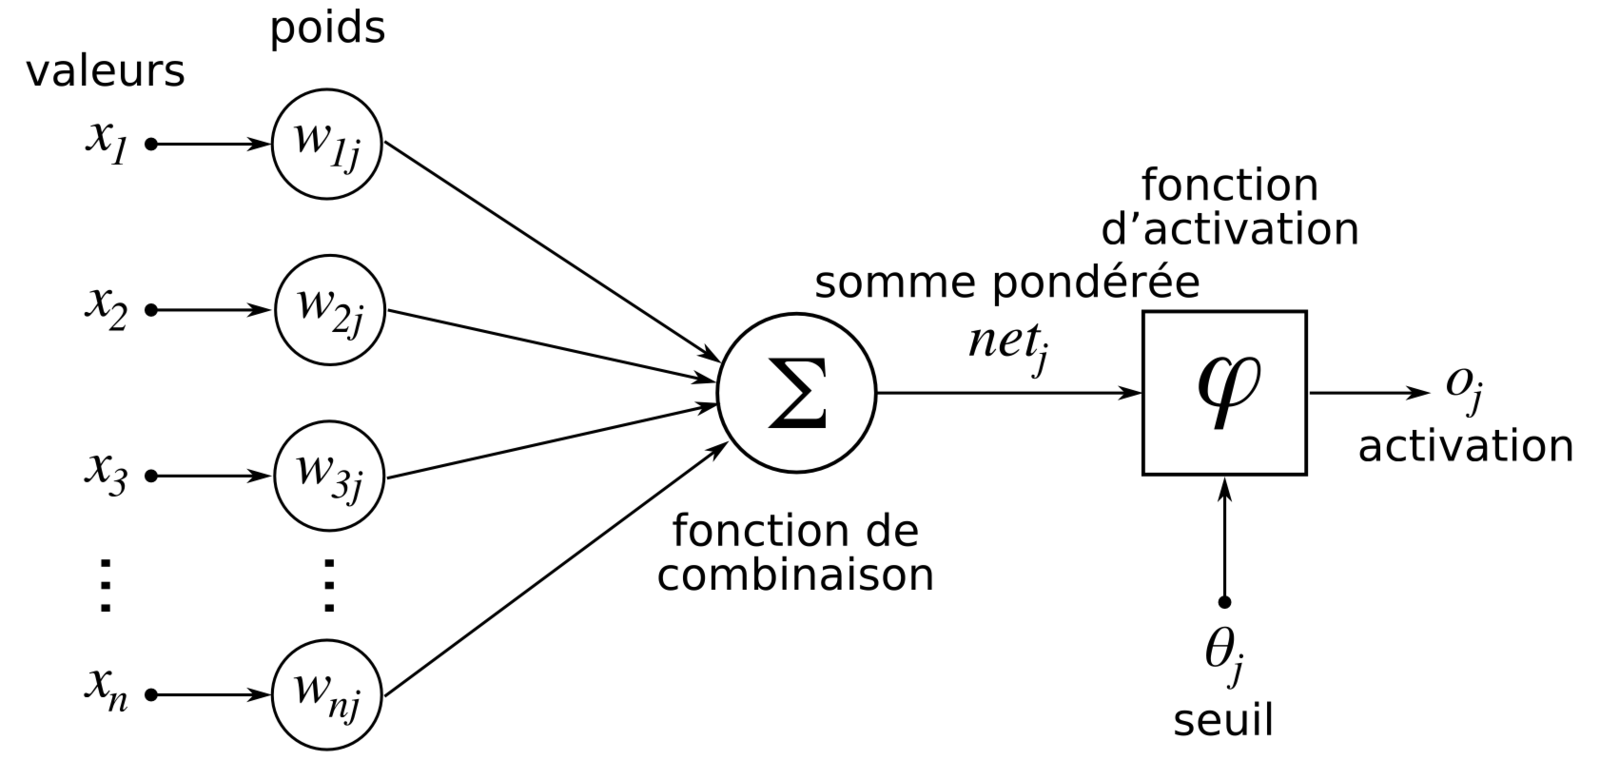
\includegraphics[width=10cm]{images_pfe/neurone.png}
	\caption{Le fonctionnement d'un neurone artificiel [\cite{mcculloch_pitts_1943_nervous_activity}].}
	\label{fig:fonctionnement-neurone}
\end{figure}
\FloatBarrier
\medskip

La fonction d'activation est utilisée pour introduire de la non-linéarité dans
le modèle, permettant ainsi de modéliser des relations complexes entre les
données d'entrée et de sortie [\cite{Goodfellow-et-al-2016}]. Les propriétés
d’une fonction d’activation doivent être vérifiées dans un problème
d'apprentissage profond. Ces propriétés sont:
\begin{itemize}
	\item \textbf{Non-linéarité}: lorsque la fonction d’activation est non linéaire, il est possible de prouver qu’un réseau neuronal à deux couches peut approximer n'importe quelle fonction continue sur un domaine compact à une précision arbitraire, ce que l’on appelle le \textbf{théorème d’approximation universelle} [\cite{Goodfellow-et-al-2016}].
	\item \textbf{L’intervalle}: lorsque l’intervalle des valeurs est fini, l'apprentissage de manière générale est plus efficace.
	\item \textbf{Différentiabilité}: cette propriété est importante quand les méthodes d’optimisation sont basées sur le gradient, car elles cherchent à optimiser l’apprentissage en se basant sur la  différentiabilité de la fonction.
	\item \textbf{Monotonie}: Une fonction d'activation est monotone si sa sortie augmente (ou diminue) à mesure que son entrée augmente. Cela garantit que le gradient de la fonction est toujours positif ou négatif, simplifiant ainsi l’apprentissage.
	\item \textbf{Efficacité en termes de calcul}: les fonctions d'activation doivent être efficaces en termes de calcul, afin que le réseau puisse être utilisé dans des applications en temps réel, sans ralentir le processus de l’apprentissage.
\end{itemize}
\medskip
Parmi les fonctions d'activation les plus couramment utilisées dans les réseaux de neurones, on peut citer:
\begin{itemize}
	\item \textbf{La fonction Sigmoïde}: si la probabilité d’un résultat est comprise entre 0 et 1, la fonction sigmoïde est le meilleur choix. Cette fonction est largement utilisée grâce à son intervalle et sa différentiabilité.
	      \begin{equation}
		      \sigma(x) = \frac{1}{1 + e^{-x}}
	      \end{equation}
	\item \textbf{La fonction Unité linéaire rectifiée (ReLU)}: c'est une fonction qui possède une dérivée et permet la rétropropagation (backpropagation) tout en étant efficace sur le plan informatique. Cependant, elle n’active pas les neurones en même temps, et c’est considéré comme désavantage pour cette fonction.
	      \begin{equation}
		      ReLU(x) = \max(0,x)
	      \end{equation}
	\item \textbf{La fonction Tangente hyperbolique (Tanh)}: cette fonction est très identique à la fonction d’activation sigmoïde. Sa plage de sortie est comprise entre -1 et 1. Avec cette fonction, plus l’entrée est grande, plus la valeur de sortie sera proche de 1, et plus l’entrée est petite, plus la sortie sera proche de -1.
	      \begin{equation}
		      tanh(x) = \frac{e^x - e^{-x}}{e^x + e^{-x}}
	      \end{equation}
\end{itemize}
\medskip
\begin{figure}[hbt!]
	\centering
	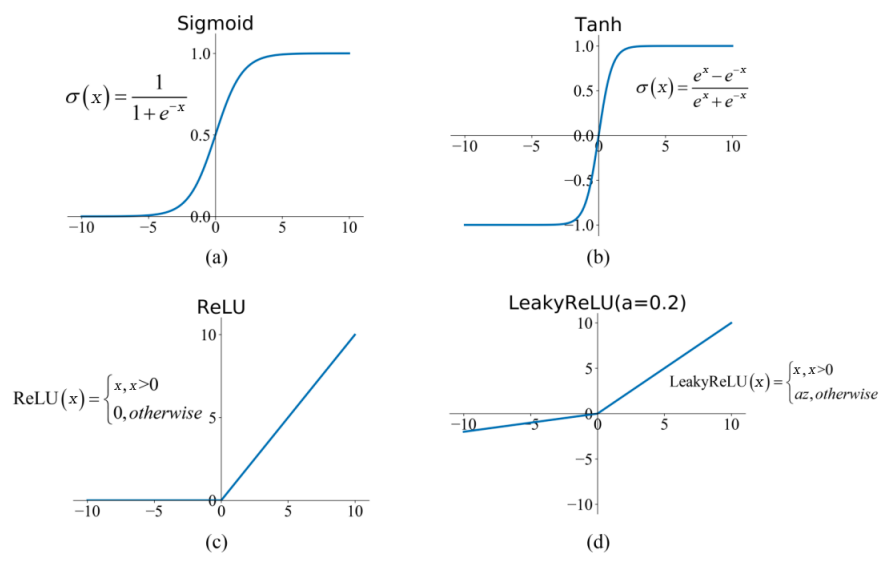
\includegraphics[width=12cm]{images_pfe/functions.png}
	\caption{Les fonctions d'activations couramment utilisées [\cite{feng_he_teng_ren_chen_li_2019}].}
	\label{fig:vue-snoc-pos}
\end{figure}
\FloatBarrier

\section{Couches dans un réseau de neurones}
Une couche (\textit{layer} en anglais) est une succession verticale des
neurones. Mathématiquement, elle est vue comme une composition de deux
fonctions \textit{h} et \textit{g} où \textit{g} est une fonction linéaire et
\textit{h} une fonction d’activation non linéaire. Cette composition de
fonction est définie par l'équation \ref{equ:couche}
[\cite{Goodfellow-et-al-2016}].

\begin{equation}
	y = h(g(x) + b)
	\label{equ:couche}
\end{equation}

\medskip
Une couche intermédiaire est donc l’ensemble des nœuds verticaux qui sont connectés à la couche précédente et à la couche suivante. La connectivité entre les couches détermine la manière dont les informations circulent sur le réseau. La façon de connexions des nœuds entre eux est différente d’une architecture à une autre [\cite{Goodfellow-et-al-2016}], et c’est ce qui détermine le type d'une couche:
\begin{itemize}
	\item \textbf{Couche entièrement connectée}: tous les neurones d'une couche sont connectés à tous les neurones de la couche suivante.
	\item \textbf{Couche partiellement connectée}: certains neurones ne sont pas connectés aux neurones de la couche suivante.
\end{itemize}

Les couches sont le composant principal des réseaux de neurones. Elles ont
plusieurs caractéristiques qui définissent leur comportement et influencent les
performances globales du réseau. Ces caractéristique sont les suivants:

\begin{itemize}
	\item \textbf{La matrice de poids}: Dans une couche d'un réseau de neurones, la matrice de poids est une matrice de paramètres qui représente les connexions entre les neurones d'entrée et les neurones de sortie de cette couche [\cite{aggarwal_2018}]. Elle définie la puissance des connexions entre les neurones des différentes couches. Chaque ligne de la matrice correspond aux poids associés à un neurone d'entrée particulier, et chaque colonne correspond aux poids associés à un neurone de sortie particulier,La taille de la matrice de poids dépend du nombre de neurones d'entrée et du nombre de neurones de sortie dans la couche.

	      La forme générale de la matrice de poids dans un réseau de neurones peut être
	      exprimée comme suit:
	      \begin{equation}
		      W = \begin{bmatrix}
			      w_{1,1} & w_{1,2} & ... & w_{1, m} \\
			      w_{2,1} & w_{2,2} & ... & w_{2, m} \\
			      ...     & ...     & ... & ...      \\
			      w_{n,1} & w_{n,2} & ... & w_{n, m}
		      \end{bmatrix}
	      \end{equation}

	      où $w_{i,j}$ représente le poids de la connexion entre le neurone \textit{i} de
	      la couche actuelle et le neurone \textit{j} de la couche suivante et
	      \textit{(n, m)} représente la dimension de la matrice.

	      La matrice de poids est crucial pour la performance du réseau neuronal,
	      puisqu'elle détermine la capacité du réseau d'apprendre et généraliser les
	      motifs a partir des données en entrées.

	\item \textbf{Type de couche}: Les couches forment les blocs de construction de base des réseaux de neurones. Elle permettent d'effectuer des calculs complexes et d'apprendre des relations qui existent entre données d'entrée et de sortie. Dans le réseau neuronal, il existe trois types de couches différents:
	      \begin{itemize}
		      \item \textbf{Couche d'entrée}: Cette couche est responsable de la réception des données d'entrée et de leur transmission à la couche suivante (la première couche parmi les couches cachées).
		      \item \textbf{Couche cachée}: Cette couche traite les entrées de la couche précédente et génère des valeurs de sortie qui sont transmises à la couche suivante. Les réseaux de neurones peuvent avoir plusieurs couches cachées, chacune effectuant différentes opérations sur les entrées.
		      \item \textbf{Couche de sortie}: Cette couche produit la sortie finale du réseau de neurones, qui peut être une classification, une régression ou un autre type de prédiction.
	      \end{itemize}
\end{itemize}

\medskip

\begin{figure}[hbt!]
	\centering
	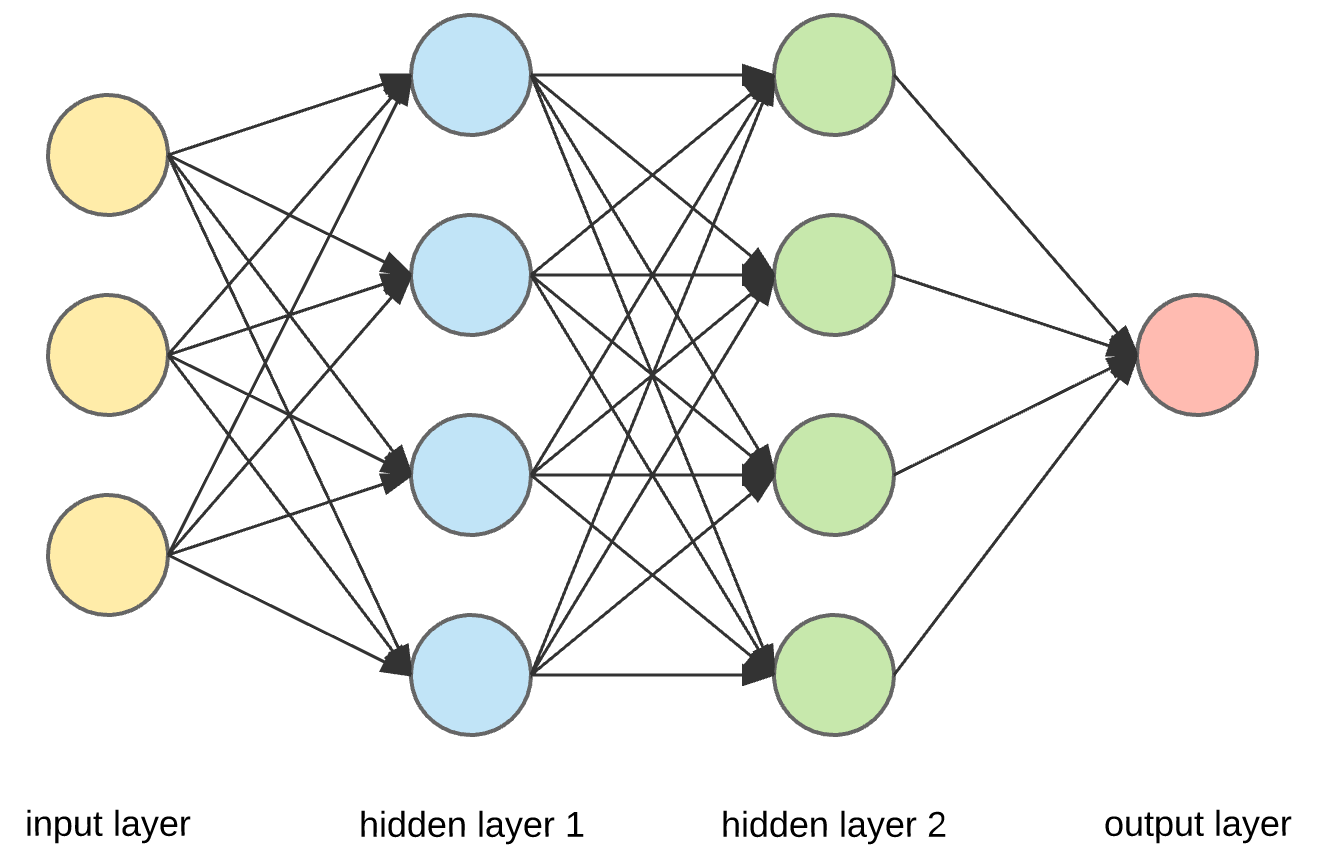
\includegraphics[width=12cm]{images_pfe/network.png}
	\caption{Schéma simple d'un réseau de neurones feedforward [\cite{dl-healthcare}].}
	\label{fig:schema-reseau}
\end{figure}
\FloatBarrier
\medskip

\section{Types de réseaux de neurones}
Dans l'apprentissage profond, il existe plusieurs classes de réseaux de
neurones, chacune avec sa propre architecture, caractéristiques, algorithme
d'apprentissage et application. Dans cette section, nous allons présenter les
différentes architecture de réseaux de neurones.
\subsection{Réseaux feedforward}
Les réseaux feedforward (ou réseaux entièrement connectés) sont un des types de
réseau de neurones artificiels où les informations circulent dans une seule
direction, de l'entrée vers la la sortie [\cite{Goodfellow-et-al-2016}]. Ils
sont composés d'une succession de couches interconnectées, où chaque neurone
d'une couche est connecté aux neurones de la couche suivante. Dans un Réseau de
ce type, les données sont introduites dans la première couche du réseau (couche
d'entrée), puis elles traversent plusieurs couches cachées avant d'atteindre la
couche de sortie (\textit{la figure \ref{fig:schema-reseau} est un schéma
	simple d'un réseau feedforward}).

Les réseaux feedforward sont indépendants de la structure, c’est-à-dire il
n’existe pas d’hypothèses particulières à faire sur l’entrée, ce qui les rend
largement applicables. Cependant, ils ont tendance à être moins performants que
les réseaux à usage spécial. Les réseaux feedforward sont couramment utilisés
dans les applications d'apprentissage supervisé. Ils peuvent également être
utilisés dans des applications d'apprentissage non supervisé
[\cite{aggarwal_2018}].

\medskip

\subsection{Réseaux de neurones récurrents (RNN)}
Les réseaux de neurones récurrents (RNN) sont des architectures conçus pour
fonctionner avec des données séquentielles, telles que: la reconnaissance de la
parole, la reconnaissance de la voie, l'analyse de séries chronologiques et le
traitement du langage naturel [\cite{Goodfellow-et-al-2016}]. Les principales
caractéristiques des RNN sont:
\begin{itemize}
	\item \textbf{Connexions récurrentes} : Les connexions dans les réseaux récurrents sont des connexions récurrentes qui permettent à l'information de persister au fil du temps. Cela signifie que la sortie du réseau à un pas de temps est réinjectée en entrée du réseau au pas de temps suivant.
	\item \textbf{État caché} : Les réseaux RNN maintiennent un état caché qui représente la mémoire du réseau. Cet état est mis à jour à chaque pas de temps en fonction de l'entrée courante et de l'état caché précédent.
	\item \textbf{RNN bidirectionnels} : Les réseaux RNN bidirectionnels traitent la séquence d'entrée dans les sens avant et arrière, ce qui permet de capturer le contexte des pas de temps passés et futurs.
\end{itemize}

\begin{figure}[hbt!]
	\centering
	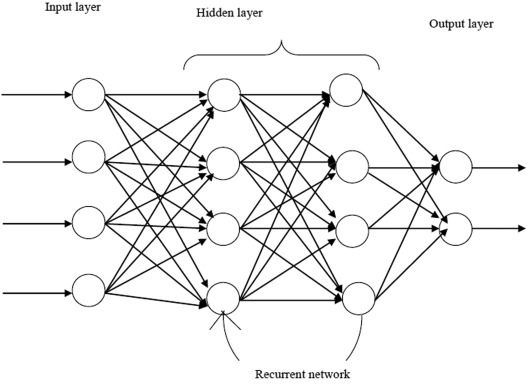
\includegraphics[width=12cm]{images_pfe/rnn.jpg}
	\caption{Exemple d'un réseau de neurones récurrent [\cite{kumaraswamy_2021}].}
	\label{fig:schema-reseau}
\end{figure}
\FloatBarrier

La capacité à conserver une mémoire des pas de temps précédents et à gérer les
dépendances à long terme rend les réseaux récurrents utiles pour les tâches qui
nécessitent de comprendre le contexte de la séquence d'entrée.

\subsubsection{Réseaux récurrents à mémoire courtet long terme (LSTM) }

Les réseaux de neurones récurrents à mémoire longue à court terme, ou Long
Short-Term Memory (LSTM) en angalis , représentent une amélioration
significative des réseaux de neurones récurrents traditionnels, conçue pour
résoudre les problèmes d’évanouissement et d’explosion du gradient. Introduits
par Hochreiter et Schmidhuber en 1997 dans [\cite{hochreiter1997long}], les
réseaux LSTM intègrent des cellules mémoire capables

de stocker et de conserver des informations tout au long du traitement d’une
séquence. Ces cellules mémoire permettent de transporter des informations
importantes grâce à trois types de portes : la porte d’entrée, la porte de
sortie et la porte d’oubli. Ces portes jouent un rôle crucial en décidant
quelles informations doivent être ajoutées, conservées ou oubliées.

\textbf{Porte d'Entrée}: décide quelles nouvelles informations doivent être stockées dans la cellule de mémoire. Elle est définie par :

\begin{equation}
	i_t = \sigma(W_i \cdot [h_{t-1}, x_t] + b_i)
\end{equation}

où $\sigma$ représente la fonction sigmoïde, $W_i$ est le poids associé à la
porte d'entrée, $h_{t-1}$ est l'état caché précédent, $x_t$ est l'entrée
actuelle, et $b_i$ est le biais.

\textbf{Porte d'Oubli}: contrôle quelles informations anciennes doivent être effacées de la cellule de mémoire. Elle est définie par :

\begin{equation}
	f_t = \sigma(W_f \cdot [h_{t-1}, x_t] + b_f)
\end{equation}

où $\sigma$ est la fonction sigmoïde, $W_f$ est le poids associé à la porte
d'oubli, $h_{t-1}$ est l'état caché précédent, $x_t$ est l'entrée actuelle, et
$b_f$ est le biais.

\textbf{Porte de Sortie}: décide quelles informations de la cellule de mémoire sont utilisées pour calculer l'état caché actuel. Elle est définie par :

\begin{equation}
	o_t = \sigma(W_o \cdot [h_{t-1}, x_t] + b_o)
\end{equation}

où $\sigma$ est la fonction sigmoïde, $W_o$ est le poids associé à la porte de
sortie, $h_{t-1}$ est l'état caché précédent, $x_t$ est l'entrée actuelle, et
$b_o$ est le biais.

\begin{figure}[hbt!]
	\centering
	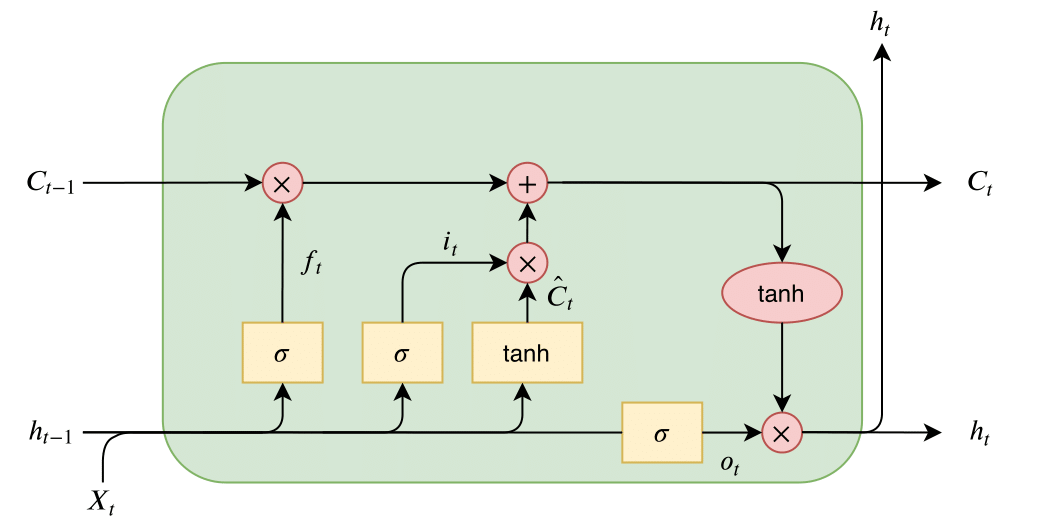
\includegraphics[width=15cm]{images_pfe/lstm.png}
	\caption{Architecture d'un bloc LSTM [\cite{fawaz2019long}].}
	\label{fig:lstm}
\end{figure}
\FloatBarrier
\medskip

\subsection{Réseaux de neurones convolutifs (CNN)}
L'architecture des réseaus de neurones convolutifs (CNN) est une architecture
spéciale qui est bien adaptée à la tâche de classification d'images. Ces
réseaux comportent trois types de couches: \textbf{convolutives},
\textbf{pooling} et \textbf{d'activation} [\cite{Goodfellow-et-al-2016}].

Les couches convolutives sont appliquées à l'image en entrée pour l’extraction
des caractéristiques importantes de l'image. Ensuite, ces dernières traversent
des couches d'activation, qui sont responsables de l'application d'une fonction
d'activation non-linéaire à ces caractéristiques. Les couches d'activation sont
suivies de couches de pooling qui réduisent la taille de l'image. Les couches
de pooling sont elles même suivies par une couche entièrement connectée qui
donne la classification de l'image (la sortie finale du modèle)
[\cite{Goodfellow-et-al-2016}].

\begin{figure}[hbt!]
	\centering
	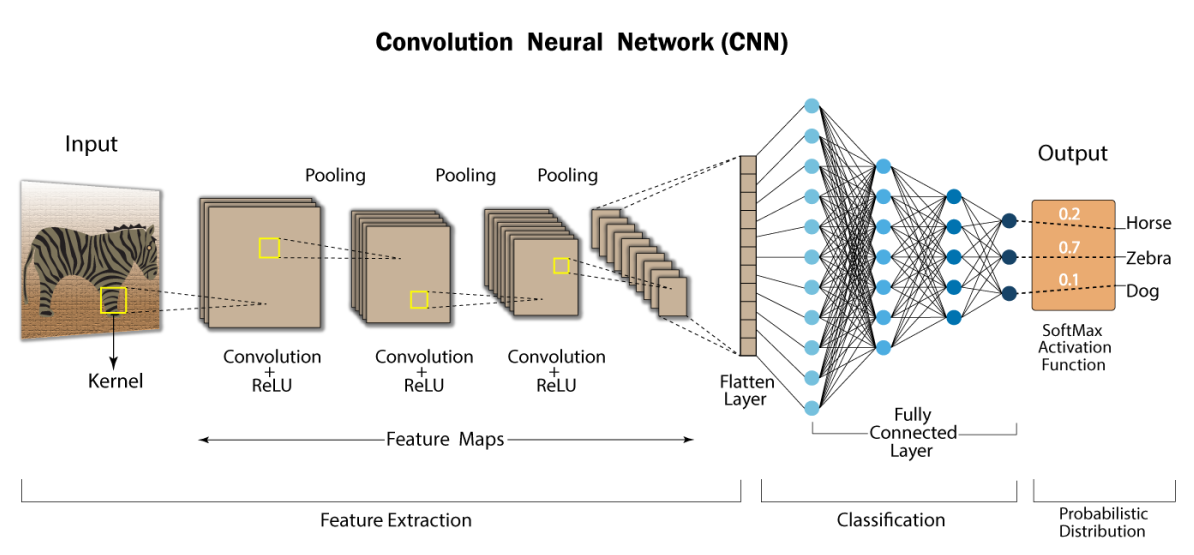
\includegraphics[width=15
		cm]{images_pfe/cnn.png}
	\caption{Le fonctionnement d'un réseau neuronal convolutif [\cite{alharbi_hewahi_2021}].}
	\label{fig:cnn}
\end{figure}
\FloatBarrier
\medskip

\subsubsection{Couche convolutive }
Une couche convolutive est un élément constitutif des réseaux de neurones
convolutifs (CNN). Elle est utilisé pour extraire des caractéristiques à partir
de données d'entrée, souvent des images, en appliquant un ensemble de filtres
convolutifs appris à l'entrée.

\medskip
Dans une couche convolutive, chaque filtre est convolué avec l'entrée pour produire une carte de caractéristiques. Cette opération est faite en glissant le filtre sur l'entrée et en calculant le produit scalaire à chaque position. Généralement, une couche convolutive possède trois hyperparamètres qui doivent être définis : \textbf{le nombre de filtres}, \textbf{la taille des filtres} et \textbf{la Stride}. Le nombre de filtres détermine le nombre de cartes d'entités produites, tandis que la taille des filtres détermine la taille du champ récepteur de chaque carte d'entités. La stride détermine la quantité de décalage du filtre à chaque étape.

\medskip
Les couches convolutives sont suivies de fonctions d'activation,et de couches de pooling. Ces dernières permettent de réduire les dimensions spatiales des cartes d'entités. Plusieurs couches convolutives peuvent être empilées pour créer un réseau neuronal convolutif profond.Les couches convolutives sont particulièrement efficaces pour traiter des images et d'autres données de grande dimension avec une structure spatiale, car elles peuvent apprendre automatiquement à détecter les caractéristiques importantes, telles que les bords, les coins et les textures [\cite{kimura_yoshinaga_sekijima_azechi_baba_2019}, \cite{Goodfellow-et-al-2016}].

\begin{figure}[hbt!]
	\centering
	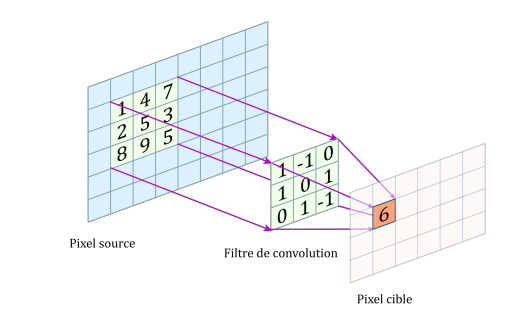
\includegraphics[width=12
		cm]{images_pfe/layerconv.png}
	\caption{Exemple du fonctionnement d'une couche convolutive [\cite{kimura_yoshinaga_sekijima_azechi_baba_2019}].}
	\label{fig:conv}
\end{figure}
\FloatBarrier
\medskip

\subsubsection{Couche pooling}
Le pooling est une opération quie est utilisée pour sous-échantillonner les
cartes de caractéristiques résultantes des couches convolutives en réduisant
leurs dimensions spatiales tout en conservant les informations importantes.
Parmi les types de pooling, on trouve le pooling maximal et le pooling moyen
	[\cite{Goodfellow-et-al-2016}].

\medskip
Dans le pooling maximal, la valeur maximale de chaque région est sélectionnée comme valeur représentative, tandis que dans le pooling moyen, la valeur moyenne est calculée à la place. Il en résulte une carte d'entités plus petite avec une résolution spatiale réduite, qui peut être traitée plus efficacement par les couches suivantes du réseau.

\medskip
Cependant, le pooling excessive peut entraîner une perte d'informations spatiales importantes. Il est donc important d'équilibrer la quantité de pooling avec les besoins du réseau et la nature de la tâche à accomplir.

\begin{figure}[hbt!]
	\centering
	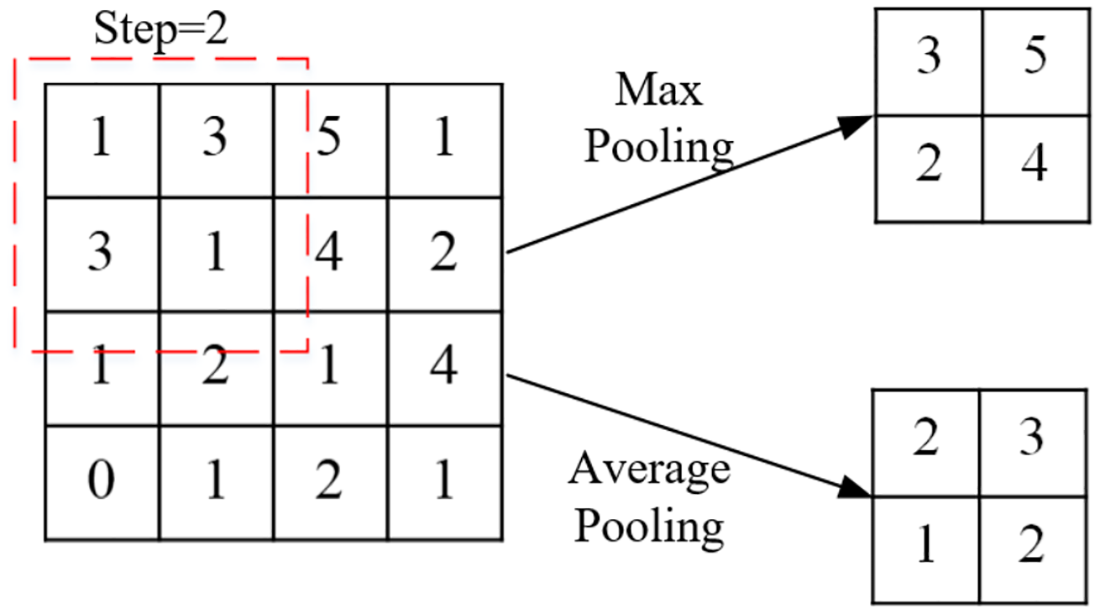
\includegraphics[width=9cm]{images_pfe/pooling.png}
	\caption{Exemples de pooling maximal et pooling moyen [\cite{hu_wu_xu_lai_xia_2022}].}
	\label{fig:pooling}
\end{figure}
\FloatBarrier
\medskip

\subsection{Réseaux résiduels (ResNet)}
Les réseaux résiduels ont été conçus par Microsoft afin de résoudre le problème
des gradients qui disparaissent dans les réseaux de neurones très profonds, ce
qui peut rendre l'entraînement difficile et diminuer significativement les
performances du réseau.

\medskip
Un ResNet est composé d'une ensemble de blocs résiduels, qui sont constitués de plusieurs couches avec des connexions de raccourci qui contournent une ou plusieurs couches. Ces raccourcis permettent aux gradients de circuler plus facilement à travers le réseau et évitent qu'ils ne disparaissent à mesure que le réseau devient plus profond [\cite{He_2016_CVPR}].

\begin{figure}[hbt!]
	\centering
	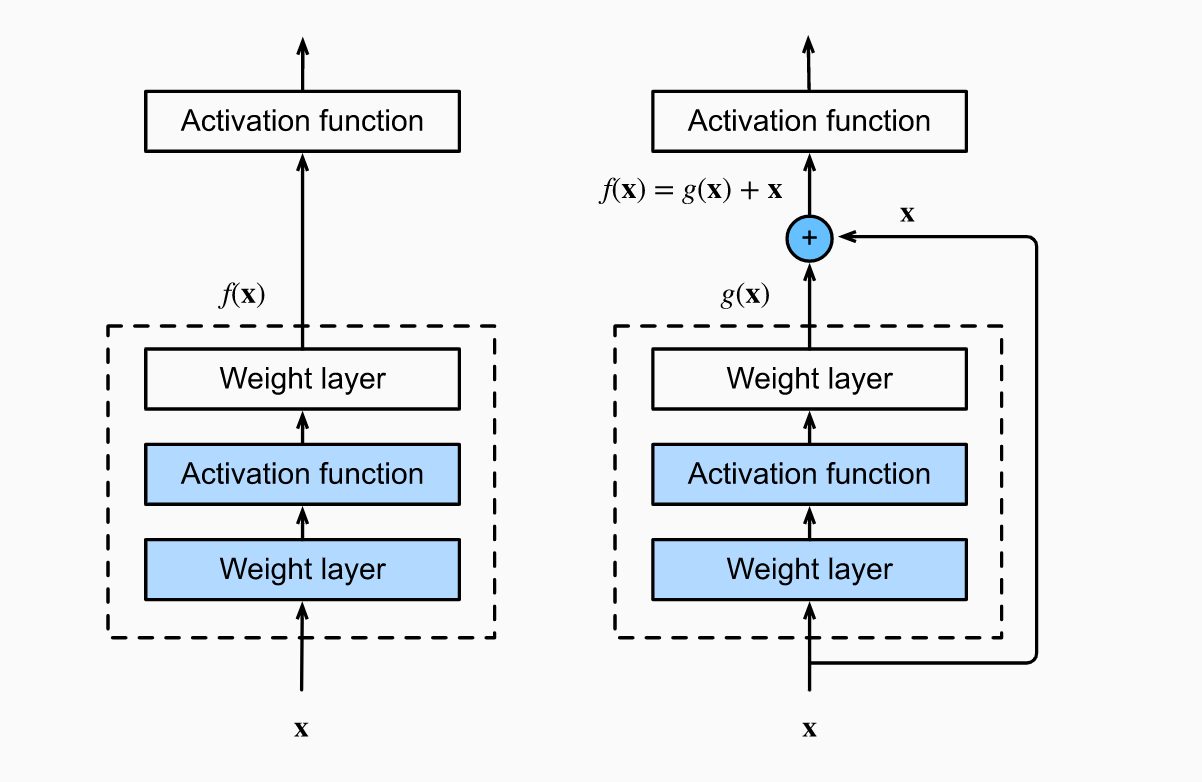
\includegraphics[width=12cm]{images_pfe/residual-net.png}
	\caption{Un bloc régulier (gauche) et un bloc résiduel (droite) [\cite{dong_niu_li_xie_zou_ye_wei_pan_2022}].}
	\label{fig:residual-net}
\end{figure}
\FloatBarrier

\medskip
ResNet est très efficace dans les tâches de vision par ordinateur, telles que la classification d'images, la détection d'objets et la segmentation. Il a joué un rôle important dans l'avancement de l'état de l'art en apprentissage profond et en vision par ordinateur, et continue d'être un domaine de recherche actif.

\subsection{Réseaux de neurones en graphe (GNN)}
Les réseaux de neurones en graphe (GNN) sont conçus pour traiter des données
structurées sous forme de graphes. Les GNN sont capables d'apprendre et de
faire des prédictions sur les données du graphe en propageant les informations
à travers les bords et les nœuds du graphe [\cite{ZHOU202057}].

\medskip
L'idée de base derrière les GNN est d'utiliser un ensemble de paramètres entraînables pour transformer les caractéristiques de chaque nœud dans le graphe en fonction des caractéristiques de ses nœuds voisins (plongement de graphe). Ce processus est répété de manière itérative sur plusieurs couches du réseau, permettant au GNN d'apprendre des motifs et des relations complexes à partir des données [\cite{ZHOU202057}].

\medskip
Parmi les tâches réalisées par ce type de réseaux:
\begin{itemize}
	\item \textbf{Classification des graphes} : Les GNN peuvent être utilisées pour classer des graphes en différentes catégories, tels que dans le cas de l'analyse des réseaux sociaux, la classification de textes et classification des molécules.
	\item \textbf{Prédiction de lien} : Les GNN peuvent prédire le lien manquant entre une paire de nœuds dans un graphe avec une matrice d'adjacence incomplète. Ils sont souvent utilisés pour les réseaux sociaux (tel que la suggestion des amis)
	\item \textbf{Plongement de graphe} : Les GNN permettent de faire la transformation de graphe en vecteurs, en préservant les informations pertinentes sur les nœuds, les arêtes et la structure générale du graphe.
\end{itemize}

\begin{figure}[hbt!]
	\centering
	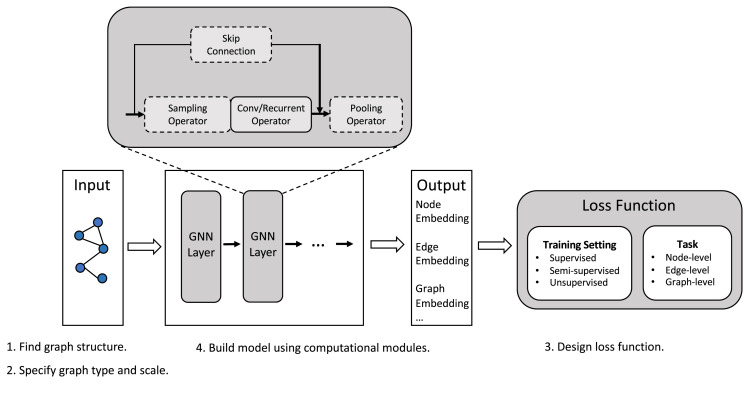
\includegraphics[width=15cm]{images_pfe/gnn.jpg}
	\caption{Le pipeline de conception générale pour un modèle GNN [\cite{ZHOU202057}].}
	\label{fig:gnn}
\end{figure}
\FloatBarrier
\medskip

\section{Le processus d’apprentissage}
L’apprentissage est le processus itératif et continu d’ajustement des
paramètres du réseau neuronal afin d’obtenir une meilleure précision du modèle
[\cite{Goodfellow-et-al-2016}]. Il peut être complexe car il nécessite souvent
une combinaison de techniques telles que le \textbf{prétraitement} des données,
le choix de l'architecture du réseau de neurones et des hyperparamètres, ainsi
que l'algorithme d'optimisation.

Ce processus d'apprentissage commence d'abord par l'initialisation aléatoire
des paramètres (poids) du modèle. Ensuite, le modèle est entraîné sur un
ensemble de données (\textbf{dataset}) en utilisant un algorithme
d'optimisation pour ajuster les poids du modèle afin de minimiser la perte.

Lors de l'entraînement, le modèle est alimenté en entrée avec des exemples à
partir du dataset d'entrainement et compare sa sortie à la sortie attendue.
Ensuite, il calcul la perte en faisant la différence entre la sortie prédite et
la sortie attendue. L'algorithme de \textbf{rétropropagation} de gradient
ajuste les poids du modèle en claculant les gradient de la fonction de perte
afin de la minimiser.

Le processus d'apprentissage continue jusqu'à ce que la performance du modèle
sur le dataset de validation arrête de s'améliorer ou jusqu'à ce qu'un nombre
prédéfini d'itérations d'apprentissage soit atteint. Le modèle final est
ensuite utilisé pour effectuer des prédictions sur de nouvelles données.

\medskip
Ce processus peut être résumé dans les points suivants:
\begin{itemize}
	\item L’apprentissage consiste à modifier progressivement les paramètres (poids) en
	      passant un lot de données en entrée et en évaluant le taux de perte.
	\item La définition de la fonction de perte est utilisée pour les modifications de
	      réseaux dans le processus de l'entraînement.
	\item La modification des poids du réseau est effectuée grâce a l’algorithme de
	      rétropropagation (backpropagation).
\end{itemize}

\subsection{Descente de gradient}
La descente de gradient est une méthode utilisée dans le processus
d’optimisation. Elle est basée sur la différentiabilité d’une fonction et elle
est appliquée pour calculer la fonction dérivée du premier ordre pour trouver
le minimum de la fonction de perte [\cite{Goodfellow-et-al-2016}]. Sa
simplicité d’application est l’un des avantages de cette méthode.

L'algorithme commence par l'initialisation aléatoire des paramètres (poids) du
modèle. Ensuite, il calcule le gradient de la fonction de perte par rapport à
chaque paramètre. Le gradient indique la direction dans laquelle la fonction de
perte augmente le plus, donc l'algorithme met à jour les paramètres dans la
direction opposée au gradient pour réduire la valeur de perte. Ce processus est
répété itérativement jusqu'à ce que la valeur de perte ne puisse plus être
réduite ou jusqu'à ce qu'un critère d'arrêt soit atteint. Le taux
d'apprentissage est un hyperparamètre qui contrôle la taille des mises à jour
de paramètres et la vitesse de convergence de l'algorithme
[\cite{Goodfellow-et-al-2016}].

Des variantes de la descente de gradient existent, telles que la descente de
gradient stochastique, Adam et la descente de gradient avec moment.

\subsection{Propagation de l’erreur}
La propagation d'erreur est utilisée dans le processus d'apprentissage pour
calculer le gradient de la fonction de perte par rapport aux paramètres du
modèle [\cite{Goodfellow-et-al-2016}].

Dans la propagation d'erreur, l'erreur est propagée en arrière à travers les
couches du modèle, en commençant par la couche de sortie et en allant vers
l'entrée. Chaque couche calcule la dérivée de sa sortie par rapport à ses
entrées, qui est ensuite multipliée par l'erreur propagée de la couche
suivante. Ce processus est répété jusqu'à ce que l'erreur soit propagée jusqu'à
la couche d'entrée, où le gradient de la fonction de perte par rapport aux
paramètres du modèle est obtenu [\cite{Goodfellow-et-al-2016}].

\begin{figure}[hbt!]
	\centering
	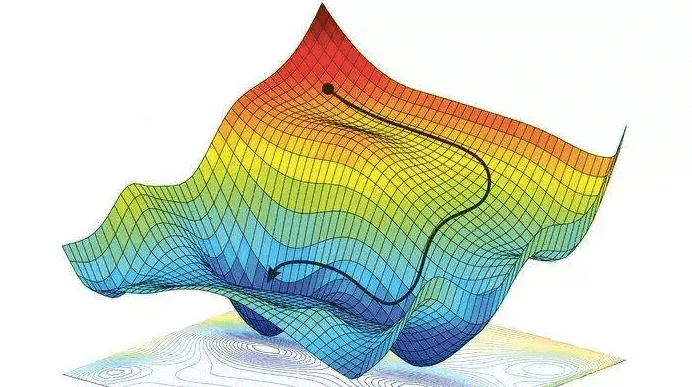
\includegraphics[width=10cm]{images_pfe/gd.png}
	\caption{Fonction de taux d’erreur [\cite{amini2018spatial}].}
	\label{fig:error-function}
\end{figure}
\FloatBarrier
\medskip

\subsection{Hyperparameters}
Les hyperparamètres sont les paramètres qui sont définis avant de lancer le
processus d'apprentissage et ils contrôlent l'entraînement. Les valeurs des
hyperparamètres, contrairement aux paramètres du modèle, ne sont pas apprises
lors de l'apprentissage [\cite{Goodfellow-et-al-2016}]. Parmi les
hyperparamètres, on peut définir:
\begin{itemize}
	\item \textbf{Taux d'apprentissage} : Il contrôle la vitesse d'apprentissage du modèle à partir des données.
	\item \textbf{Nombre d'époques} : Le nombre d'époques correspond au nombre d'itération sur le dataset d'entraînement.
	\item \textbf{Taille du batch} : Elle représente le nombre d'échantillons des données d'entraînement qui sont utilisés dans un passage avant/arrière (feedforward et backpropagation).
	\item \textbf{Nombre de couches} : C'est un hyperparamètre qui caractérise la profondeur du réseau.
	\item \textbf{Fonction d'activation} : La fonction d'activation est utilisée pour introduire la non-linéarité dans le modèle. C'est un hyperparamètre qui contrôle la sortie du neurone.
	\item \textbf{Initialisation des poids} : Les valeurs initiales des poids peuvent affecter de manière significative les performances du modèle. Elle affecte le processus de trouver le minimum local ou le minimum global.
	\item \textbf{Paramètre de régularisation} : Il est utilisé pour éviter le \textbf{surapprentissage}, c'est-à-dire éviter de construire un modèle qui est trop complexe par rapport à la quantité de données d'entraînement. Cela peut entraîner une adaptation excessive du modèle aux données d'entraînement et une mauvaise généralisation aux données inconnues.
	\item \textbf{Optimiseur} : L'optimiseur est l'algorithme utilisé pour mettre à jour les poids pendant l'entraînement.
\end{itemize}

Cependant, le réglage de ces hyperparamètres peut être une tâche complexe
nécessitant souvent des essais et des erreurs.

\section{Types d’apprentissage}
Il existe plusieurs types d’apprentissage, et chacun de ces types a des
applications spécifiques en deep learning, et peut être utilisé pour résoudre
différents types de problèmes. Dans ce qui suit, nous parlons brièvement sur
les quatre types d'apprentissage en deep learning les plus courants:
l'apprentissage supervisé, l'apprentissage non supervisé, l'apprentissage
semi-supervisé et l'apprentissage par renforcement.

\subsection{Apprentissage supervisé}
Dans l'apprentissage supervisé, l'apprentissage s'effectue sur un ensemble de
données étiqueté, où les étiquettes sont connues à l'avance. En d'autres
termes, les données d'entrée sont accompagnées d'étiquettes de sortie ou de
valeurs cibles correspondantes. Le but de l'apprentissage supervisé est
d'apprendre à prédire les étiquettes à partir des données d'entrée, de sorte
que lorsqu'on donne au modèle de nouvelles données en entrée, l'algorithme
puisse prédire la sortie correspondante. Pendant le processus d'apprentissage,
l'algorithme ajuste itérativement ses paramètres pour minimiser la différence
entre la sortie prédite et la sortie réelle [\cite{aggarwal_2018},
\cite{Goodfellow-et-al-2016}].

\medskip
Ce type d'apprentissage est applicable dans plusieurs domaines, tels que la reconnaissance d'images et de la parole, le traitement du langage naturel et la modélisation prédictive dans la finance, la santé, le marketing, etc. Parmi les algorithmes d'apprentissage supervisés, nous pouvons citer la régression linéaire et les arbres de décision.

\subsection{Apprentissage non-supervisé}
L'apprentissage non supervisé se fait sur un dataset non étiqueté, sans aucune
information sur les étiquettes [\cite{Goodfellow-et-al-2016}]. En d'autres
termes, il n'y a pas de valeurs cibles ou d'étiquettes de sortie fournies à
l'algorithme. L'algorithme est laissé à lui-même pour trouver les motifs et
relations dans les données, sans recevoir d'instructions explicites sur ce
qu'il faut rechercher.

\medskip
L'utilisation de cette approche d'apprentissage peut impliquer le regroupement de points de données similaires, la découverte de structures ou de caractéristiques cachées dans les données (réduction de la dimensionnalité) ou l'identification de valeurs aberrantes ou d'anomalies dans les données.

\medskip
Nous pouvons appliquer l'apprentissage non supervisé dans divers domaines, tels que la segmentation des marchés, la détection d'anomalies et l'extraction de caractéristiques. Parmi les algorithmes d'apprentissage non supervisés courants, on trouve le clustering k-means, l'analyse en composantes principales (PCA) et les auto-encodeurs.

\medskip
L'un des principaux défis dans l'apprentissage non supervisé est d'évaluer la qualité des résultats, car il n'y a pas d'objectifs ou d'étiquettes explicites à comparer. Au lieu de cela, les résultats sont souvent évalués en fonction de leur utilité ou de leur interprétabilité pour une tâche ou un domaine particulier.

\subsection{Apprentissage semi-supervisé}
L'apprentissage semi-supervisé est un type d'apprentissage qui combine des
éléments d'apprentissage supervisé et non supervisé. Dans l'apprentissage
semi-supervisé, un petit ensemble de données étiquetées est fourni, tandis que
la grande partie de données est non étiquetées [\cite{Goodfellow-et-al-2016}].

\medskip
Le but dans l'apprentissage semi-supervisé est d'utiliser les données étiquetées pour guider le processus d'apprentissage sur les données non étiquetées, afin d'améliorer la précision du modèle. Cela peut être particulièrement utile dans les situations où il est difficile ou coûteux d'obtenir des données étiquetées, mais il existe une abondance de données non étiquetées disponibles.

\medskip
Il existe plusieurs approches, mais une méthode courante consiste à utiliser les données étiquetées pour créer un modèle, puis à utiliser ce modèle pour faire des prédictions sur les données non étiquetées. Les étiquettes prédites sont ensuite utilisées pour améliorer le modèle, et le processus est répété de manière itérative.

\medskip
L'un des défis de l'apprentissage semi-supervisé est que la qualité des résultats peut dépendre fortement de la distribution des données non étiquetées. Si les données non étiquetées ne sont pas représentatives du domaine cible, le modèle peut mal fonctionner même avec une grande quantité de données non étiquetées.

\subsection{Apprentissage par renforcement}
L'apprentissage par renforcement se concentre sur la prise de décision. Il
s'agit d'une méthode d'apprentissage dans laquelle un agent apprend à prendre
des décisions en interagissant avec un environnement. L'agent doit choisir une
action à partir d'un état donné, et l'environnement renvoie un signal de
récompense ou de pénalité en fonction de l'action choisie. L'objectif de
l'agent est de maximiser la récompense totale sur une période donnée
[\cite{wiering2012reinforcement}]. Dans le chapitre suivant, nous présenterons
l'apprentissage par renforcement et nous en parlerons avec plus de détails.

\section{Catégories de données}
La division du jeu de données est une étape cruciale avant de commencer
l'entraînement du modèle de manière. Elle permet d'éviter les problèmes de
surapprentissage. Il est courant de diviser un jeu de données en trois parties
distinctes: l'ensemble d'entraînement, l'ensemble de validation et l'ensemble
de test [\cite{Goodfellow-et-al-2016}].

\begin{itemize}
	\item \textbf{Ensemble d'entraînement}: Il s'agit de la partie de données utilisée pour entraîner le modèle. Il est important que ce dataset soit représentatif de l'ensemble des données et qu'il contienne une variété de cas d'utilisation différents.

	\item \textbf{Ensemble de validation}: Il s'agit d'un sous-ensemble de l'ensemble de données utilisé pour évaluer les performances du modèle pendant l'entraînement. L'ensemble de validation est utilisé pour régler les hyperparamètres du modèle et pour éviter le surapprentissage. Il est important qu'il soit représentatif et distinct du dataset d'entraînement.

	\item \textbf{Ensemble de test}: Il s'agit d'un ensemble de données utilisé pour évaluer les performances du modèle après son entraînement. L'ensemble de test est utilisé pour obtenir une estimation impartiale de la performance du modèle sur de nouvelles données inédites, donc il est nécessaire que ce dataset soit représentatif de l'ensemble des données et distinct des deux autres datasets cités précédemment.
\end{itemize}
La distinctivité des datasets assure que le modèle se généralise bien aux nouvelles données invisibles. En règle générale, l'ensemble de données est divisé en ces trois ensembles dans un rapport de 60-20-20 ou 70-15-15 respectivement.

\section{Défis de l'apprentissage profond}
L'apprentissage profond a fait des progrès remarquables ces dernières années et
a obtenu des résultats excellents dans divers domaines tels que la vision par
ordinateur, le traitement du langage naturel et la reconnaissance de la parole.
Cependant, il reste encore plusieurs défis à relever afin d'améliorer encore
l'efficacité et l'efficience des modèles d'apprentissage profond. Certains
défis majeurs incluent:
\begin{itemize}
	\item \textbf{Rareté des données} : les modèles d'apprentissage profond nécessitent une grande quantité de données pour être entraînés efficacement. Cependant, dans de nombreux domaines, tels que l'imagerie médicale et la conduite autonome, les données sont rares et coûteuses à collecter.

	\item \textbf{Surapprentissage (overfitting)} : les modèles d'apprentissage profond peuvent facilement sur-adapter les données d'apprentissage, en particulier lorsque le modèle comporte un grand nombre de paramètres. Le surapprentissage peut entraîner de mauvaises performances de généralisation sur de nouvelles données.

	\item \textbf{Interprétabilité} : les modèles d'apprentissage profond sont souvent appelés "boîtes noires" car il peut être difficile de comprendre comment ils arrivent à leurs prédictions. Ce manque d'interprétabilité peut compliquer le débogage et l'amélioration des modèles de l’apprentissage profond

	\item \textbf{Limitations matérielles} : les modèles d'apprentissage profond  sont coûteux en termes de calcul et nécessitent un matériel spécialisé tel que des unités de traitement graphique (GPU) ou des unités de traitement de tenseur (TPU). Le coût de ce matériel peut constituer un obstacle pour les petits groupes de chercheurs ou les entreprises.

	\item \textbf{Attaques contradictoires} : les modèles d'apprentissage profond  peuvent être vulnérables aux attaques contradictoires, où un attaquant manipule délibérément les données d'entrée pour amener le modèle à faire des prédictions incorrectes.

\end{itemize}

\section{Conclusion}
En conclusion, l'apprentissage profond est devenu un domaine de recherche actif
de l'apprentissage automatique qui a révolutionné la façon dont nous abordons
de nombreux problèmes difficiles, tels que la vision par ordinateur, le
traitement du langage naturel et la robotique. Avec l'avènement d'un matériel
puissant, d'ensembles de données à grande échelle et d'algorithmes
sophistiqués, les modèles d'apprentissage profond ont connu un avancement
remarquable dans plusieurs domaines tels que la reconnaissance d'images, la
reconnaissance vocale, la traduction linguistique et la conduite autonome.

\medskip
Malgré son énorme succès, l'apprentissage en profondeur fait encore face à plusieurs défis, tels que le besoin d'algorithmes d'entraînement plus efficaces et fiables, une meilleure interprétabilité, etc. L’utilisation et l'entraînement de modèles d’apprentissage profond exigent des ordinateurs assez puissants et ne peuvent pas être utilisés sur les appareils moins puissants comme les ordinateur embarqués ou les smartphones, ce qui signifie qu'on a besoin de trouver des moyens pour optimisation ces modèles afin de les utiliser ultérieurement par les machines moins puissantes. Ces méthodes d'optimisation font l'objet du dernier chapitre.

\medskip
Dans ce qui suit, nous présenterons l'apprentissage profond et ses algorithmes. La raison pour laquelle on a réservé un chapitre complet pour l'apprentissage profond est que ce type d'apprentissage peut aider beaucoup dans l'optimisation des réseaux de neurones profonds, comme nous le verrons plus tard.

\clearpage

%%%%%%%%%%%%%%%%%%%%%%%%%%%%%% Intelligence artificielle générative (GenAI) %%%%%%%%%%%%%%%%%%%%%%%%%%%%%%%%%%%%%%%

\chapter{Intelligence Artificielle Générative (GenAI)}
\section{Introduction}

Avec les avancées fulgurantes du deep learning, de nouvelles méthodes
d'intelligence artificielle ont émergé, souvent désignées sous le terme de
modèles génératifs. Ces technologies de pointe, telles que les auto-encodeurs
variationnels, les réseaux adversariaux génératifs (GANs), les modèles de
diffusion, les transformers et les modèles de langage de grande taille (LLM)
sont capables de produire des données d'une qualité impressionnante,
ressemblant de manière frappante aux données réelles. Les données générées par
ces modèles sont souvent indiscernables des données authentiques, ce qui pose
de nouveaux défis en matière d'identification et d'authenticité.Les modèles
génératifs permettent la génération de textes, d'images, de séries temporelles
et de données tabulaires avec une grande précision.

\medskip

La puissance de ces modèles repose sur des ressources de calcul considérables,
notamment l'utilisation de GPU, et sur l'accès à des ensembles de données
massifs. Par exemple, des modèles tels que ChatGPT-4 ont été entraînés sur
l'intégralité du contenu disponible sur Internet.

\medskip

Dans ce chapitre, nous allons examiner en détail les différentes architectures
de ces modèles génératifs, ainsi que les techniques et pratiques associées à
leur fonctionnement et à leur mise en œuvre. Nous aborderons les principes de
base, les innovations récentes, et les applications potentielles de ces
technologies révolutionnaires.

\section{Les Auto-Encodeurs Variationnels (VAE)}
\subsection{Introduction}

Les auto-encodeurs variationnels (VAE) sont des modèles génératifs puissants,
reconnus pour leur capacité à apprendre une représentation compacte et
structurée des données. Cette approche a révolutionné le domaine de
l'apprentissage non supervisé et des modèles génératifs. Les VAE appartiennent
à la classe des modèles génératifs probabilistes, combinant les principes des
autoencodeurs et des modèles de variational Bayes pour générer des données
nouvelles et similaires à celles d'un jeu de données d'entraînement. Depuis
leur introduction par Kingma et Welling en 2013
	[\cite{kingma_welling_auto_encoding}] , les VAE ont connu un grand succès dans
diverses applications, allant de la génération d'images à la synthèse de texte.

\subsection{Fonctionnement}
Les VAE sont composés de trois éléments principaux : l'encodeur, le décodeur et
l'espace latent. Chacune de ces composantes joue un rôle crucial dans le
fonctionnement global du modèle.

\textbf{L'Encodeur:}L'encodeur est responsable de la transformation des données d'entrée \(\mathbf{x}\) en une distribution
dans l'espace latent. Plus précisément, il mappe les données d'entrée à une distribution gaussienne paramétrée par
une moyenne \(\mu\) et une variance \(\sigma^2\). Cette distribution est souvent représentée comme :

\begin{equation}
	q(\mathbf{z} \mid \mathbf{x}) = \mathcal{N}(\mathbf{z} \mid \mu(\mathbf{x}), \sigma^2(\mathbf{x}))
	\label{equ:couche}
\end{equation}

où \(\mathbf{z}\) est la variable latente que l'encodeur cherche à estimer.

\medskip

\textbf{Le Décodeur:}Le décodeur prend un échantillon \(\mathbf{z}\) de la distribution gaussienne dans
l'espace latent et génère une reconstruction \(\hat{\mathbf{x}}\) des données d'entrée. Il modélise la distribution
des données d'entrée conditionnellement à \(\mathbf{z}\) comme suit :

\begin{equation}
	p(\mathbf{x} \mid \mathbf{z})
	\label{equ:couche}
\end{equation}

Typiquement, le décodeur est un réseau neuronal qui produit les paramètres de
cette distribution, souvent supposée gaussienne ou Bernoulli selon la nature
des données.

\medskip

\textbf{L'Espace latent:}est la représentation comprimée et structurée des données d'entrée.
Il est généralement conçu comme un espace continu, où chaque point de l'espace latent correspond à une instance
possible de données générées. L'idée est que cet espace latent capture les caractéristiques essentielles
des données d'entrée de manière à permettre
la génération de nouvelles instances en échantillonnant de cet espace.

L’objectif principal d’un VAE est d’optimiser une fonction de coût qui combine
deux termes principaux : la divergence de Kullback-Leibler (KL)
[\cite{johnson2001symmetrizing}] et la vraisemblance de reconstruction.

\textbf{Divergence de Kullback-Leibler (KL)}: Ce terme mesure la différence entre la distribution latente approximée \( q(z | x) \) et la distribution prior \( p(z) \). La divergence KL est donnée par :


\begin{equation}
    D_{KL}(q(\mathbf{z} \mid \mathbf{x}) \parallel p(\mathbf{z}))
\end{equation}

où \( q(z | x) \) est la distribution gaussienne paramétrée par l'encodeur, et
\( p(z) \) est généralement choisie comme une distribution normale standard.

\subsection*{Vraisemblance de Reconstruction}

Ce terme mesure la capacité du modèle à reconstruire les données d'entrée \( x
\) à partir de la variable latente \( z \). Il est donné par la vraisemblance
de \( x \) conditionnée par \( z \) :

\begin{equation}
    \log p(\mathbf{x} \mid \mathbf{z})
\end{equation}

\subsubsection*{Fonction de Perte VAE}

La fonction de coût totale d'un VAE, également appelée fonction de perte VAE,
combine ces deux termes. Elle peut être formulée comme suit :
\begin{equation}
    \mathcal{L}(\theta, \phi; \mathbf{x}) = - \mathbb{E}_{q_\phi(\mathbf{z} \mid \mathbf{x})}[\log p_\theta(\mathbf{x} \mid \mathbf{z})] + D_{KL}(q_\phi(\mathbf{z} \mid \mathbf{x}) \parallel p(\mathbf{z}))
\end{equation}

où \( \theta \) et \( \phi \) sont les paramètres du décodeur et de l'encodeur
respectivement. Le premier terme, \( - \mathbb{E}_{q_\phi(z | x)}[\log
	p_\theta(x | z)] \), représente l'erreur de reconstruction, et le second terme,
\( D_{KL}(q_\phi(z | x) \parallel p(z)) \), régularise la distribution latente
pour qu'elle soit proche de la distribution prior.

En optimisant cette fonction de perte, les VAE parviennent à apprendre des
représentations latentes qui permettent une reconstruction fidèle des données
d'entrée tout en assurant une régularité statistique dans l'espace latent.

\begin{figure}[hbt!]
	\centering
	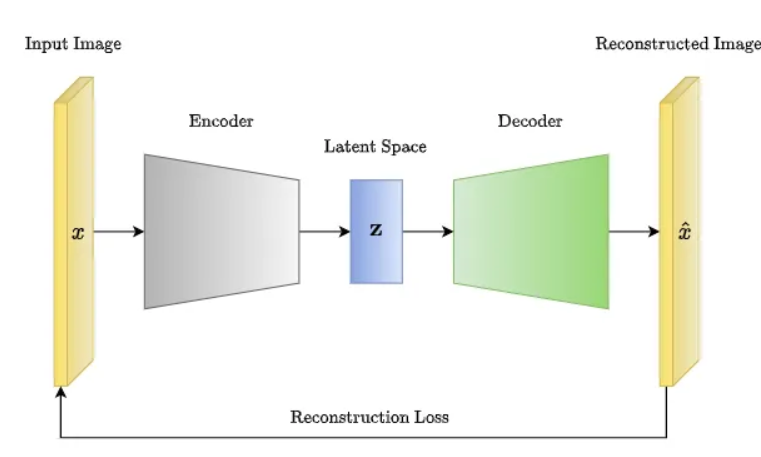
\includegraphics[width=10cm]{images_pfe/vae_1.png}
	\caption{Le fonctionnement d'un neurone artificiel [\cite{kingma_welling_auto_encoding}].}
	\label{fig:VAE}
\end{figure}

\subsection{Applications des Auto-Encodeurs Variationnels (VAE)}

Les auto-encodeurs variationnels (VAE) ont démontré leur efficacité dans divers
domaines grâce à leur capacité à apprendre des représentations latentes
significatives. Voici quelques-unes des principales applications des VAE :

\subsubsection{Génération d'Images}

Les VAE sont largement utilisés pour générer des images réalistes. En apprenant
une représentation latente des images d'entraînement, les VAE peuvent
échantillonner de cet espace latent pour créer de nouvelles images qui
partagent des caractéristiques similaires avec les données d'origine. Cela a
des applications potentielles dans la création de contenu, la conception
assistée par ordinateur et la synthèse d'images médicales [\cite{luhman2024highfidelity}].

\subsubsection{Synthèse de Texte}

Les VAE peuvent être appliqués à la génération de texte en apprenant les
structures latentes des séquences de texte. Ils permettent de produire des
phrases cohérentes et des paragraphes qui imitent le style et le contenu des
textes d'entraînement. Cette technique est utile dans des domaines tels que la
génération automatique de rapports, l'écriture créative assistée et la
traduction automatique[\cite{wang2019topic}].

\subsubsection{Compression de Données}

Les VAE sont efficaces pour la compression de données, en particulier pour des
données de grande dimension comme les images et les vidéos. En apprenant une
représentation latente compacte, les VAE peuvent réduire la dimensionnalité des
données tout en préservant leurs caractéristiques essentielles. Cela permet une
transmission et un stockage plus efficaces des données compressées[\cite{yilmaz2021selfvae}].

\subsubsection{Détection d'Anomalies}

Dans les systèmes de détection d'anomalies, les VAE peuvent être utilisés pour
identifier des données aberrantes qui diffèrent significativement des données
d'entraînement. En apprenant une distribution latente des données normales, le
VAE peut détecter des échantillons qui ne correspondent pas à cette
distribution, ce qui est particulièrement utile dans la surveillance de
systèmes industriels, la cybersécurité et la détection de fraudes [\cite{wang2019revisiting}].

\subsubsection{Imputation de Données Manquantes}

Les VAE peuvent également être employés pour l'imputation de données
manquantes. En apprenant la structure latente des données complètes, les VAE
peuvent estimer les valeurs manquantes de manière cohérente avec les données
observées. Cette application est cruciale dans des domaines tels que l'analyse
de données médicales, les études socio-économiques et les bases de données
incomplètes [\cite{collier2020vaes}].

En résumé, les VAE sont des outils polyvalents dans le domaine de
l'apprentissage machine, avec des applications variées allant de la génération
de contenu à la compression de données et à la détection d'anomalies. Leur
capacité à apprendre des représentations latentes significatives permet de
traiter efficacement une large gamme de problèmes complexes.

\section{Réseaux Antagonistes Génératifs (GANs)}

\subsection{Introduction aux Réseaux Antagonistes Génératifs}

Les réseaux antagonistes génératifs, ou Generative Adversarial Networks (GANs)
en anglais, sont une classe de modèles génératifs introduite par Ian Goodfellow
et ses collègues en 2014 [\cite{goodfellow2014generative}]. Les GANs se
composent de deux réseaux de neurones concurrents : un générateur et un
discriminateur. Le générateur cherche à produire des échantillons réalistes à
partir d'un bruit aléatoire, tandis que le discriminateur tente de distinguer
les échantillons réels des échantillons générés. Cette compétition incite les
deux réseaux à s'améliorer simultanément, aboutissant à la génération de
données de haute qualité.

\subsection{Fonctionnement des GANs}

Les GANs sont des modèles très performants et sont adaptés à plusieurs
architectures variées. Cependant, ils se composent principalement de deux
réseaux de neurones principaux :

\subsubsection{Générateur}

Le réseau générateur prend un vecteur de bruit \( z \) tiré d’une distribution
uniforme ou normale et produit une donnée synthétique \( G(z) \).
Mathématiquement, le générateur peut être représenté comme une fonction \( G :
Z \rightarrow X \), où \( Z \) est l'espace du bruit et \( X \) est l'espace
des données. L’objectif du générateur est de "tromper" le discriminateur en
générant des données indiscernables des données réelles.

\begin{equation}
    G(\mathbf{z}; \theta_g) : \mathbf{z} \sim p_z(\mathbf{z}) \rightarrow \mathbf{x} = G(\mathbf{z})
\end{equation}


où \( \theta_g \) représente les paramètres du générateur, \( p_z(z) \) est la
distribution du bruit (généralement uniforme ou normale), et \( x \) est la
donnée synthétique générée.

Le générateur apprend à partir des erreurs du discriminateur, en améliorant
constamment la qualité des données générées. En d'autres termes, il essaie de
maximiser la probabilité que le discriminateur classifie ses sorties comme
étant des données réelles.

\subsubsection{Discriminateur}

Le réseau discriminateur reçoit soit une donnée réelle \( x \) soit une donnée
générée \( G(z) \). Il sort une probabilité \( D(x) \) ou \( D(G(z)) \)
indiquant si l’entrée est réelle ou générée. Mathématiquement, le
discriminateur peut être représenté comme une fonction \( D : X \rightarrow [0,
	1] \), où \( D(x) \) représente la probabilité que \( x \) soit une donnée
réelle.

\begin{equation}
    D(\mathbf{x}; \theta_d) : \mathbf{x} \rightarrow [0, 1]
\end{equation}


où \( \theta_d \) représente les paramètres du discriminateur. Le
discriminateur est entraîné pour maximiser la probabilité d’assigner la bonne
étiquette aux échantillons réels et générés. Il essaie de minimiser la
probabilité d'être trompé par les fausses données produites par le générateur.

Le discriminateur est, en essence, un classificateur binaire qui essaie de
distinguer entre les données authentiques et celles générées.

\subsubsection{Fonction de Perte}

Les fonctions de perte pour le générateur et le discriminateur sont définies
comme suit :

\begin{equation}
    \mathcal{L}_D = -\mathbb{E}_{\mathbf{x} \sim p_{data}}[\log D(\mathbf{x})] - \mathbb{E}_{\mathbf{z} \sim p_z}[\log(1 - D(G(\mathbf{z})))]
\end{equation}

\begin{equation}
    \mathcal{L}_G = -\mathbb{E}_{\mathbf{z} \sim p_z}[\log D(G(\mathbf{z}))]
\end{equation}

Où :
\begin{conditions}
	\mathcal{L}_D & fonction de perte du discriminateur \\
	\mathcal{L}_G & fonction de perte du générateur \\
	x & donnée réelle tirée de la distribution \( p_{data} \) \\
	z & vecteur de bruit tiré de la distribution \( p_z \) \\
	D(x) & probabilité estimée par le discriminateur que \( x \) soit une donnée réelle \\
	G(z) & donnée synthétique générée à partir du bruit \( z \)
\end{conditions}

L'objectif du générateur est de minimiser \( \mathcal{L}_G \), tandis que le
discriminateur cherche à minimiser \( \mathcal{L}_D \). Plus formellement,
l'objectif est de résoudre le problème de minimax suivant :

\begin{equation}
    \min_G \max_D \mathbb{E}_{\mathbf{x} \sim p_{data}}[\log D(\mathbf{x})] + \mathbb{E}_{\mathbf{z} \sim p_z}[\log(1 - D(G(\mathbf{z})))]
\end{equation}

\subsubsection{Entraînement des GANs}

L’entraînement des réseaux antagonistes génératifs (GANs) implique une série
d'étapes répétitives où le générateur et le discriminateur sont mis à jour tour
à tour pour améliorer leurs performances respectives. Le processus se déroule
comme suit :

L'entraînement des GANs se fait par les étapes suivantes :
\begin{enumerate}
	\item Tirer un échantillon de bruit \( z \) de la distribution \( p_z \).
	\item Générer une donnée synthétique \( G(z) \) à partir du générateur.
	\item Tirer un échantillon de données réelles \( x \) de la distribution de données
	      \( p_{data} \).
	\item Mettre à jour les poids du discriminateur \( D \) en minimisant la fonction de
	      perte \( \mathcal{L}_D \).
	\item Tirer un nouvel échantillon de bruit \( z \).
	\item Mettre à jour les poids du générateur \( G \) en minimisant la fonction de
	      perte \( \mathcal{L}_G \).
	\item Répéter les étapes ci-dessus pour un nombre prédéfini d'itérations.
\end{enumerate}

En suivant ces étapes, les GANs sont entraînés pour générer des données
synthétiques réalistes qui peuvent être utilisées dans diverses applications,
telles que la génération d'images, la super-résolution d'images et la synthèse
de texte.

\begin{figure}[hbt!]
	\centering
	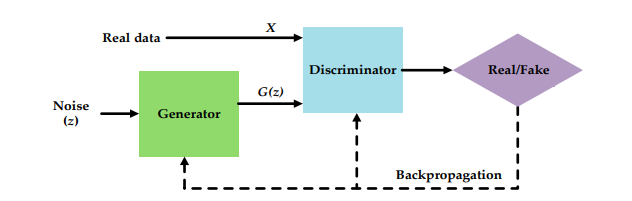
\includegraphics[width=12cm]{images_pfe/gan_1.png}
	\caption{Un modèle de réseau générateur adversaire (GAN) [\cite{feng_feng_chen_cao_zhang_jiao_yu_2020}].}
	\label{fig:gan}
\end{figure}
\FloatBarrier

\subsection{Applications des GANs}

Les GANs ont une variété d'applications dans différents domaines :

\subsubsection{Génération d'Images}

Les GANs sont largement utilisés pour générer des images réalistes. Ils ont été
appliqués avec succès dans la création d'images de haute qualité, la génération
de visages humains, et même la création artistique. Par exemple, les GAN
peuvent générer des images de personnes qui n'existent pas en apprenant les
caractéristiques des visages humains à partir de vastes bases de données
d'images.

\subsubsection{Super-Résolution d'Images}

Les GANs sont également utilisés pour la super-résolution d'images,
c'est-à-dire augmenter la résolution d'une image basse résolution. Le modèle
SRGAN (Super-Resolution GAN) est un exemple où les GANs sont utilisés pour
produire des images de haute résolution à partir d'images de basse résolution,
améliorant ainsi les détails visuels et la clarté.

\subsubsection{Synthèse de Texte et Traduction Automatique}

Dans le traitement du langage naturel (NLP), les GANs sont appliqués à la
génération de texte et à la traduction automatique. Les modèles basés sur les
GAN peuvent générer des phrases cohérentes et contextuellement appropriées,
imitant le style et le contenu des textes d'entraînement. Cela est
particulièrement utile pour les applications comme les chatbots, la création de
contenu textuel, et les systèmes de traduction.

\subsubsection{ StyleGAN: This Person Does Not Exist}

StyleGAN, ou Style-Based Generator Architecture for Generative Adversarial
Networks, est un modèle génératif avancé développé par les chercheurs de
NVIDIA[\cite{karras2019style}]. Il représente une avancée significative dans la
génération d'images de haute qualité et photoréalistes, y compris les visages
de personnes qui n'existent pas. StyleGAN a diverses applications, y compris
dans l'industrie du divertissement, la réalité virtuelle et la recherche
académique.

\textbf{This Person Does Not Exist}: Un exemple frappant de l'application de StyleGAN est le site web "This Person Does Not Exist" [\cite{thispersondoesnotexist}]  . Ce site utilise un modèle StyleGAN pour générer de manière aléatoire des visages de personnes qui n'existent pas à chaque rechargement de la page.

\begin{figure}[hbt!]
	\centering
	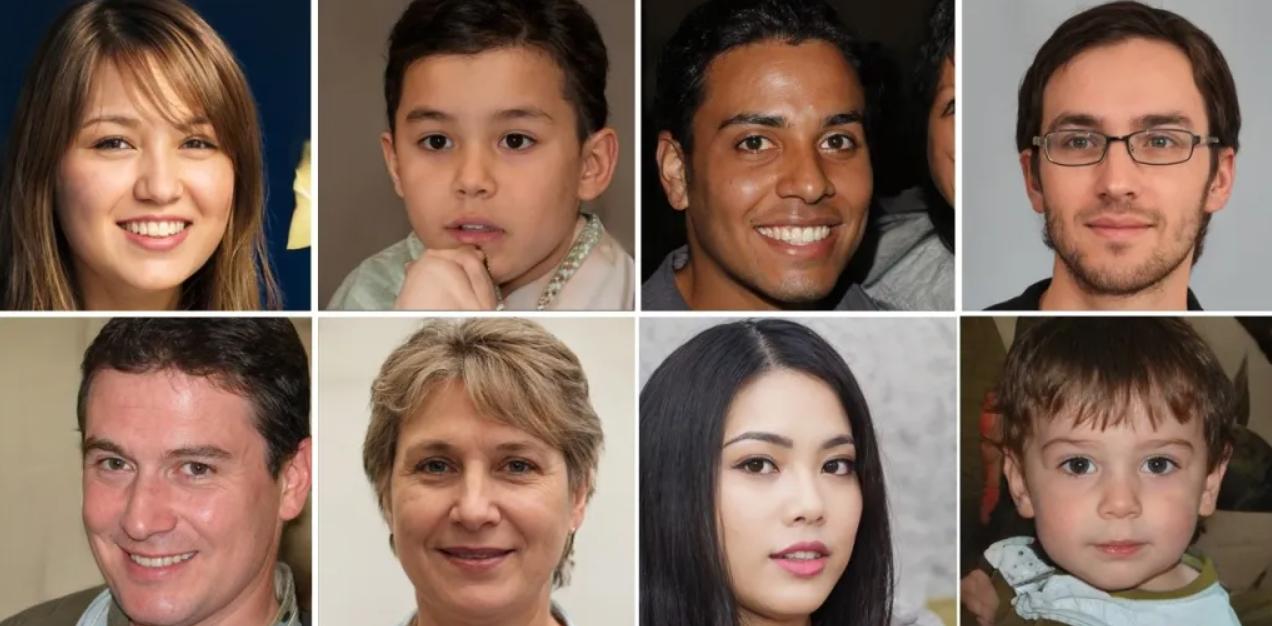
\includegraphics[width=12cm]{images_pfe/thisperson.png}
	\caption{Quelques images générées par le modèle StyleGAN sur le site 'This Person Does Not Exist'[\cite{thispersondoesnotexist}].}
	\label{fig:thisperson}
\end{figure}
\FloatBarrier

En résumé, les GANs sont des outils puissants et polyvalents dans le domaine de
l'apprentissage machine, avec des applications qui vont de la génération
d'images à la traduction automatique. Leur capacité à apprendre et à générer
des données réalistes ouvre de nombreuses perspectives dans divers domaines.

%%%%%%%%%%%%%%%%%%%%%%%%%%%%%%%%%%Diffusion Model%%%%%%%%%%%%%%%%%%%%%%%%%%%%%%%%%%%%
\section{Diffusion models}
\subsection{Introduction}

Les modèles de diffusion, également connus sous le nom de diffusion models,
représentent une avancée significative dans le domaine des modèles génératifs
au sein de l'apprentissage automatique. Émergents de manière proéminente ces
dernières années, ces modèles ont attiré l'attention pour leur remarquable
capacité à générer des données synthétiques de haute qualité, les positionnant
comme une alternative prometteuse aux techniques plus établies telles que les
Réseaux Antagonistes Génératifs (GANs) et les Autoencodeurs Variationnels
(VAEs) [\cite{dhariwal2021diffusion}].

La fondation conceptuelle des modèles de diffusion s'inspire des processus de
diffusion physique, où les particules migrent des régions de haute
concentration vers des zones de moindre concentration [\cite{ho2020denoising}]
. Ces modèles sont également basés sur les chaînes de Markov comme illustré
dans la figure (2.4), un concept clé en probabilité qui décrit une série de
transitions d'état où chaque état dépend uniquement de l'état précédent. Dans
le contexte des données, ce principe est exploité pour affiner progressivement
les données bruitées en représentations réalistes [\cite{yang2022diffusion}].

\begin{figure}[hbt!]
	\centering
	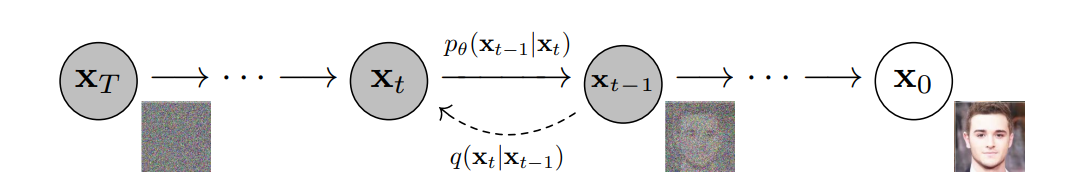
\includegraphics[width=12cm]{images_pfe/markov.png}
	\caption{Chaîne de Markov du processus de diffusion [\cite{ho2020denoising}].}
	\label{fig:markov}
\end{figure}
\FloatBarrier

\subsection{Fonctionnement des Modèles de Diffusion}

Les modèles de diffusion utilisent un processus en deux étapes cruciales : le
bruitage (noising, également appelé Forward Process) et le débruitage
(denoising, ou Reverse Process). Ces étapes sont essentielles pour transformer
des données réelles en une distribution de bruit et inversement. Le Forward
Process consiste à ajouter progressivement du bruit aux données réelles, les
transformant ainsi en une séquence de données de plus en plus bruitées.
Ensuite, le Reverse Process inverse ce processus en éliminant le bruit étape
par étape, recréant des données réalistes à partir du bruit.

Pour effectuer le débruitage, un réseau de neurones est utilisé. Ce réseau de
neurones est entraîné à détecter et à éliminer le bruit à chaque étape du
Reverse Process. Il apprend à prédire l'état précédent des données à partir de
l'état actuel bruité, permettant ainsi de reconstruire progressivement les
données originales. Cette méthode en deux phases, combinée à l'utilisation d'un
réseau de neurones pour le débruitage, permet de modéliser et de générer des
données synthétiques de haute qualité de manière efficace et contrôlée.

\begin{figure}[hbt!]
	\centering
	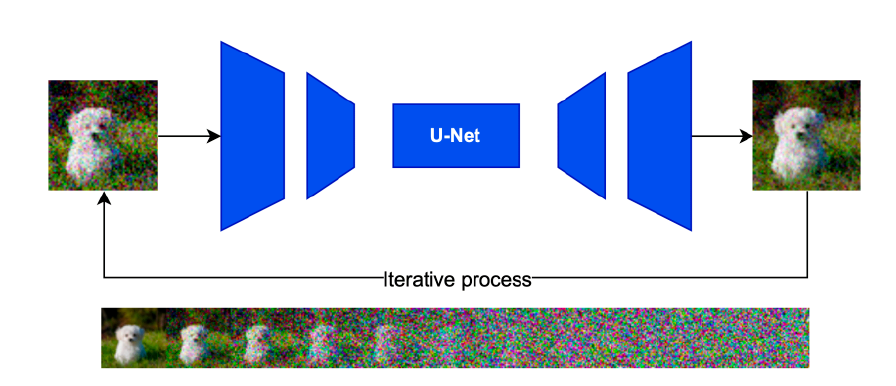
\includegraphics[width=12cm]{images_pfe/Unet.png}
	\caption{ Le processus d'entraînement d'un UNet pour prédire le bruit ajouté à l'image. [\cite{nichol2021improved}].}
	\label{fig:unet}
\end{figure}
\FloatBarrier

Les modèles de diffusion utilisent un processus en deux étapes : le bruitage
(noising, également appelé \textit{Forward Process}) et le débruitage
(denoising, ou \textit{Reverse Process}). Ces étapes sont essentielles pour
transformer des données réelles en une distribution de bruit et inversement.

\subsubsection{Forward Process (Bruitage)}

L'étape de bruitage ajoute progressivement du bruit gaussien aux données
réelles. Ce processus est modélisé comme une chaîne de Markov où chaque état \(
x_t \) dépend uniquement de l'état précédent \( x_{t-1} \).

La transition conditionnelle pour le bruitage est donnée par :
\begin{equation}
    q(\mathbf{x}_t \mid \mathbf{x}_{t-1}) = \mathcal{N}(\mathbf{x}_t; \sqrt{1 - \beta_t} \mathbf{x}_{t-1}, \beta_t \mathbf{I})
\end{equation}


où :
\begin{conditions}
	x_t & \text{état des données à l'étape \( t \)} \\
	\beta_t & \text{taux de bruitage (un hyperparamètre ou une fonction du temps)} \\
	\mathcal{N} & \text{distribution normale gaussienne} \\
	\mathbf{I} & \text{matrice identité}
\end{conditions}

La séquence complète des \( T \) étapes de bruitage est décrite par :
\begin{equation}
    q(\mathbf{x}_{1:T} \mid \mathbf{x}_0) = \prod_{t=1}^T q(\mathbf{x}_t \mid \mathbf{x}_{t-1})
\end{equation}

\textbf{Explication du Forward Process :}

\begin{itemize}
	\item À chaque étape \( t \), une petite quantité de bruit gaussien est ajoutée à \( x_{t-1} \), produisant \( x_t \).
	\item La moyenne de la distribution est \( \sqrt{1 - \beta_t} x_{t-1} \), indiquant
	      que la contribution des données d'origine diminue progressivement.
	\item La variance est \( \beta_t \), contrôlant la quantité de bruit ajouté.
\end{itemize}

\subsubsection{Reverse Process (Débruitage)}

L'étape de débruitage consiste à inverser le processus de bruitage pour
transformer le bruit gaussien en données réalistes. Cela se fait en utilisant
un modèle génératif pour approximer la distribution inverse.

La transition conditionnelle pour le débruitage est donnée par :

\begin{equation}
    p_\theta(\mathbf{x}_{t-1} \mid \mathbf{x}_t) = \mathcal{N}(\mathbf{x}_{t-1}; \mu_\theta(\mathbf{x}_t, t), \Sigma_\theta(\mathbf{x}_t, t))
\end{equation}


où :
\begin{conditions}
	p_\theta & \text{distribution paramétrée par les poids du modèle \( \theta \)} \\
	\mu_\theta & \text{moyenne apprise par le modèle} \\
	\Sigma_\theta & \text{covariance apprise par le modèle}
\end{conditions}

\textbf{Explication du Reverse Process :}

\begin{itemize}
	\item Le modèle est entraîné pour prédire \( x_{t-1} \) à partir de \( x_t \).
	\item La moyenne \( \mu_\theta(x_t, t) \) est une fonction paramétrée par \( \theta
	      \), dépendant de \( x_t \) et du temps \( t \).
	\item La covariance \( \Sigma_\theta(x_t, t) \) représente l'incertitude du modèle.
\end{itemize}

\begin{figure}[hbt!]
	\centering
	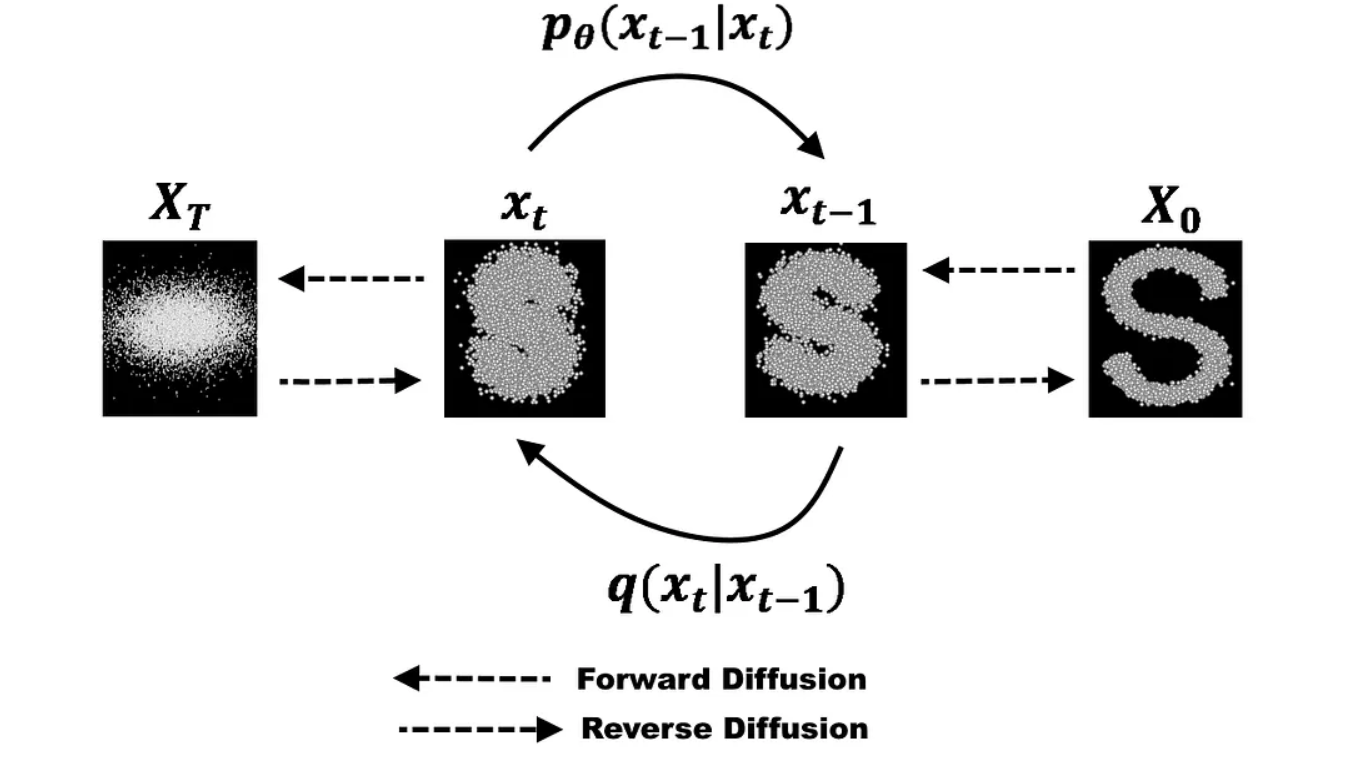
\includegraphics[width=12cm]{images_pfe/diffusion_process.png}
	\caption{Illustration des Processus de Diffusion : Forward Process et Reverse Process.}
	\label{fig:markov}
\end{figure}
\FloatBarrier

\paragraph{Objectif d'Entraînement :}
L'objectif est de minimiser la divergence de Kullback-Leibler (KL) entre la
distribution réelle \( q \) et la distribution générée par le modèle \(
p_\theta \) :

\begin{equation}
    \mathcal{L} = \mathbb{E}_q \left[ \sum_{t=1}^T D_{KL}(q(\mathbf{x}_{t-1} \mid \mathbf{x}_t, \mathbf{x}_0) \| p_\theta(\mathbf{x}_{t-1} \mid \mathbf{x}_t)) \right]
\end{equation}

\subsection{Applications des Modéles de Diffusion}
Les modèles de diffusion ont trouvé des applications dans divers domaines grâce
à leur capacité à générer des données synthétiques de haute qualité. Voici
quelques-unes des applications les plus remarquables :

\begin{itemize}
	\item \textbf{Génération d'images} : Les modèles de diffusion sont largement utilisés pour la génération d'images réalistes à partir de bruit aléatoire. Ils permettent de créer des images de haute qualité qui peuvent être utilisées dans le domaine de l'art, du design, et même dans la production de contenu multimédia.

	\item \textbf{Synthèse vocale} : Ces modèles sont également appliqués dans la génération de voix synthétiques, offrant des améliorations significatives dans la clarté et la naturalité de la voix produite, utilisée dans les assistants vocaux et les technologies de lecture automatique.

	\item \textbf{Création de vidéos} : En transformant des séquences de bruit en vidéos cohérentes, les modèles de diffusion peuvent générer des animations et des vidéos synthétiques, ouvrant de nouvelles possibilités dans le divertissement et la publicité.

	\item \textbf{Traitement et amélioration d'images} : Les modèles de diffusion peuvent être utilisés pour restaurer des images bruitées, améliorer la résolution des images, et effectuer des transformations d'image avancées telles que la colorisation et le changement de style.

	\item \textbf{Séries temporelles} : On peut aussi utiliser les modèles de diffusion pour d'autres types de données comme les séries temporelles. Ils peuvent aider à la prévision, à la détection d'anomalies et à la génération de nouvelles séries temporelles synthétiques [\cite{yang2023survey}].
\end{itemize}

Parmi les applications ayant connu un succès notable, on trouve :

\begin{itemize}
	\item \textbf{Stable Diffusion} : n modèle de diffusion qui a gagné en popularité pour sa capacité à générer des images d’une qualité exceptionnelle et son utilisation dans divers projets artistiques et commerciaux. Stable Diffusion est particulièrement apprécié pour sa flexibilité et sa robustesse, permettant aux artistes et aux créateurs de générer des œuvres d'art numériques impressionnantes avec un niveau de détail et de réalisme sans précédent. En outre, il est utilisé dans des industries telles que le design graphique, la publicité et même la production cinématographique, démontrant sa vaste applicabilité commerciale.

	\item \textbf{DALL-E de OpenAI} : Ce modèle est capable de créer des images à partir de descriptions textuelles, révolutionnant ainsi la manière dont nous concevons et interagissons avec les images générées par l’intelligence artificielle. DALL-E peut interpréter des descriptions textuelles complexes et générer des images correspondantes, ce qui ouvre de nouvelles possibilités en matière de création de contenu visuel. Par exemple, il peut créer des images de concepts ou d'objets inexistants basés uniquement sur des descriptions verbales, ce qui est extrêmement utile pour le prototypage, l'illustration de concepts et l'innovation créative. DALL-E a été salué pour sa capacité à comprendre et à visualiser des idées abstraites, rendant la technologie accessible et utile pour les designers, les artistes et les innovateurs.
\end{itemize}

\begin{figure}[hbt!]
	\centering
	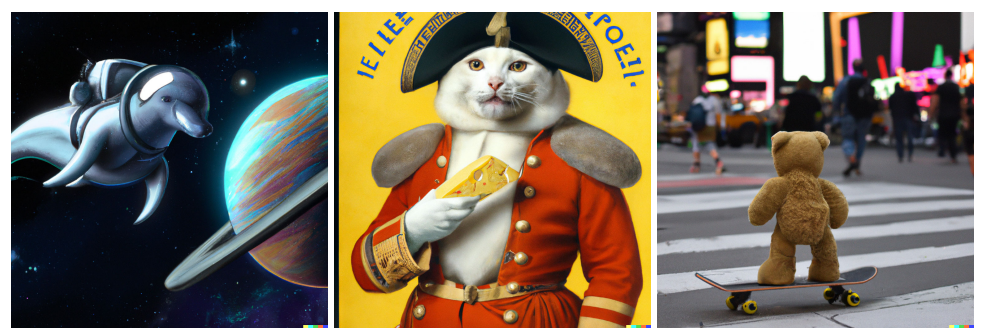
\includegraphics[width=12cm]{images_pfe/sd_images.png}
	\caption{Exemple d’images générée par DALL-E2. [\cite{ramesh2022hierarchical}].}
	\label{fig:unet}
\end{figure}
\FloatBarrier

Ces applications démontrent la polyvalence et l'efficacité des modèles de
diffusion, faisant d'eux des outils indispensables dans l'arsenal de
l'intelligence artificielle moderne.

\subsection{Conclusion}

En conclusion, les modèles de diffusion représentent une avancée significative
dans le domaine des modèles génératifs au sein de l'apprentissage automatique.
En s'appuyant sur un processus en deux étapes, le Forward Process et le Reverse
Process, ces modèles parviennent à transformer des données réelles en une
distribution de bruit et à les reconvertir en données réalistes de haute
qualité. L'utilisation d'un réseau de neurones pour le débruitage améliore
encore l'efficacité et la précision du processus. Grâce à leur capacité à
générer des données synthétiques fiables, les modèles de diffusion se
positionnent comme une alternative prometteuse et robuste aux techniques
traditionnelles telles que les Réseaux Antagonistes Génératifs et les
Autoencodeurs Variationnels. Leur évolution continue et leur adoption
croissante témoignent de leur potentiel immense et de leur pertinence dans
divers domaines d'application de l'intelligence artificielle.

\newpage
%%%%%%%%%%%%%%%%%%%%%%%%%%%%%%%%%% Large Language Models%%%%%%%%%%%%%%%%%%%%%%%%%%%%%%%%%%%%ù

\section{Large Language Models}
Les grands modèles de langage, également connus sous le nom de Large Language
Models (LLM) en anglais, ont révolutionné le domaine de l'intelligence
artificielle en réalisant des avancées significatives dans la génération et la
compréhension du langage naturel. Leur capacité à analyser, traiter et produire
du texte de manière contextuelle et cohérente a ouvert de nouvelles
perspectives dans divers secteurs, notamment la traduction automatique, la
création de contenu et l'assistance virtuelle [\cite{naveed2023overview}].
Parmi les méthodes et techniques employées dans ces modèles de langage, les
réseaux neuronaux de type transformeur occupent une place prépondérante. Ce
type de réseau neuronal sera présenté en détail dans les pages suivantes.

\subsection{Réseaux de Neurones de Transformation (Transformers)}

Les réseaux de neurones de transformation, ou Transformers, sont une
architecture de réseau de neurones introduite par Google. Ils sont
principalement utilisés pour le traitement du langage naturel (NLP), la
traduction de texte et la génération de texte. Les Transformers se distinguent
des réseaux récurrents (RNN) par leur capacité à traiter les dépendances
séquentielles sans utiliser de couches récurrentes. Au lieu de cela, ils
exploitent une technique appelée \textit{self-attention}, permettant au modèle
de se concentrer sur les parties importantes de l'entrée
[\cite{attention_is_all_you_need}].

\subsection{Fonctionnement des Transformers}

\subsubsection{Self-Attention}

Dans un réseau de neurones à auto-attention, chaque mot ou token en entrée est
représenté par un vecteur. Ces vecteurs sont utilisés pour calculer les scores
d’attention entre les différentes parties de l’entrée. La formule de
l’attention pour une tête est donnée par :

\begin{equation}
	\text{Attention}(Q, K, V) = \text{softmax}\left(\frac{QK^T}{\sqrt{d_k}}\right)V
\end{equation}

où $Q$ (queries), $K$ (keys), et $V$ (values) sont des matrices dérivées des
représentations d'entrée, et $d_k$ est la dimension des clés. Ces scores
d'attention pondèrent les vecteurs en entrée, mettant plus d’importance sur les
parties les plus pertinentes [\cite{attention_is_all_you_need}].

\subsubsection{Architecture des Transformers}

L'architecture des Transformers est composée de deux blocs principaux :
l'encodeur et le décodeur.

\paragraph{Bloc d'Encodage}

Un bloc d'encodage transforme une séquence d'entrée $\mathbf{x} = (x_1, x_2,
	\ldots, x_n)$ en une séquence de représentations contextuelles $\mathbf{h} =
	(h_1, h_2, \ldots, h_n)$. Chaque couche d'encodage comprend deux sous-couches
principales :

\begin{itemize}
	\item \textbf{Mécanisme d'Attention Multi-Têtes} : L'attention multi-têtes permet au modèle de se concentrer sur différentes parties de la séquence d'entrée pour chaque mot de sortie.
	\item \textbf{Feed-Forward Network} : Une couche de réseau de neurones feed-forward est appliquée à chaque position de manière indépendante :
	      \begin{equation}
		      \text{FFN}(x) = \max(0, xW_1 + b_1)W_2 + b_2
	      \end{equation}
	      où $W_1$, $W_2$, $b_1$, et $b_2$ sont des paramètres appris.
\end{itemize}

\paragraph{Bloc de Décodage}

Un bloc de décodage génère la séquence de sortie $\mathbf{y} = (y_1, y_2,
	\ldots, y_m)$, en utilisant les représentations contextuelles de l'encodage et
les sorties précédentes. Le bloc de décodage inclut également des sous-couches
d'attention multi-têtes, ainsi que des mécanismes pour l'attention croisée
entre les représentations de l'entrée et de la sortie.

\begin{figure}[hbt!]
	\centering
	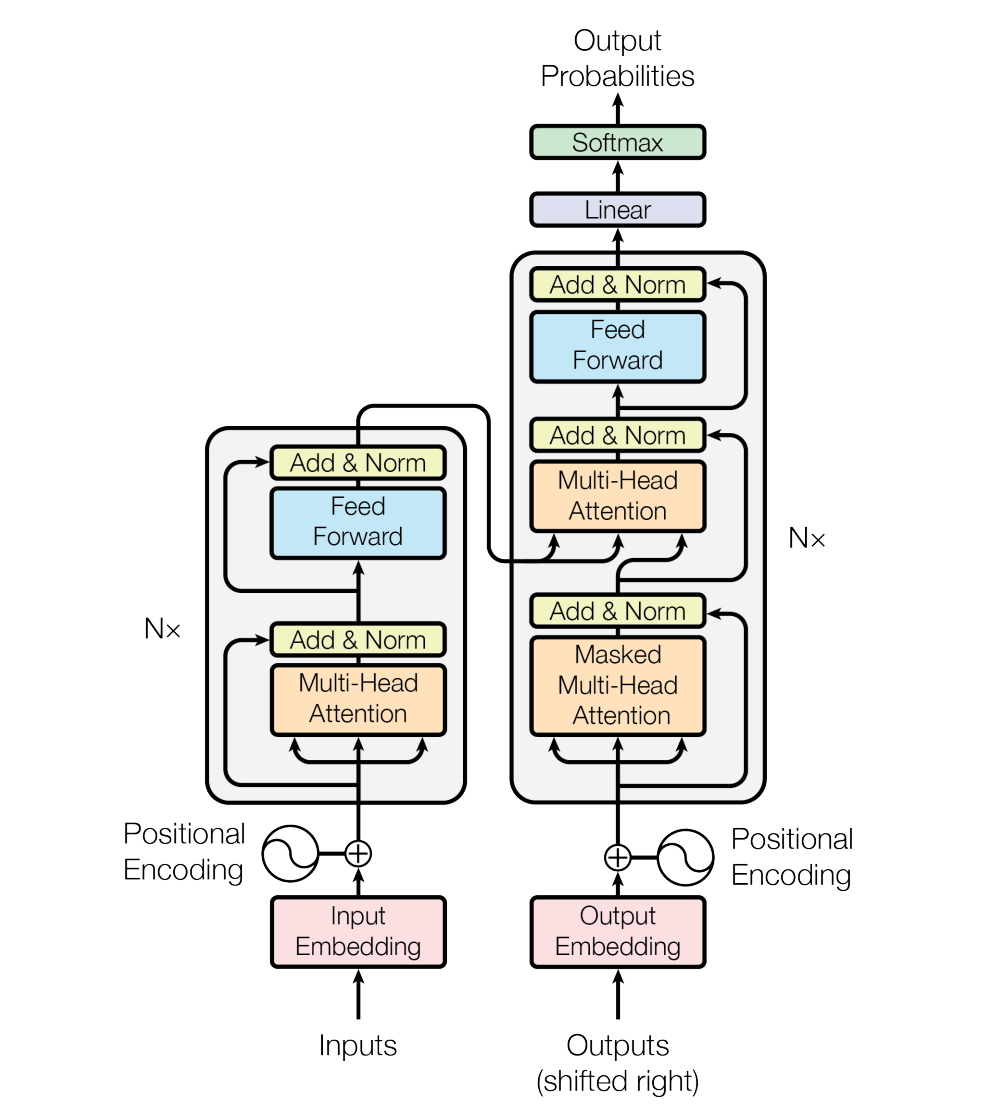
\includegraphics[width=12cm]{images_pfe/transformer-architecture.png}
	\caption{Architecture d'un reseau de neurones de transformation (Transformer) [\cite{attention_is_all_you_need}].}
	\label{fig:transformer}
\end{figure}
\FloatBarrier

\subsection{Applications des Transformers}

\subsubsection{Traduction Automatique}

Les Transformers ont contribué de manière significative aux avancées récentes
dans la traduction automatique. Leur capacité à gérer les dépendances à longue
portée et à traiter les séquences en parallèle leur permet de surpasser les
modèles récurrents traditionnels.

\subsubsection{Génération de Texte}

Les modèles GPT (Generative Pre-trained Transformer) de OpenAI, comme GPT-3,
utilisent des architectures de Transformers massives avec des milliards de
paramètres. Ces modèles sont capables de générer du texte de manière cohérente
et contextuellement pertinente. Par exemple, GPT-3, avec ses 175 milliards de
paramètres, peut produire des textes qui imitent le style et le contenu des
textes d'entraînement [\cite{brown2020language}].

\subsection{Conclusion}

Les Transformers ont révolutionné le domaine du traitement du langage naturel
grâce à leur architecture innovante basée sur le mécanisme de
\textit{self-attention}. Leur capacité à gérer les dépendances séquentielles
sans recourir à des couches récurrentes en fait des outils puissants pour des
applications variées telles que la traduction automatique et la génération de
texte. Les modèles avancés comme GPT-3 de OpenAI démontrent le potentiel énorme
des Transformers lorsqu’ils sont mis à l’échelle avec des milliards de
paramètres.

\chapter{Maintenance prédictive des moteurs électriques}
\section{Introduction}

La maintenance prédictive est devenue une approche incontournable pour la
gestion efficace des équipements industriels, en particulier les moteurs
électriques. Avec l'avènement de l'Industrie 4.0 et l'intégration croissante de
l'Internet des Objets (IoT) et de l'intelligence artificielle (IA) dans les
processus industriels, la maintenance prédictive permet d'anticiper les
défaillances potentielles avant qu'elles ne se produisent, assurant ainsi une
continuité opérationnelle optimale et une réduction significative des coûts de
maintenance [\cite{Mrozek2023}].

Les moteurs électriques, étant au cœur de nombreuses applications
industrielles, représentent des composants critiques dont la fiabilité et
l'efficacité doivent être constamment surveillées. La maintenance prédictive
pour ces moteurs repose sur l'analyse en temps réel de diverses données
opérationnelles telles que les vibrations, les températures, les courants
électriques et les niveaux de bruit. Grâce à des capteurs avancés et à des
algorithmes sophistiqués, il est possible de détecter des anomalies subtiles et
d'identifier les signes précurseurs de défaillances mécaniques ou électriques
[\cite{Bentivogli2023}].

L'adoption de la maintenance prédictive apporte plusieurs avantages majeurs.
Elle permet non seulement d'améliorer la durée de vie des moteurs électriques,
mais aussi de planifier les interventions de maintenance de manière plus
stratégique, évitant ainsi les arrêts imprévus et minimisant les perturbations
de la production. De plus, cette approche contribue à une gestion plus durable
des ressources en réduisant les déchets et en optimisant l'utilisation de
l'énergie.

Dans ce chapitre, nous explorerons en détail les principes fondamentaux de la
maintenance prédictive appliquée aux moteurs électriques. Nous examinerons les
technologies et outils utilisés pour la collecte et l'analyse des données,
ainsi que les différentes méthodes d'interprétation des signaux pour prévoir
les défaillances. Enfin, nous discuterons des défis et des perspectives
d'avenir de cette approche, mettant en lumière son rôle crucial dans la
transformation numérique de l'industrie.

\section{Types de Maintenance}

\subsection{Maintenance Corrective}
La maintenance corrective est réalisée après la détection d’une panne ou d’une
défaillance. Son objectif est de remettre l’équipement en état de fonctionner
en corrigeant le défaut[\cite{Sezdi2019}].

La maintenance corrective intervient généralement après l'échec de
l'équipement, lorsque celui-ci cesse de fonctionner comme prévu. Elle est
souvent utilisée dans les industries où le coût de l'arrêt non planifié est
moins critique ou où les équipements ne peuvent pas être surveillés en continu.
Par exemple, dans certaines installations de production manufacturière, les
interventions correctives peuvent être tolérées si les pièces de rechange sont
facilement disponibles et si les réparations peuvent être effectuées
rapidement. Cette méthode est également courante dans les petites entreprises
où les ressources pour une maintenance plus proactive peuvent être limitées.

\subsection{Maintenance Préventive}
La maintenance préventive est effectuée régulièrement selon un calendrier
prédéfini ou en fonction du temps ou du nombre de cycles d’utilisation,
indépendamment de l’état de l’équipement. Elle vise à réduire la probabilité de
défaillance [\cite{Sezdi2019}].

La maintenance préventive repose sur des inspections et des services réguliers
pour éviter les pannes inattendues. Cette méthode est largement adoptée dans
les industries telles que l'aérospatiale, l'automobile et les centrales
électriques où la fiabilité et la sécurité sont critiques. Par exemple, dans
l'industrie aéronautique, les avions subissent des inspections régulières et
des entretiens programmés pour garantir la sécurité des vols et prévenir les
pannes en vol. De même, dans les centrales électriques, des programmes de
maintenance préventive stricts sont mis en place pour assurer un fonctionnement
continu et sûr des générateurs et des turbines.

\subsection{Maintenance Prédictive}
La maintenance prédictive repose sur la surveillance en temps réel et l’analyse
des données de l’équipement pour anticiper les pannes avant qu’elles ne
surviennent. Elle utilise des techniques telles que la vibration, l’analyse
d’huile, l’imagerie thermique, et les données de performance​
[\cite{Bentivogli2023, Sangeetha2017}].

La maintenance prédictive vise à identifier les signes avant-coureurs de
défaillances potentielles en utilisant des technologies avancées. Les capteurs
IoT, les analyses de données et les algorithmes d'apprentissage automatique
sont employés pour surveiller les conditions des équipements en temps réel.
Cette approche est particulièrement utile dans les industries telles que le
pétrole et le gaz, la production d'énergie et la fabrication de haute
précision. Par exemple, dans les centrales éoliennes, les systèmes de
maintenance prédictive surveillent les vibrations et les températures des
composants critiques pour prévenir les pannes coûteuses et prolonger la durée
de vie des équipements. Dans l'industrie manufacturière, elle permet de
maintenir la qualité des produits et d'optimiser les cycles de production en
réduisant les temps d'arrêt imprévus.

\begin{figure}[hbt!]
	\centering
	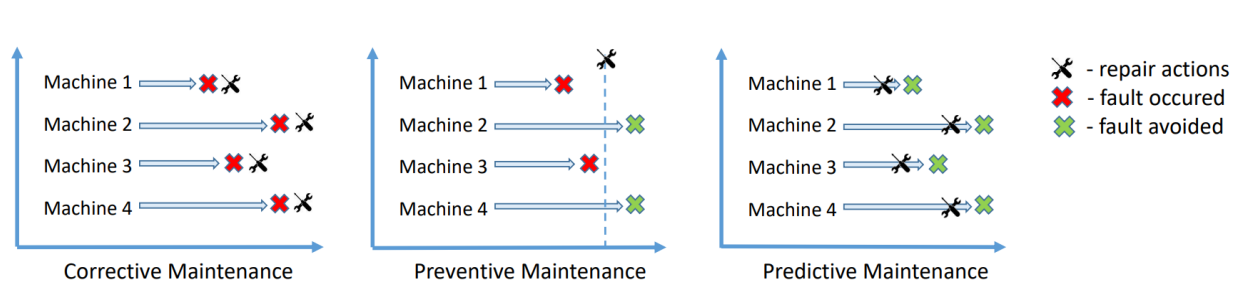
\includegraphics[width=12cm]{images_pfe/predictive.png}
	\caption{Stratégies de maintenance montrant les différentes étapes du processus de réparation avant et après la défaillance potentielle de l'équipement. [\cite{Mrozek2023}].}
	\label{fig:transformer}
\end{figure}
\FloatBarrier

\begin{table}[h]
	\centering
	\begin{tabular}{|l|p{5cm}|p{5cm}|}
		\hline
		\textbf{Type de Maintenance} & \textbf{Avantages}                                                                                                                                            & \textbf{Inconvénients}                                                                                                                   \\
		\hline
		\textbf{Corrective}          & Simple à planifier, nécessite moins de surveillance continue                                                                                                  & Arrêts imprévus, coûts élevés de réparation d’urgence, et perturbations importantes de la production                                     \\
		\hline
		\textbf{Préventive}          & Réduit les risques de pannes imprévues, améliore la fiabilité de l’équipement                                                                                 & Coûts supplémentaires en raison de l’entretien d’équipements encore en bon état, nécessite une planification rigoureuse                  \\
		\hline
		\textbf{Prédictive}          & Permet de planifier les interventions de manière optimale, minimise les arrêts non planifiés, prolonge la durée de vie des équipements, et optimise les coûts & Nécessite des investissements initiaux en capteurs et en technologie de surveillance, ainsi que des compétences analytiques spécialisées \\
		\hline
	\end{tabular}
	\caption{Comparaison entre les Types de Maintenance}
	\label{tab:comparaison-maintenance}
\end{table}

\section{Maintenance prédictive pour les  moteurs électriques }

La maintenance prédictive des moteurs électriques est une approche proactive
qui vise à anticiper les pannes et à optimiser la performance des équipements.
Contrairement à la maintenance réactive, qui intervient après la survenue d'un
problème, ou à la maintenance préventive, qui suit un calendrier fixe, la
maintenance prédictive s'appuie sur la surveillance continue de l'état des
machines et l'analyse de données en temps réel.

Cette stratégie utilise des technologies avancées telles que l'Internet des
objets (IoT), l'intelligence artificielle (IA) et l'analyse de données pour
collecter et interpréter des informations sur les vibrations, la température,
le courant et d'autres paramètres opérationnels des moteurs électriques. Grâce
à ces données, il est possible de détecter les signes avant-coureurs de
défaillances potentielles, comme l'usure des roulements, les déséquilibres de
rotor ou les problèmes d'isolation.

L'objectif principal de la maintenance prédictive est d'améliorer la fiabilité
et la durée de vie des moteurs électriques tout en réduisant les coûts de
maintenance et les interruptions de service. En anticipant les problèmes avant
qu'ils ne deviennent critiques, les entreprises peuvent planifier les
interventions de maintenance de manière plus efficace, minimisant ainsi les
temps d'arrêt imprévus et les coûts associés.

En somme, la maintenance prédictive représente une avancée significative dans
la gestion des actifs industriels, offrant une approche plus intelligente et
efficiente pour la maintenance des moteurs électriques.

\subsection{Moteurs électriques}

Les moteurs électriques sont des dispositifs essentiels qui convertissent
l'énergie électrique en énergie mécanique, jouant un rôle crucial dans de
nombreux aspects de la vie quotidienne et industrielle. Utilisés dans divers
secteurs tels que la fabrication, le transport et les applications domestiques,
les moteurs électriques permettent un contrôle précis, indispensable pour les
applications industrielles nécessitant une régulation rigoureuse de la vitesse
et du couple.

Parmi les différents types de moteurs électriques, les moteurs asynchrones, ou
moteurs à induction, occupent une place prépondérante. Inventés par Nikola
Tesla, ces moteurs sont largement utilisés en raison de leur simplicité, de
leur robustesse et de leur coût relativement bas. Un moteur asynchrone
fonctionne sur le principe de l'induction électromagnétique : lorsqu'un courant
alternatif traverse les bobines du stator, un champ magnétique tournant est
créé, induisant un courant dans le rotor. Ce courant induit génère à son tour
un champ magnétique qui interagit avec celui du stator, produisant un couple
qui fait tourner le rotor.

Ces moteurs sont utilisés dans une vaste gamme d'industries et d'applications.
Dans l'industrie manufacturière, ils entraînent des convoyeurs, des broyeurs et
des compresseurs. Dans les systèmes de traction, ils sont essentiels pour les
trains et les véhicules électriques. De plus, dans les services publics, ils
sont utilisés pour les pompes, les ventilateurs et les systèmes de ventilation
et de climatisation. Les moteurs asynchrones se distinguent par leur fiabilité,
leur capacité à fonctionner dans des conditions difficiles et leur maintenance
relativement facile, ce qui en fait un choix privilégié pour de nombreuses
applications industrielles et domestiques.

\subsubsection{Moteurs Asynchrones}

Il existe deux types de moteurs asynchrones : monophasés et triphasés. Dans
cette section, nous aborderons spécifiquement les moteurs triphas, Dans la
figure (3.2), les principaux composants d'un moteur asynchrone triphasé,
également appelé machine à induction, sont présentés. Voici une description de
chaque composant :

\begin{figure}[hbt!]
	\centering
	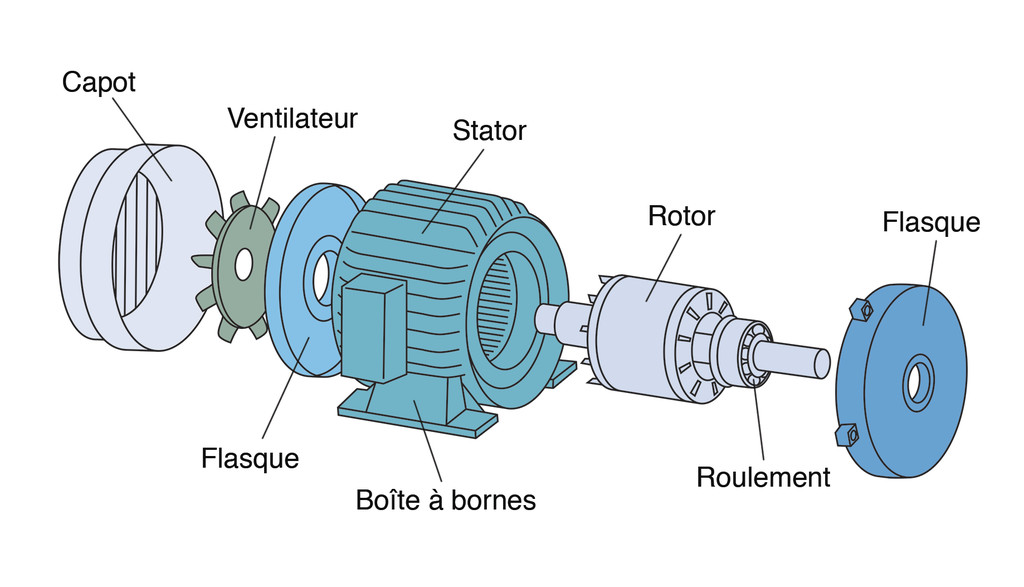
\includegraphics[width=12cm]{images_pfe/motor.jpg}
	\caption{
		Principaux Composants d'un moteur asynchrone triphasé (Machine à Induction).}
	\label{fig:moteu-asynchrone}
\end{figure}
\FloatBarrier

\begin{itemize}
	\item \textbf{Capot} : Il s'agit de la couverture externe du moteur qui protège les composants internes de la poussière, de l'humidité et d'autres contaminants.
	\item \textbf{Ventilateur} : Situé à côté du capot, le ventilateur assure la ventilation du moteur en refroidissant les composants internes pour éviter la surchauffe.
	\item \textbf{Flasque} : Les flasques sont des plaques situées aux extrémités du moteur, qui maintiennent les autres composants en place et assurent l'alignement correct de l'axe du rotor.
	\item \textbf{Stator} : C'est la partie fixe du moteur. Il est constitué de bobines de fil de cuivre qui génèrent un champ magnétique rotatif lorsque le courant triphasé y circule.
	\item \textbf{Boîte à bornes} : Située sur le stator, elle abrite les connexions électriques du moteur, permettant de connecter le moteur à l'alimentation électrique.
	\item \textbf{Rotor} : C'est la partie rotative du moteur qui tourne sous l'effet du champ magnétique généré par le stator. Il est connecté à l'axe et transfère l'énergie mécanique.
	\item \textbf{Roulement} : Les roulements soutiennent le rotor et permettent son mouvement rotatif en minimisant la friction.
\end{itemize}

\subsubsection{Défauts des Moteurs Asynchrones}

Les moteurs asynchrones, également appelés machines à induction, peuvent
présenter divers défauts mécaniques et électriques. Ces défauts peuvent
affecter les performances et la durée de vie du moteur. Voici une description
des principaux défauts mécaniques et électriques :

\paragraph{Défauts Mécaniques}

\subparagraph{Défaut d'excentricité de l'entrefer}:
L'excentricité de l'entrefer se produit lorsque l'espace entre le stator et le
rotor n'est pas uniforme. Cela peut être causé par un désalignement, une usure
inégale des roulements ou des défauts de fabrication. Ce défaut peut entraîner
des vibrations excessives, des bruits anormaux et une usure prématurée des
composants du moteur.

\subparagraph{Analyse des dommages aux roulements}:
Les roulements sont essentiels pour le bon fonctionnement du rotor. Les
dommages aux roulements peuvent être causés par une lubrification insuffisante,
des contaminants, une surcharge ou une mauvaise installation. Les symptômes de
dommages aux roulements incluent des vibrations élevées, des bruits de
grincement ou de cliquetis, et une augmentation de la température de
fonctionnement.

\paragraph{Défauts Électriques}

\subparagraph{Court-circuit entre spires}:
Un court-circuit entre spires se produit lorsque l'isolation entre les
enroulements d'une bobine du stator est endommagée, permettant au courant de
circuler directement entre les spires. Ce défaut peut entraîner une surchauffe
localisée, une diminution de l'efficacité du moteur et, dans les cas graves,
une défaillance complète du moteur.

\subparagraph{Barre de rotor cassée}:
Les barres de rotor sont des composants clés du rotor de la cage d'écureuil
dans un moteur asynchrone. Une barre de rotor cassée peut se produire en raison
de contraintes mécaniques répétées, de surcharges ou de défauts de fabrication.
Ce défaut peut provoquer un déséquilibre du rotor, des vibrations excessives et
une diminution des performances du moteur.

%%%%%%%%%%%%%%%%%%%%%Traitement de Signal%%%%%%%%%%%%%%%%%%%%%ùù

\section{Traitement de Signal Pour les moteurs électriques}

Un signal est une représentation physique ou une mesure de certaines
caractéristiques d’un système, généralement en fonction du temps. Dans le
contexte des moteurs électriques, les signaux peuvent inclure des courants, des
tensions, des vitesses de rotation, des températures, des vibrations, et bien
d'autres paramètres. Ces signaux peuvent être capturés par des capteurs
installés sur ou à proximité du moteur.

L'analyse des signaux de courant et de tension de sortie est cruciale pour la
maintenance prédictive des moteurs électriques. Des techniques telles que
l'analyse des harmoniques, l'analyse du spectre de fréquence et la surveillance
des formes d'onde permettent de détecter les anomalies et de diagnostiquer les
défauts avant qu'ils ne causent des pannes majeures. Par exemple, un
déséquilibre dans les courants de phase peut indiquer un défaut mécanique comme
une excentricité de l'entrefer, tandis qu'une augmentation des harmoniques peut
signaler un court-circuit entre spires.

\subsection*{Signaux Triphasés dans les Moteurs Électriques}

Les moteurs électriques triphasés utilisent des signaux électriques triphasés
pour fonctionner efficacement. Ces signaux, qui consistent en trois courants
alternatifs déphasés de 120 degrés chacun, sont essentiels pour la création
d'un champ magnétique rotatif dans le stator, qui à son tour entraîne la
rotation du rotor.

\subsubsection*{Signaux d'entrée}

Les signaux d'entrée d'un moteur électrique triphasé sont constitués de
courants et de tensions triphasés. Chaque phase est décalée de 120 degrés par
rapport aux autres, permettant une distribution équilibrée de la puissance et
réduisant les vibrations et les pertes. Les courants et tensions triphasés
d'entrée doivent être équilibrés et stables pour assurer un fonctionnement
optimal du moteur. Des déséquilibres ou des variations peuvent indiquer des
problèmes dans l'alimentation ou des défauts internes.

\subsubsection*{Signaux de sortie}

Les signaux de sortie d'un moteur électrique, principalement les courants et
les tensions mesurés aux bornes du moteur, peuvent fournir des informations
précieuses sur l'état de santé du moteur. Un moteur en bon état génère des
signaux de sortie avec un certain motif ou "pattern" caractéristique. Ce motif
est souvent analysé en termes de formes d'onde, d'harmoniques et de spectres de
fréquence.

\begin{figure}[hbt!]
	\centering
	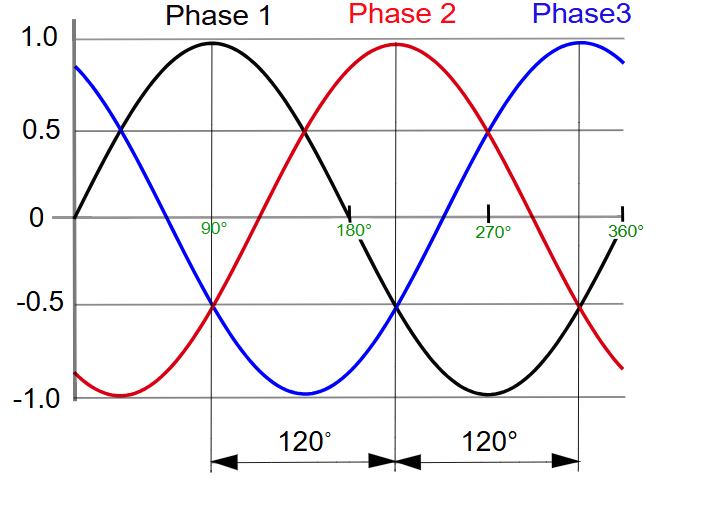
\includegraphics[width=12cm]{images_pfe/triphase.png}
	\caption{
		Principaux Composants d'un moteur asynchrone triphasé (Machine à Induction).}
	\label{fig:moteur-asynchrone}
\end{figure}
\FloatBarrier

\subsection*{Motor Current Signature Analysis (MCSA)}

L'analyse des signaux de courant et de tension de sortie est cruciale pour la
maintenance prédictive des moteurs électriques. Une technique particulièrement
efficace pour cette analyse est la Motor Current Signature Analysis (MCSA).

La MCSA est une méthode de surveillance et de diagnostic basée sur l'analyse
des courants du moteur. En mesurant et en analysant les signatures de courant,
il est possible de détecter des défauts internes et externes du moteur
	[\cite{bonetjara2023sensorless}]. La MCSA peut identifier des problèmes tels
que :
\begin{itemize}
	\item \textbf{Défauts mécaniques} : Excentricité de l'entrefer, désalignement, déséquilibre.
	\item \textbf{Défauts électriques} : Court-circuit entre spires, barres de rotor cassées, défauts d'isolation.
	\item \textbf{Problèmes d'alimentation} : Déséquilibre de phase, distorsions harmoniques.
\end{itemize}

La MCSA utilise des techniques d'analyse de spectre de fréquence pour
identifier les composantes spécifiques du signal de courant qui sont associées
à différents types de défauts. Par exemple, un déséquilibre du rotor peut
générer des fréquences spécifiques qui apparaissent dans le spectre de courant.
En détectant ces fréquences, il est possible de diagnostiquer le défaut avant
qu'il ne cause une panne majeure.

\subsubsection*{Avantages de la MCSA}

L'utilisation de la MCSA pour la surveillance des moteurs électriques présente
plusieurs avantages :
\begin{itemize}
	\item \textbf{Détection précoce des défauts} : Identification des problèmes avant qu'ils ne deviennent critiques.
	\item \textbf{Maintenance proactive} : Planification des interventions de maintenance basées sur l'état réel du moteur.
	\item \textbf{Réduction des coûts} : Minimisation des temps d'arrêt imprévus et des réparations coûteuses.
	\item \textbf{Amélioration de la fiabilité} : Augmentation de la durée de vie des moteurs et amélioration de leur performance globale.
\end{itemize}

la surveillance continue des signaux triphasés et l'utilisation de techniques
comme la MCSA sont essentielles pour assurer le bon fonctionnement et la
longévité des moteurs électriques. L'analyse proactive des courants et des
tensions permet de détecter les problèmes potentiels à un stade précoce,
facilitant ainsi une intervention rapide et réduisant les coûts de maintenance.

\section{Donneés: Séries Temporelles}

Dans de nombreux contextes, les données de séries temporelles peuvent être
considérées comme des signaux, en particulier lorsque les points de données
représentent des mesures prises à intervalles de temps réguliers. Par exemple,
les relevés de température quotidienne constituent une série temporelle qui
peut être analysée comme un signal pour identifier les schémas, les tendances
et les anomalies [\cite{brophy2023gan}] . Il existe deux types de séries
temporelles : discrètes et continues.

Les séries temporelles discrètes, caractérisées par des points de données
espacés à des intervalles réguliers, sont couramment utilisées dans de
nombreuses disciplines pour faciliter l'analyse statistique et la prévision.
Elles permettent une compréhension claire des tendances à long terme et des
variations saisonnières, et sont particulièrement utiles dans des domaines tels
que la climatologie, l'économie et les sciences sociales [\cite{brophy2023gan}]
.

À l'opposé, les séries temporelles continues, où les données sont collectées à des
intervalles infinitésimaux, offrent une représentation plus détaillée et précise des
phénomènes étudiés. Cette approche est cruciale dans des domaines tels que le traitement
du signal, la physique et l'ingénierie, où une résolution temporelle fine est nécessaire
pour capturer les dynamiques rapides et les variations subtiles des systèmes [\cite{brophy2023gan}].

\begin{figure}[hbt!]
	\centering
	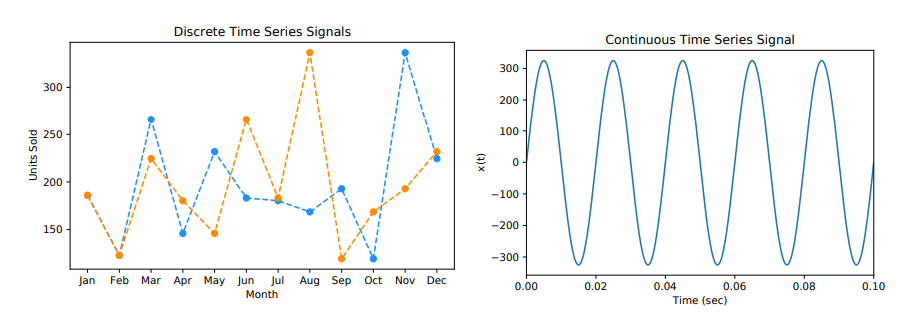
\includegraphics[width=12cm]{images_pfe/timeseries.png}
	\caption{
		Exemples de tracés de séries temporelles discrètes (à gauche) et continues (à droite) [\cite{brophy2023gan}] .}
	\label{fig:time-series}
\end{figure}
\FloatBarrier

\subsubsection{Catégories de Séries Temporelles}

Il existe deux catégories de séries temporelles : univariée et
multivariée[\cite{fawaz2019deep}].

\textbf{Définition 1: Série temporelle univariée}

Une série temporelle univariée $X = [x_1, x_2, \ldots, x_T]$ est un ensemble
ordonné de valeurs réelles. La longueur de $X$ est égale au nombre de valeurs
réelles $T$.

\begin{equation}
	X = [x_1, x_2, \ldots, x_T]
\end{equation}

où $x_i \in \mathbb{R}$ et $i = 1, 2, \ldots, T$.

Par exemple, une série temporelle univariée de température prise toutes les
heures pendant une journée pourrait être représentée par : $X = [15.5, 16.0,
	16.5, \ldots, 20.0]$, où $T = 24$.

\textbf{Définition 2: Série temporelle multivariée}

Une série temporelle multivariée de dimension $M$, notée $X = [X_1, X_2,
	\ldots, X_M]$, se compose de $M$ séries temporelles univariées différentes,
chaque $X_i$ étant un vecteur de $\mathbb{R}^T$.

\begin{equation}
	X = [X_1, X_2, \ldots, X_M]
\end{equation}

où $X_i = [x_{i1}, x_{i2}, \ldots, x_{iT}]$, avec $x_{ij} \in \mathbb{R}$ pour
$i = 1, 2, \ldots, M$ et $j = 1, 2, \ldots, T$.

Par exemple, une série temporelle multivariée de dimension $M=2$, comprenant la
température et l'humidité relevées toutes les heures pendant une journée,
pourrait être représentée par : $X = [X_1, X_2]$, où $X_1$ représente la
température et $X_2$ représente l'humidité, chacun avec $T = 24$.

\section{Conclusion}

La maintenance prédictive des moteurs électriques représente une avancée
significative dans la gestion des actifs industriels, offrant une approche
proactive qui vise à anticiper les pannes et à optimiser la performance des
équipements. Contrairement à la maintenance réactive, qui intervient après la
survenue d’un problème, et à la maintenance préventive, qui suit un calendrier
fixe, la maintenance prédictive repose sur la surveillance continue de l’état
des machines et l’analyse de données en temps réel.

Cette stratégie utilise des technologies avancées telles que l'Internet des
objets (IoT), l'intelligence artificielle (IA) et l'analyse de données pour
collecter et interpréter des informations critiques sur les moteurs
électriques, permettant ainsi de détecter les signes avant-coureurs de
défaillances potentielles. L’objectif principal de cette approche est
d’améliorer la fiabilité et la durée de vie des moteurs électriques tout en
réduisant les coûts de maintenance et les interruptions de service.

En s’appuyant sur des techniques comme la Motor Current Signature Analysis
(MCSA), la maintenance prédictive permet une détection précoce des défauts, une
planification proactive des interventions de maintenance, et une optimisation
des coûts. Cela se traduit par une minimisation des temps d’arrêt imprévus et
une amélioration globale de la performance des moteurs.

Enfin, l'analyse des séries temporelles, qu'elles soient discrètes ou
continues, joue un rôle crucial dans ce processus en fournissant des données
détaillées et précises pour l'analyse des signaux et l'identification des
anomalies. La distinction entre séries temporelles univariées et multivariées
enrichit encore cette approche, permettant une analyse plus complète et
intégrée des différentes variables opérationnelles.

Ainsi, la maintenance prédictive se positionne comme une composante essentielle
de la gestion moderne des moteurs électriques, offrant des avantages
significatifs en termes de fiabilité, de coût et de performance.
%\chapter{Étude de l'existant}
\clearpage
\label{sec:organisme}

\section{Introduction}
Lorem ipsum dolor sit amet, consectetur adipiscing elit. Proin posuere euismod neque, non semper nibh viverra sed. Praesent ut varius magna. Fusce ipsum ante, semper nec interdum at, semper et lacus. Nulla ultrices magna a fringilla finibus. Etiam sollicitudin blandit ante. Vivamus blandit rhoncus tincidunt. Morbi sit amet congue purus. Praesent interdum gravida congue. Donec fermentum dui fermentum maximus rutrum.


\section{Présentation de l’organisme d’accueil}
Djezzy Lorem ipsum dolor sit amet, consectetur adipiscing elit. Proin posuere euismod neque, non semper nibh viverra sed. Praesent ut varius magna. Fusce ipsum ante, semper nec interdum at, semper et lacus. Nulla ultrices magna a fringilla finibus. Etiam sollicitudin blandit ante. Vivamus blandit rhoncus tincidunt. Morbi sit amet congue purus. Praesent interdum gravida congue. Donec fermentum dui fermentum maximus rutrum.

\medskip

Djezzy couvre 95 \% de Lorem ipsum dolor sit amet, consectetur adipiscing elit. Proin posuere euismod neque, non semper nibh viverra sed. Praesent ut varius magna. Fusce ipsum ante, semper nec interdum at, semper et lacus. Nulla ultrices magna a fringilla finibus. Etiam sollicitudin blandit ante. Vivamus blandit rhoncus tincidunt. Morbi sit amet congue purus. Praesent interdum gravida congue. Donec fermentum dui fermentum maximus rutrum., le 1\textsuperscript{er} octobre 2016, dans 20 wilayasLorem ipsum dolor sit amet, consectetur adipiscing elit. Proin posuere euismod neque, non semper nibh viverra sed. Praesent ut varius magna. Fusce ipsum ante, semper nec interdum at, semper et lacus. Nulla ultrices magna a fringilla finibus. Etiam sollicitudin blandit ante. Vivamus blandit rhoncus tincidunt. Morbi sit amet congue purus. Praesent interdum gravida congue. Donec fermentum dui fermentum maximus rutrum..

\medskip

Lorem ipsum dolor sit amet, consectetur adipiscing elit. Proin posuere euismod neque, non semper nibh viverra sed. Praesent ut varius magna. Fusce ipsum ante, semper nec interdum at, semper et lacus. Nulla ultrices magna a fringilla finibus. Etiam sollicitudin blandit ante. Vivamus blandit rhoncus tincidunt. Morbi sit amet congue purus. Praesent interdum gravida congue. Donec fermentum dui fermentum maximus rutrum. L’entreprise est dirigée par \textit{Matthieu Galvani}, Directeur Général.

\medskip

Lorem ipsum dolor sit amet, consectetur adipiscing elit. Proin posuere euismod neque, non semper nibh viverra sed. Praesent ut varius magna. Fusce ipsum ante, semper nec interdum at, semper et lacus. Nulla ultrices magna a fringilla finibus. Etiam sollicitudin blandit ante. Vivamus blandit rhoncus tincidunt. Morbi sit amet congue purus. Praesent interdum gravida congue. Donec fermentum dui fermentum maximus rutrum. \parencite{djezzy_propos_2019}.

Dates clés de Djezzy GSM :
\begin{itemize}
  \item  Octroi de la licence 2G : 30 juillet 2001
  \item  Octroi de la licence 3G : 2 décembre 2013
  \item  Octroi de la licence 4G : 4 septembre 2016
\end{itemize}


\begin{figure}[hbt!]
  \centering
  \includegraphics[width=5cm]{Logo_Djezzy_2015}
  \caption{Logo de Djezzy.}
  \label{fig:logo-djezzy}
\end{figure}
\FloatBarrier

\subsection{VEON}
Lorem ipsum dolor sit amet, consectetur adipiscing elit. Proin posuere euismod neque, non semper nibh viverra sed. Praesent ut varius magna. Fusce ipsum ante, semper nec interdum at, semper et lacus. Nulla ultrices magna a fringilla finibus. Etiam sollicitudin blandit ante. Vivamus blandit rhoncus tincidunt. Morbi sit amet congue purus. Praesent interdum gravida congue. Donec fermentum dui fermentum maximus rutrum.Lorem ipsum dolor sit amet, consectetur adipiscing elit. Proin posuere euismod neque, non semper nibh viverra sed. Praesent ut varius magna. Fusce ipsum ante, semper nec interdum at, semper et lacus. Nulla ultrices magna a fringilla finibus. Etiam sollicitudin blandit ante. Vivamus blandit rhoncus tincidunt. Morbi sit amet congue purus. Praesent interdum gravida congue. Donec fermentum dui fermentum maximus rutrum.\parencite{djezzy_propos_2019}.

\begin{figure}[hbt!]
  \centering
  \includegraphics[width=5cm]{Veon_logo17}
  \caption{Logo de VEON.}
  \label{fig:logo-veon}
\end{figure}
\FloatBarrier

\medskip

\subsection{Vision de Djezzy}
Lorem ipsum dolor sit amet, consectetur adipiscing elit. Proin posuere euismod neque, non semper nibh viverra sed. Praesent ut varius magna. Fusce ipsum ante, semper nec interdum at, semper et lacus. Nulla ultrices magna a fringilla finibus. Etiam sollicitudin blandit ante. Vivamus blandit rhoncus tincidunt. Morbi sit amet congue purus. Praesent interdum gravida congue. Donec fermentum dui fermentum maximus rutrum. \parencite{djezzy_vision_2019}.

\medskip

\subsection{Missions de Djezzy}
Pour réaliser sa vision, Djezzy s'engage à :
\begin{itemize}
  \item  Offrir les meilleurs produits, de qualité, à des prix compétitifs.
  \item  Déployer des infrastructures à la pointe de la technologie.
  \item  Créer pour ses employés le meilleur environnement de travail et d’épanouissement.
  \item Contribuer activement au bien-être des Algériens.
  \item Optimiser la création de valeur pour ses actionnaires, à travers un contrôle strict des coûts.
  \item Appliquer rigoureusement sa politique environnementale.
  \item Améliorer sans cesse ses processus internes dans le respect de sa politique qualité \parencite{djezzy_vision_2019}.
\end{itemize}

\medskip

\subsection{Transformation digitale}
Lorem ipsum dolor sit amet, consectetur adipiscing elit. Proin posuere euismod neque, non semper nibh viverra sed. Praesent ut varius magna. Fusce ipsum ante, semper nec interdum at, semper et lacus. Nulla ultrices magna a fringilla finibus. Etiam sollicitudin blandit ante. Vivamus blandit rhoncus tincidunt. Morbi sit amet congue purus. Praesent interdum gravida congue. Donec fermentum dui fermentum maximus rutrum. \parencite{dabi-schwebel_transformation_2019}. Lorem ipsum dolor sit amet, consectetur adipiscing elit. Proin posuere euismod neque, non semper nibh viverra sed. Praesent ut varius magna. Fusce ipsum ante, semper nec interdum at, semper et lacus. Nulla ultrices magna a fringilla finibus. Etiam sollicitudin blandit ante. Vivamus blandit rhoncus tincidunt. Morbi sit amet congue purus. Praesent interdum gravida congue. Donec fermentum dui fermentum maximus rutrum. :
\begin{itemize}
    \item Rationaliser les ressources (humaines et matérielles ) en centralisant les systèmes d'informations et informatiques.
    \item Réduire les coûts en sous-traitant certains services techniques.
    \item Se positionner dans le monde du digital en proposant de nouveaux services.
    \item Exploiter les opportunités offertes par les nouvelles technologies telles que le Big Data.
    \item Mettre ses employés dans les meilleures conditions de travail pour améliorer la productivité.
\end{itemize}

\medskip


\subsection{Département d'accueil: Service Big Data}
Lorem ipsum dolor sit amet, consectetur adipiscing elit. Proin posuere euismod neque, non semper nibh viverra sed. Praesent ut varius magna. Fusce ipsum ante, semper nec interdum at, semper et lacus. Nulla ultrices magna a fringilla finibus. Etiam sollicitudin blandit ante. Vivamus blandit rhoncus tincidunt. Morbi sit amet congue purus. Praesent interdum gravida congue. Donec fermentum dui fermentum maximus rutrum. :
\begin{itemize}
    \item Permettre à l'entreprise de réagir en temps réel face aux différents changements.
    \item Aider l'entreprise à mieux cibler les clients en répondant à des cas d'utilisation très spécifiques.
    \item Réduire les coûts en exploitant les avantages des technologies Big Data.
    \item Aider les responsables à prendre les décisions adéquates en fournissant les données et les analyses nécessaires.
\end{itemize}

\section{Étude de l'existant}
\label{sec:existant}
Lorem ipsum dolor sit amet, consectetur adipiscing elit. Proin posuere euismod neque, non semper nibh viverra sed. Praesent ut varius magna. Fusce ipsum ante, semper nec interdum at, semper et lacus. Nulla ultrices magna a fringilla finibus. Etiam sollicitudin blandit ante. Vivamus blandit rhoncus tincidunt. Morbi sit amet congue purus. Praesent interdum gravida congue. Donec fermentum dui fermentum maximus rutrum.

\subsection{Recueil d'informations}
Lorem ipsum dolor sit amet, consectetur adipiscing elit. Proin posuere euismod neque, non semper nibh viverra sed. Praesent ut varius magna. Fusce ipsum ante, semper nec interdum at, semper et lacus. Nulla ultrices magna a fringilla finibus. Etiam sollicitudin blandit ante. Vivamus blandit rhoncus tincidunt. Morbi sit amet congue purus. Praesent interdum gravida congue. Donec fermentum dui fermentum maximus rutrum.

\medskip


\begin{xltabular}{\linewidth}{|c|c|c|c|X|}
    \hline
    Num & Date & Type & Service & Points abordés     \\\hline
    1 &  04/11/2019 & Sortie sur terrain & Commercial & Travail de l'animateur  \\[5ex]\hline
    2 &  07/11/2019 & Réunion & Commercial & Explication de la méthode de travail des animateurs  \\\hline
    3 &  07/11/2019 & Réunion & Big Data & Présentation de l’installation technologique de l’entreprise  \\\hline
    4 &  13/11/2019 & Réunion & Commercial & Discussion sur les points de vente  \\\hline
    5 &  25/11/2019 & Réunion & Big Data & Discussion sur l’architecture Big Data de Djezzy  \\\hline
    6 &  27/11/2019 & Réunion & Big Data & Explication de l’architecture globale de Djezzy  \\\hline
    7 &  04/12/2019 & Réunion & Data science & Discussion sur les KPIs pertinents relatifs aux points de vente  \\\hline
    8 &  08/12/2019 & Réunion & Commercial & Discussion sur l’organisation des régions.  \\\hline
    9 &  09/12/2019 & Réunion & Reporting & Discussion sur le reporting des points de vente  \\\hline
    
   
    \caption{L'ensemble des réunions et sorties réalisées.}
    \label{tab:meetings}
\end{xltabular}
\FloatBarrier


\subsection{Réseau de distribution de Djezzy}

Lorem ipsum dolor sit amet, consectetur adipiscing elit. Proin posuere euismod neque, non semper nibh viverra sed. Praesent ut varius magna. Fusce ipsum ante, semper nec interdum at, semper et lacus. Nulla ultrices magna a fringilla finibus. Etiam sollicitudin blandit ante. Vivamus blandit rhoncus tincidunt. Morbi sit amet congue purus. Praesent interdum gravida congue. Donec fermentum dui fermentum maximus rutrum.

\medskip

\begin{figure}[hbt!]
  \centering
  \includegraphics[width=14cm]{images_pfe/reseau_distribution.png}
  \caption{Réseau de distribution de Djezzy.}
  \label{fig:reseau-distribution}
\end{figure}
\FloatBarrier

Lorem ipsum dolor sit amet, consectetur adipiscing elit. Proin posuere euismod neque, non semper nibh viverra sed. Praesent ut varius magna. Fusce ipsum ante, semper nec interdum at, semper et lacus. Nulla ultrices magna a fringilla finibus. Etiam sollicitudin blandit ante. Vivamus blandit rhoncus tincidunt. Morbi sit amet congue purus. Praesent interdum gravida congue. Donec fermentum dui fermentum maximus rutrum.

\medskip

\subsection{Point de vente}
\label{sec:pos}

Lorem ipsum dolor sit amet, consectetur adipiscing elit. Proin posuere euismod neque, non semper nibh viverra sed. Praesent ut varius magna. Fusce ipsum ante, semper nec interdum at, semper et lacus. Nulla ultrices magna a fringilla finibus. Etiam sollicitudin blandit ante. Vivamus blandit rhoncus tincidunt. Morbi sit amet congue purus. Praesent interdum gravida congue. Donec fermentum dui fermentum maximus rutrum.Lorem ipsum dolor sit amet, consectetur adipiscing elit. Proin posuere euismod neque, non semper nibh viverra sed. Praesent ut varius magna. Fusce ipsum ante, semper nec interdum at, semper et lacus. Nulla ultrices magna a fringilla finibus. Etiam sollicitudin blandit ante. Vivamus blandit rhoncus tincidunt. Morbi sit amet congue purus. Praesent interdum gravida congue. Donec fermentum dui fermentum maximus rutrum.

\medskip


\begin{figure}[hbt!]
  \centering
  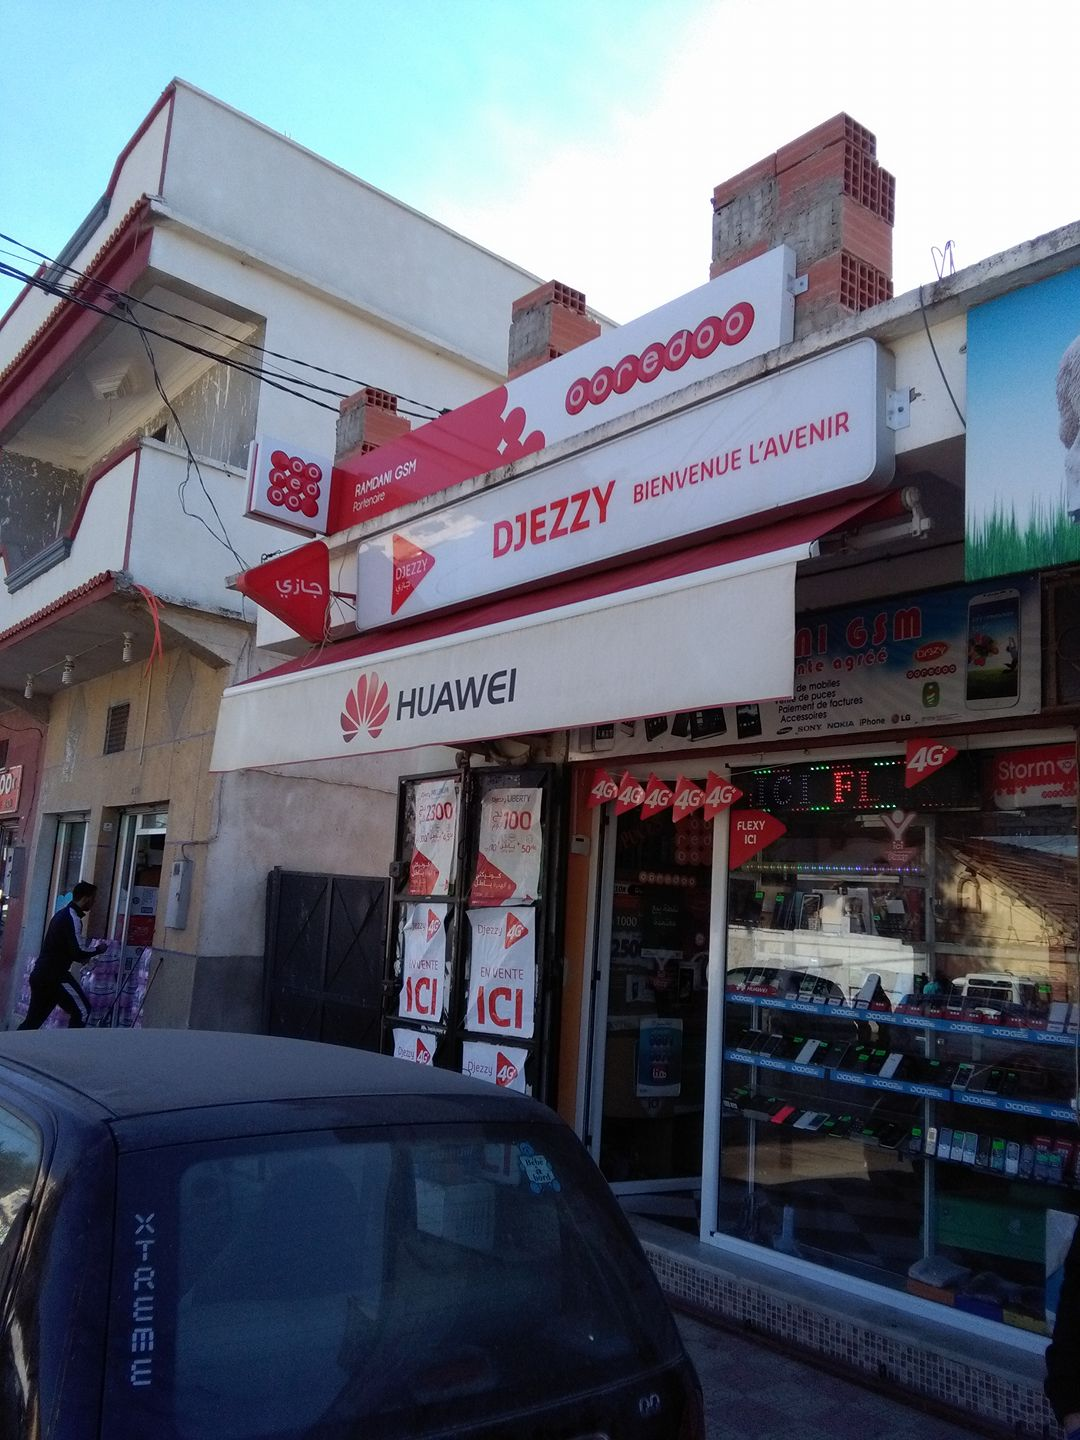
\includegraphics[height=8cm]{images_pfe/point-de-vente.jpg}
  \caption{Un exemple de point de vente Djezzy \parencite{web_image_point_de_vente_2019}.}
  \label{fig:point-de-vente}
\end{figure}
\FloatBarrier

Lorem ipsum dolor sit amet, consectetur adipiscing elit. Proin posuere euismod neque, non semper nibh viverra sed. Praesent ut varius magna. Fusce ipsum ante, semper nec interdum at, semper et lacus. Nulla ultrices magna a fringilla finibus. Etiam sollicitudin blandit ante. Vivamus blandit rhoncus tincidunt. Morbi sit amet congue purus. Praesent interdum gravida congue. Donec fermentum dui fermentum maximus rutrum.Lorem ipsum dolor sit amet, consectetur adipiscing elit. Proin posuere euismod neque, non semper nibh viverra sed. Praesent ut varius magna. Fusce ipsum ante, semper nec interdum at, semper et lacus. Nulla ultrices magna a fringilla finibus. Etiam sollicitudin blandit ante. Vivamus blandit rhoncus tincidunt. Morbi sit amet congue purus. Praesent interdum gravida congue. Donec fermentum dui fermentum maximus rutrum.



\subsection{Animateur de zone}

Lorem ipsum dolor sit amet, consectetur adipiscing elit. Proin posuere euismod neque, non semper nibh viverra sed. Praesent ut varius magna. Fusce ipsum ante, semper nec interdum at, semper et lacus. Nulla ultrices magna a fringilla finibus. Etiam sollicitudin blandit ante. Vivamus blandit rhoncus tincidunt. Morbi sit amet congue purus. Praesent interdum gravida congue. Donec fermentum dui fermentum maximus rutrum.Lorem ipsum dolor sit amet, consectetur adipiscing elit. Proin posuere euismod neque, non semper nibh viverra sed. Praesent ut varius magna. Fusce ipsum ante, semper nec interdum at, semper et lacus. Nulla ultrices magna a fringilla finibus. Etiam sollicitudin blandit ante. Vivamus blandit rhoncus tincidunt. Morbi sit amet congue purus. Praesent interdum gravida congue. Donec fermentum dui fermentum maximus rutrum. :

\medskip

\begin{itemize}
    \item Former et informer les points de vente (produits, offres, challenges, cadeaux...etc.)
    \item Motiver les points de vente pour booster le chiffre d’affaires.
    \item Recueillir et transmettre les informations sur la qualité de réseau, le feedback des clients...etc.
    \item Assurer le marketing (affiches publicitaires, panneau...etc.)
    \item Récupérer les contrats de puces.
    \item Traiter les problèmes des points de vente (activation des puces, Flexy...etc.)
    \item Approbation des nouveaux points de vente.
\end{itemize}

Lorem ipsum dolor sit amet, consectetur adipiscing elit. Proin posuere euismod neque, non semper nibh viverra sed. Praesent ut varius magna. Fusce ipsum ante, semper nec interdum at, semper et lacus. Nulla ultrices magna a fringilla finibus. Etiam sollicitudin blandit ante. Vivamus blandit rhoncus tincidunt. Morbi sit amet congue purus. Praesent interdum gravida congue. Donec fermentum dui fermentum maximus rutrum.Lorem ipsum dolor sit amet, consectetur adipiscing elit. Proin posuere euismod neque, non semper nibh viverra sed. Praesent ut varius magna. Fusce ipsum ante, semper nec interdum at, semper et lacus. Nulla ultrices magna a fringilla finibus. Etiam sollicitudin blandit ante. Vivamus blandit rhoncus tincidunt. Morbi sit amet congue purus. Praesent interdum gravida congue. Donec fermentum dui fermentum maximus rutrum.

\medskip

\begin{figure}[hbt!]
  \centering
  \includegraphics[height=8cm]{images_pfe/animator_route.png}
  \caption{Un exemple de tournée d'un animateur (en rouge).}
  \label{fig:tournee-animateur}
\end{figure}
\FloatBarrier


\medskip

\section{Conclusion}
Lorem ipsum dolor sit amet, consectetur adipiscing elit. Proin posuere euismod neque, non semper nibh viverra sed. Praesent ut varius magna. Fusce ipsum ante, semper nec interdum at, semper et lacus. Nulla ultrices magna a fringilla finibus. Etiam sollicitudin blandit ante. Vivamus blandit rhoncus tincidunt. Morbi sit amet congue purus. Praesent interdum gravida congue. Donec fermentum dui fermentum maximus rutrum.

\medskip

Lorem ipsum dolor sit amet, consectetur adipiscing elit. Proin posuere euismod neque, non semper nibh viverra sed. Praesent ut varius magna. Fusce ipsum ante, semper nec interdum at, semper et lacus. Nulla ultrices magna a fringilla finibus. Etiam sollicitudin blandit ante. Vivamus blandit rhoncus tincidunt. Morbi sit amet congue purus. Praesent interdum gravida congue. Donec fermentum dui fermentum maximus rutrum.






%%% Local Variables: 
%%% mode: latex
%%% TeX-master: "isae-report-template"
%%% End: 
%\chapter{Expression des besoins}
\clearpage
\label{chap:besoins}

\section{Introduction}
Lorem ipsum dolor sit amet, consectetur adipiscing elit. Proin posuere euismod neque, non semper nibh viverra sed. Praesent ut varius magna. Fusce ipsum ante, semper nec interdum at, semper et lacus. Nulla ultrices magna a fringilla finibus. Etiam sollicitudin blandit ante. Vivamus blandit rhoncus tincidunt. Morbi sit amet congue purus. Praesent interdum gravida congue. Donec fermentum dui fermentum maximus rutrum.
\section{Définition des utilisateurs}
Lorem ipsum dolor sit amet, consectetur adipiscing elit. Proin posuere euismod neque, non semper nibh viverra sed. Praesent ut varius magna. Fusce ipsum ante, semper nec interdum at, semper et lacus. Nulla ultrices magna a fringilla finibus. Etiam sollicitudin blandit ante. Vivamus blandit rhoncus tincidunt. Morbi sit amet congue purus. Praesent interdum gravida congue. Donec fermentum dui fermentum maximus rutrum.
\subsection{Administrateur}
Lorem ipsum dolor sit amet, consectetur adipiscing elit. Proin posuere euismod neque, non semper nibh viverra sed. Praesent ut varius magna. Fusce ipsum ante, semper nec interdum at, semper et lacus. Nulla ultrices magna a fringilla finibus. Etiam sollicitudin blandit ante. Vivamus blandit rhoncus tincidunt. Morbi sit amet congue purus. Praesent interdum gravida congue. Donec fermentum dui fermentum maximus rutrum.


\subsection{Animateur}
Lorem ipsum dolor sit amet, consectetur adipiscing elit. Proin posuere euismod neque, non semper nibh viverra sed. Praesent ut varius magna. Fusce ipsum ante, semper nec interdum at, semper et lacus. Nulla ultrices magna a fringilla finibus. Etiam sollicitudin blandit ante. Vivamus blandit rhoncus tincidunt. Morbi sit amet congue purus. Praesent interdum gravida congue. Donec fermentum dui fermentum maximus rutrum.

\clearpage

\section{Spécifications}
Lorem ipsum dolor sit amet, consectetur adipiscing elit. Proin posuere euismod neque, non semper nibh viverra sed. Praesent ut varius magna. Fusce ipsum ante, semper nec interdum at, semper et lacus. Nulla ultrices magna a fringilla finibus. Etiam sollicitudin blandit ante. Vivamus blandit rhoncus tincidunt. Morbi sit amet congue purus. Praesent interdum gravida congue. Donec fermentum dui fermentum maximus rutrum.

\subsection{Spécifications fonctionnelles}
Lorem ipsum dolor sit amet, consectetur adipiscing elit. Proin posuere euismod neque, non semper nibh viverra sed. Praesent ut varius magna. Fusce ipsum ante, semper nec interdum at, semper et lacus. Nulla ultrices magna a fringilla finibus. Etiam sollicitudin blandit ante. Vivamus blandit rhoncus tincidunt. Morbi sit amet congue purus. Praesent interdum gravida congue. Donec fermentum dui fermentum maximus rutrum. :
\renewcommand{\arraystretch}{1.5}
\begin{xltabular}{17cm}{|c|X|}
    \hline
    ID & Description     \\\hline
    1 & Le système doit permettre à l'utilisateur (Administrateur, Animateur) de s'authentifier. \\\hline
    2 & Le système doit permettre à l'administrateur de consulter les statistiques des visites des animateurs. \\\hline
    3 & Le système doit permettre à l'administrateur de consulter la liste des animateurs. \\\hline
    4 & Le système doit permettre à l'administrateur de visualiser les points de vente sur la carte. \\\hline
    5 & Le système doit permettre à l'administrateur de générer les plans de visite des animateurs. \\\hline
    6 & Le système doit permettre à l'administrateur de synchroniser les tournées des animateurs en temps réel (selon les fluctuations du trafic routier). \\\hline
    7 & Le système doit permettre à l'administrateur de visualiser les plans de route des animateurs. \\\hline
    8 & Le système doit permettre à l'administrateur de modifier les paramètres de visite des points de vente. \\\hline
    9 & Le système doit permettre à l'administrateur de choisir les types de points de vente à visiter. \\\hline
    10 & Le système doit permettre à l'animateur de récupérer ses plans de visite. \\\hline
    11 & Le système doit permettre à l'animateur de synchroniser ses tournées en temps réel avec les données du trafic routier. \\\hline
    12 & Le système doit permettre à l'animateur de visualiser ses plans de route sur la carte. \\\hline
    13 & Le système doit classifier les points de vente selon leur degré d'importance. \\\hline
    14 & Le système doit mettre à jour la classification des points de vente selon leur rendement mensuel. \\\hline
    15 & Le système doit inclure l'importance des points de vente dans la logique d'élaboration des plans de visite destinés aux animateurs. \\\hline
    
    \caption{L'ensemble des spécifications fonctionnelles.}
    \label{tab:functional-specs}
\end{xltabular}
\FloatBarrier


\subsection{Spécifications techniques}
Lorem ipsum dolor sit amet, consectetur adipiscing elit. Proin posuere euismod neque, non semper nibh viverra sed. Praesent ut varius magna. Fusce ipsum ante, semper nec interdum at, semper et lacus. Nulla ultrices magna a fringilla finibus. Etiam sollicitudin blandit ante. Vivamus blandit rhoncus tincidunt. Morbi sit amet congue purus. Praesent interdum gravida congue. Donec fermentum dui fermentum maximus rutrum. :

\renewcommand{\arraystretch}{1.5}
\begin{xltabular}{17cm}{|c|X|}
    \hline
    ID & Description     \\\hline
    16 & Le système doit être compatible avec l'architecture de données de Djezzy. \\\hline
    17 & L'architecture du système doit être évolutive. \\\hline
    18 & Le système doit générer les plans de visite en un temps réduit (< 10s). \\\hline
    19 & Le système doit être implémenté sous forme d'une solution web. \\\hline
    20 & Les interfaces du système doivent s'adapter à toutes les tailles d'écrans (responsive). \\\hline
    
    
    \caption{L'ensemble des spécifications techniques.}
    \label{tab:technical-specs}
\end{xltabular}
\FloatBarrier

\section{Définition des cas d'utilisation}

Lorem ipsum dolor sit amet, consectetur adipiscing elit. Proin posuere euismod neque, non semper nibh viverra sed. Praesent ut varius magna. Fusce ipsum ante, semper nec interdum at, semper et lacus. Nulla ultrices magna a fringilla finibus. Etiam sollicitudin blandit ante. Vivamus blandit rhoncus tincidunt. Morbi sit amet congue purus. Praesent interdum gravida congue. Donec fermentum dui fermentum maximus rutrum.Lorem ipsum dolor sit amet, consectetur adipiscing elit. Proin posuere euismod neque, non semper nibh viverra sed. Praesent ut varius magna. Fusce ipsum ante, semper nec interdum at, semper et lacus. Nulla ultrices magna a fringilla finibus. Etiam sollicitudin blandit ante. Vivamus blandit rhoncus tincidunt. Morbi sit amet congue purus. Praesent interdum gravida congue. Donec fermentum dui fermentum maximus rutrum.

\clearpage

\subsection{Administrateur}

\begin{figure}[hbt!]
  \centering
  \includegraphics[ width=\linewidth]{images_pfe/DCU_ADMINISTRATEUR.png}
  \caption{Diagramme des cas d'utilisation de l'administrateur.}
  \label{fig:dcu-administrateur}
\end{figure}
\FloatBarrier


\renewcommand{\arraystretch}{1.5}
\begin{xltabular}{\linewidth}{|c|X|c|c|}
    \hline
    ID & CU & Documentation & Diagramme d'activité     \\\hline
    1 & S'authentifier & & \\ \hline
    2 & Consulter les statistiques des visites & & \\ \hline
    3 & Consulter la liste des animateurs & & \\ \hline
    4 & Visualiser les points de vente sur la carte & & \\ \hline
    5 & Générer les plans de visite des animateurs & \checkmark & \checkmark \\ \hline
    6 & Synchroniser les tournées des animateurs & \checkmark &  \\ \hline
    7 & Visualiser les plans de route des animateurs &  &  \\ \hline 
    8 & Modifier les paramètres de visite des points de vente & \checkmark &  \\ \hline
    9 & Choisir les types de points de vente à visiter & & \\ \hline
    \caption{Liste des cas d'utilisation de l'administrateur.}
    \label{tab:admin-use-cases}
\end{xltabular}
\FloatBarrier


\renewcommand{\arraystretch}{1.5}
\begin{xltabular}{\linewidth}{|X|}
    \hline
    \textbf{CU} : Générer les plans de visite des animateurs     \\\hline
    \textbf{ID} :  5   \\\hline
    \textbf{Description brève} : Générer les plans de visite des animateurs avec les chemins optimaux de parcours  \\\hline
    \textbf{Acteurs primaires} : Administrateur, Temps     \\\hline
    \textbf{Acteurs secondaires} :  /    \\\hline
    \textbf{Pré condition} :  l'administrateur déjà connecté    \\\hline
    \textbf{Enchaînement principal} : \\
    Le cas d'utilisation démarre automatiquement de manière périodique, ou lorsque l'administrateur souhaite générer les plans de visite des animateurs. \\
    1. L'administrateur choisit l'onglet génération des plans. \\
    2. Il introduit la période dans laquelle l'animateur va visiter les points de vente (semaine, 15 jours, mois...etc). \\
    3. Il choisit pour chaque type de point de vente sa fréquence de visite pendant la période. \\
    4. Il lance la génération des plans. \\
    5. Le système génère les plans de visite des animateurs. 
    \\\hline
    \textbf{Post condition} :  Les plans de visite sont générés pour l'ensemble des animateurs   \\\hline
    \textbf{Enchaînement alternatif} :   /   \\\hline
  
    \caption{Documentation CU : Générer les plans de visite des animateurs.}
    \label{tab:cu-specs1}
\end{xltabular}
\FloatBarrier

\clearpage

\renewcommand{\arraystretch}{1.5}
\begin{xltabular}{\linewidth}{|X|}
    \hline
    \textbf{CU} : Synchroniser les tournées des animateurs      \\\hline
    \textbf{ID} :  6    \\\hline
    \textbf{Description brève} : Mettre à jour une tournée d'un animateur par rapport à la fluidité du trafic routier     \\\hline
    \textbf{Acteurs primaires} :  Administrateur    \\\hline
    \textbf{Acteurs secondaires} :  /    \\\hline
    \textbf{Pré condition} :  l'administrateur déjà connecté   \\\hline
    \textbf{Enchaînement principal} : \\
    Le cas d'utilisation démarre lorsque l'administrateur souhaite synchroniser la tournée d'un animateur. \\
    1. L'administrateur choisit la section de synchronisation. \\
    2. Il choisit l'animateur en question. \\
    3. Il lance la synchronisation. \\
    4. Le système synchronise la tournée de l'animateur avec les données du trafic.
    \\\hline
    \textbf{Post condition} : La tournée de l'animateur est mise à jour     \\\hline
    \textbf{Enchaînement alternatif} :   /   \\\hline
    
    \caption{Documentation CU : Synchroniser les tournées des animateurs.}
    \label{tab:cu-specs2}
\end{xltabular}
\FloatBarrier


\renewcommand{\arraystretch}{1.5}
\begin{xltabular}{\linewidth}{|X|}
    \hline
    \textbf{CU} : Modifier les paramètres des visites    \\\hline
    \textbf{ID} :  8   \\\hline
    \textbf{Description brève} : Modifier les paramètres des visites des points de vente      \\\hline
    \textbf{Acteurs primaires} :  Administrateur    \\\hline
    \textbf{Acteurs secondaires} :  /    \\\hline
    \textbf{Pré condition} : L'administrateur est connecté     \\\hline
    \textbf{Enchaînement principal} : \\
    Le cas d'utilisation démarre lorsque l'administrateur souhaite de modifier les paramètres de visite dans le système. \\
    1. L'administrateur introduit la période des visites. \\
    2. L'administrateur introduit les fréquences de visite pour chaque type de point de vente. \\
    3. L'administrateur valide les paramètres.\\
    4. Le système enregistre les nouveaux paramètres.
    \\\hline
    \textbf{Post condition} : Les paramètres des visites sont modifiés     \\\hline
    \textbf{Enchaînement alternatif} :   /   \\\hline
    
    \caption{Documentation CU : Modifier les paramètres de visite.}
    \label{tab:cu-specs3}
\end{xltabular}
\FloatBarrier

\begin{figure}[hbt!]
  \centering
  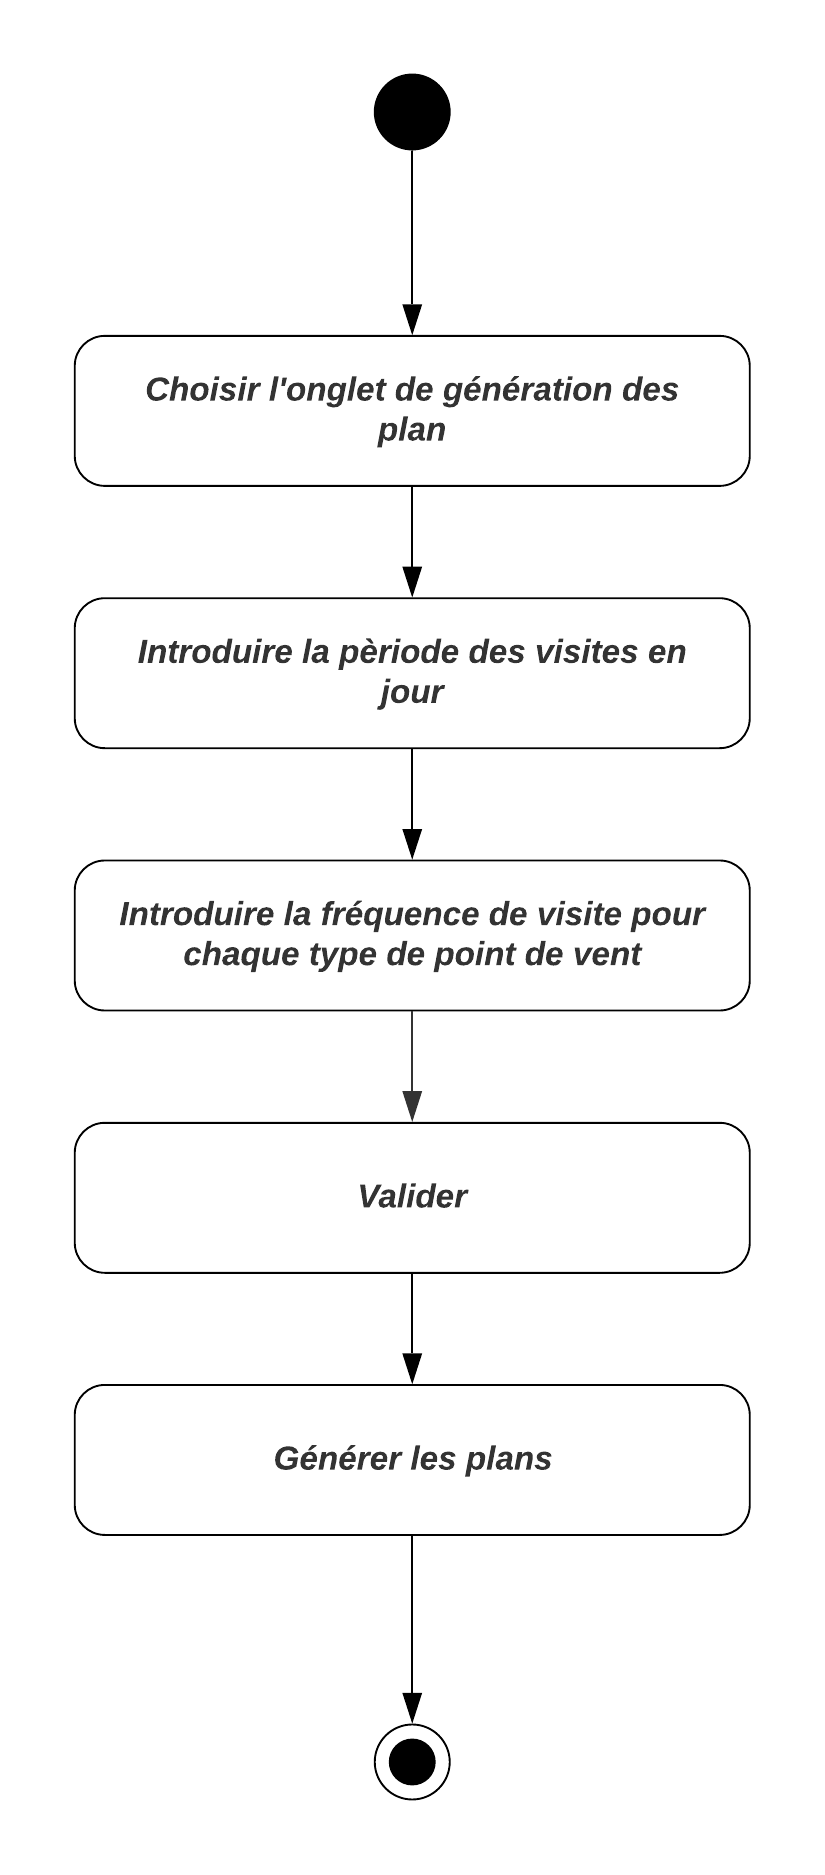
\includegraphics[height=17cm]{images_pfe/GENERATE_PLANS_DIAGRAM.png}
  \caption{Diagramme d'activité du CU: Générer les plans de visite des animateurs.}
  \label{fig:activity-admin}
\end{figure}
\FloatBarrier

\clearpage

\subsection{Animateur}


\begin{figure}[hbt!]
  \centering
  \includegraphics[width=\linewidth]{images_pfe/DCU_ANIMATEUR.png}
  \caption{Diagramme des cas d'utilisation de l'animateur.}
  \label{fig:dcu-animateur}
\end{figure}
\FloatBarrier

\renewcommand{\arraystretch}{1.5}
\begin{xltabular}{\linewidth}{|c|X|c|c|}
    \hline
    ID & CU & Documentation & Diagramme d'activité     \\\hline
    1 & S'authentifier & & \\ \hline
    10 & Récupérer les plans de visite & \checkmark & \\ \hline
    11 & Synchroniser les tournées & \checkmark & \checkmark \\ \hline
    12 & Visualiser les plans de route & & \\ \hline
    
    \caption{Liste des cas d'utilisation de l'animateur.}
    \label{tab:animator-use-cases}
\end{xltabular}
\FloatBarrier

\renewcommand{\arraystretch}{1.5}
\begin{xltabular}{\linewidth}{|X|}
    \hline
    \textbf{CU} : Récupérer les plans de visite    \\\hline
    \textbf{ID} :  10    \\\hline
    \textbf{Description brève} : Récupérer les plans de visite de l'animateur de pendant toute la période     \\\hline
    \textbf{Acteurs primaires} :   Animateur   \\\hline
    \textbf{Acteurs secondaires} : /     \\\hline
    \textbf{Pré condition} : L'animateur est déjà connecté   \\\hline
    \textbf{Enchaînement principal} : \\
    Le cas d'utilisation démarre lorsque l'animateur souhaite récupérer ses plans de visite.\\
    1. L'animateur choisit l'onglet plans de visite.\\
    2. Il lance la requête de récupération.\\
    3. Le système renvoie les plans de l'animateur.
    \\\hline
    \textbf{Post condition} :  Les plans de visite de l'animateur sont récupérés    \\\hline
    \textbf{Enchaînement alternatif} :  /   \\\hline
    
    \caption{Documentation CU : Récupérer les plans de visite.}
    \label{tab:cu-specs4}
\end{xltabular}
\FloatBarrier


\renewcommand{\arraystretch}{1.5}
\begin{xltabular}{\linewidth}{|X|}
    \hline
    \textbf{CU} : Synchroniser les tournées en temps réel     \\\hline
    \textbf{ID} :  11    \\\hline
    \textbf{Description brève} :  Mettre à jour la tournée par rapport à la fluidité du trafic routier    \\\hline
    \textbf{Acteurs primaires} :  Animateur    \\\hline
    \textbf{Acteurs secondaires} :   /   \\\hline
    \textbf{Pré condition} :   L'animateur est connecté   \\\hline
    \textbf{Enchaînement principal} :   \\
    Le cas d'utilisation démarre lorsque l'animateur souhaite synchroniser sa tournée.\\
    1. L'animateur choisit la section de synchronisation.\\
    2. L'animateur lance la requête de synchronisation.\\
    3. Le système renvoie la tournée synchronisée.
    \\\hline
    \textbf{Post condition} :  La tournée est synchronisée    \\\hline
    \textbf{Enchaînement alternatif} :  /    \\\hline
    
    \caption{Documentation CU : Synchroniser les tournées en temps réel.}
    \label{tab:cu-specs5}
\end{xltabular}
\FloatBarrier

\begin{figure}[hbt!]
  \centering
  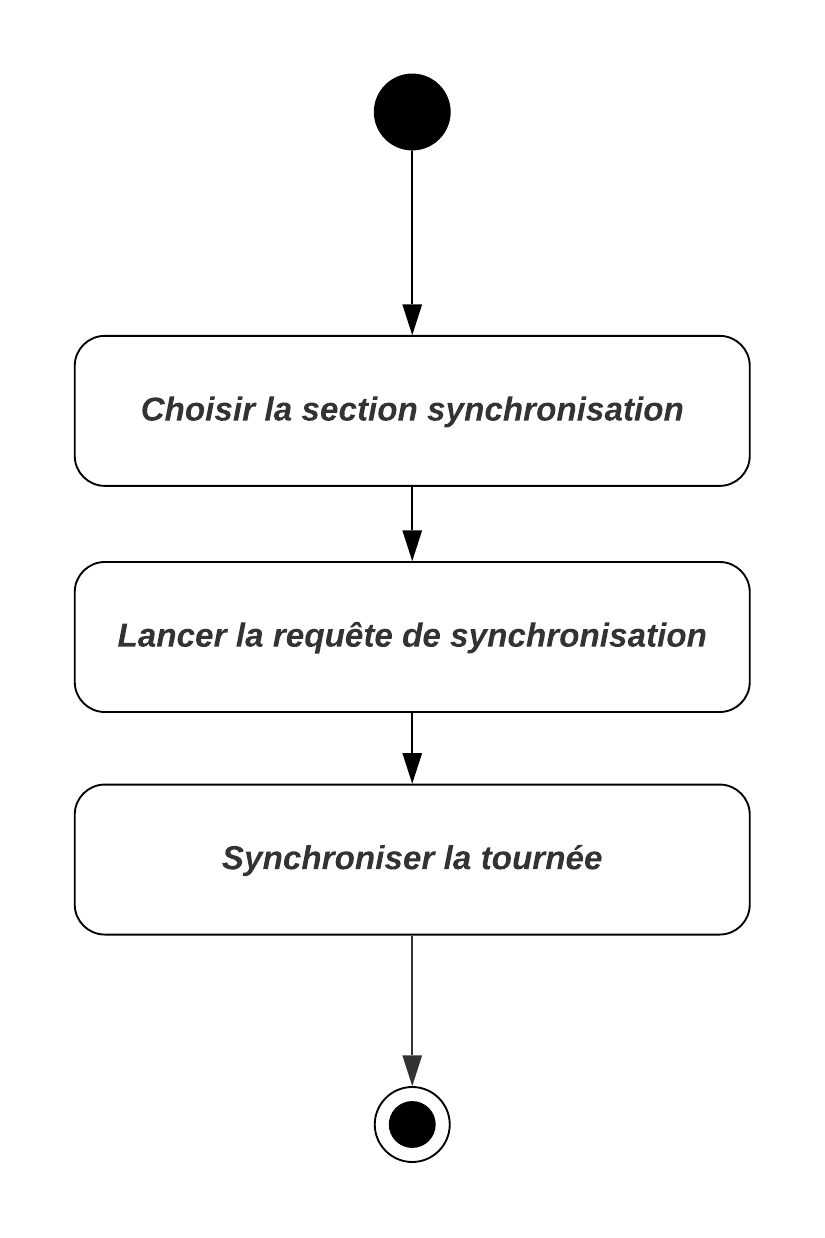
\includegraphics[height=13cm]{images_pfe/SYNC_TOUR_DIAGRAM.png}
  \caption{Diagramme d'activité du CU: Synchroniser les tournées en temps réel.}
  \label{fig:activity-animator}
\end{figure}
\FloatBarrier


\section{Conclusion}
Lorem ipsum dolor sit amet, consectetur adipiscing elit. Proin posuere euismod neque, non semper nibh viverra sed. Praesent ut varius magna. Fusce ipsum ante, semper nec interdum at, semper et lacus. Nulla ultrices magna a fringilla finibus. Etiam sollicitudin blandit ante. Vivamus blandit rhoncus tincidunt. Morbi sit amet congue purus. Praesent interdum gravida congue. Donec fermentum dui fermentum maximus rutrum.




%%% Local Variabs prles: 
%%% mode: latex
%%% TeX-master: "isae-report-template"
%%% End: 
\part{Contribution}

\chapter{Conception}

%\newpage

\section{Introduction}
Le domaine de l'apprentissage profond a connu une grande croissance de la profondeur des architectures de réseaux de neurones. Cependant, cette croissante pose des défis importants en termes d'exigences de calcul et mémoire et de consommation d'énergie. Ainsi, la nécessité de concevoir des techniques efficaces de compression et d'optimisation des modèles est devenue primordiale. Dans ce chapitre, nous présenterons une méthode automatique pour l'elagage des réseaux neuronaux très profonds qui exploite l'apprentissage par renforcement et le plongement des couches du réseau.

\section{Vue globale de la solution}
L'élagage des réseaux de neurones profonds est devenu une technique essentielle afin de déployer ces réseaux sur des appareils mobiles disposant de ressources de calcul et de stockage limitées. Plusieurs techniques existent pour élaguer un réseau. Cependant, ces techniques nécessitent des experts du domaine afin d'explorer le vaste espace de conception et obtenir un bon compromis entre la taille, la vitesse et la précision du modèle, ce qui peut prendre beaucoup de temps et ne produit pas toujours des résultats optimals.

Dans cette partie, nous proposons une nouvelle méthode d'élagage automatique des réseaux de neurones profonds qui utilise l'apprentissage par renforcement et les technique de plongement pour fournir les pourcentages d'élagage optimals. Notre méthode, contrairement aux méthodes conventionnelles, ne nécessite pas d'experts humains dans le domaine et prend moins de temps.

Dans les réseaux de neurones profonds, les couches ne sont pas indépendantes les unes des autres en raison de la manière dont l'information est propagée et traitée à travers le réseau. Chaque couche prend les sorties de la couche précédente en entrée et génère des sorties qui sont ensuite utilisées comme entrées pour la couche suivante. Cette interconnexion crée des relations et des dépendances entre les couches.

Lors de l'apprentissage, les poids et les biais de chaque couche sont ajustés et chaque couche contribue de manière spécifique à la transformation des données en fonction des poids et des biais. Donc, les ajustements dans une couche peuvent avoir un impact sur les performances et les caractéristiques apprises par les autres couches, et cela affecte directement la précision de notre modèle. Pour cela, nous avons décider d'utiliser une stratégie d'élagage continue. Nous commençons par l'initialisation des paramètres de notre modèle avec des valeurs aléatoires et puis nous entraînons le modèle jusqu’à l'obtention d'une bonne précision. Ensuite, nous commençons le processus d'élagage où nous utilisons un agent DDPG pour élaguer le réseau couche par couche (comme illustrée dans la figure \ref{fig:global-solution}). Pour chaque couche $L_n$ , l'agent DDPG reçoit comme entrée le plongement de la couche qui permet de préserver les caractéristiques utiles de cette couche, puis il génère en sortie un taux d'élagage $a_n$. Après l'élagage de la couche $L_n$ avec le taux $a_n$, l'agent DDPG passe à la couche suivante $L_{n+1}$.

\begin{figure}[hbt!]
  \centering
  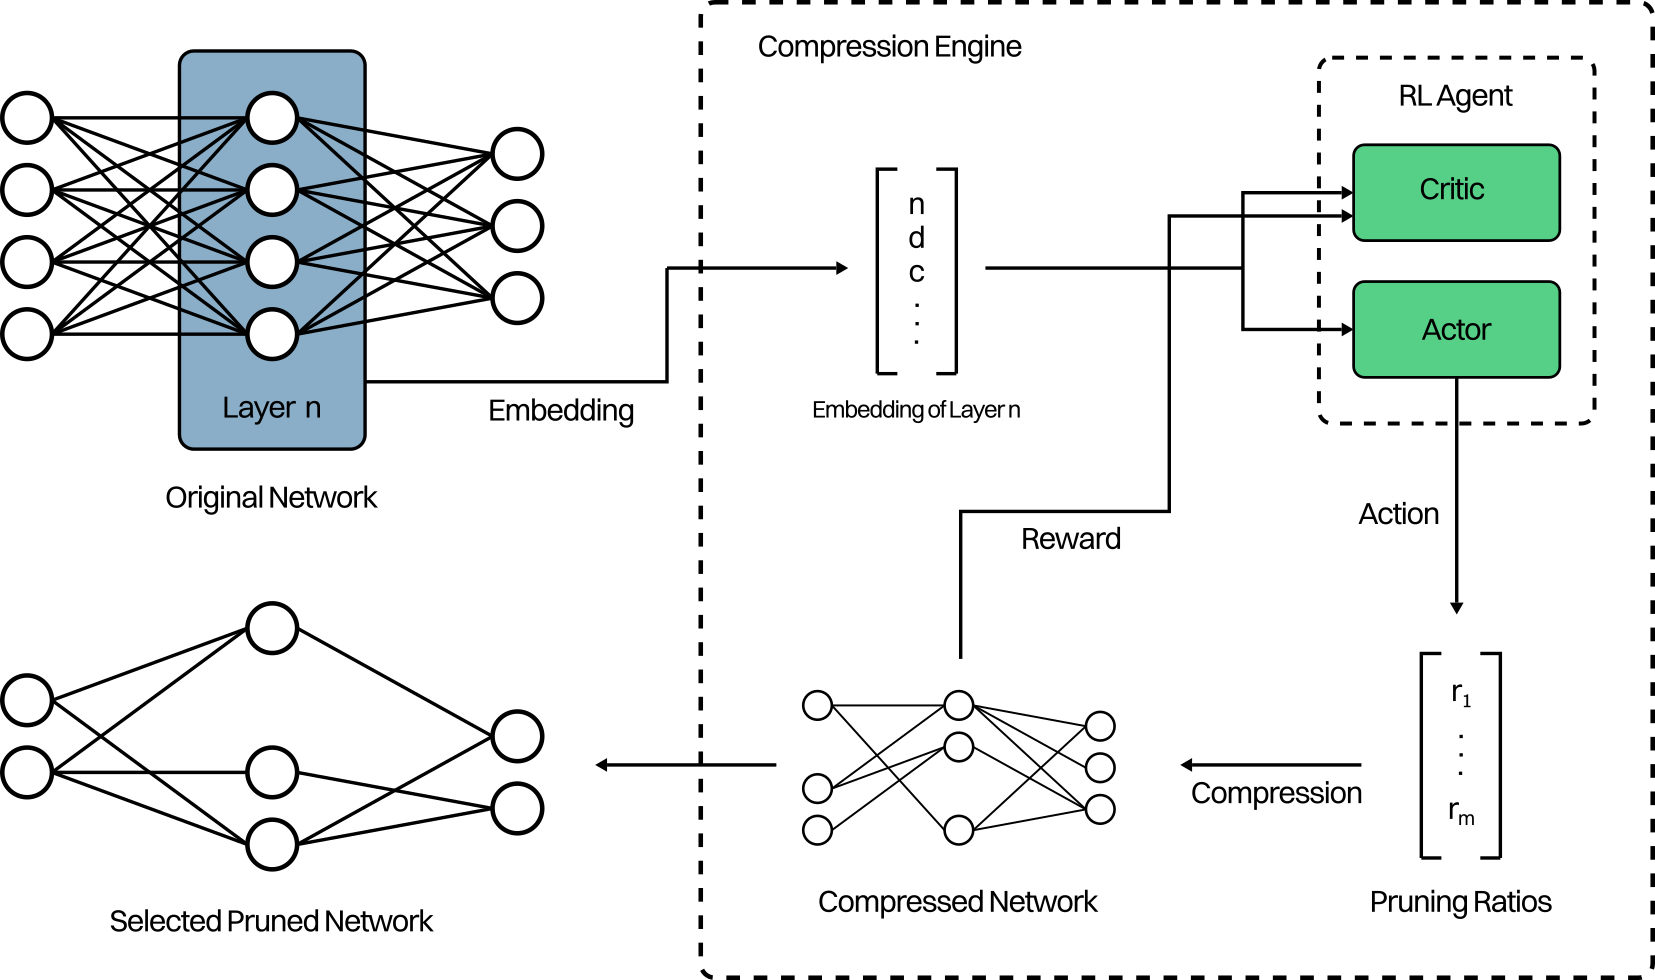
\includegraphics[width=14cm]{images_pfe/global-solution.png}
  \caption{Présentation du processus d'élagage.}
  \label{fig:global-solution}
\end{figure}
\FloatBarrier
\medskip


Une fois toutes les couches élaguées, nous évaluons la précision du modèle sans réglage fin afin d'estimer la précision du modèle final (avec le réglage fin). Cette valeur approchée permet d'améliorer le temps de recherche sans avoir à ré-entraîner le modèle à chaque fois. Une fois la recherche terminée, nous effectuons un réglage fin au modèle avec la meilleure précision pour améliorer encore sa précision.

Généralement, nous pouvons décomposer le processus d'élagage en 4 étapes principales (comme illustré dans la figure \ref{fig:global-schema}):
\begin{enumerate}
    \item \textbf{Initialisation}: Nous commençons par le définition du modèle et l'initialisation aléatoire de ses paramètres.
    \item \textbf{Entraînement}: Nous entraînons le modèle à l'aide du jeu de données CIFAR-10 jusqu'à ce que nous obtenions la meilleure précision.
    \item \textbf{Élagage}: Nous utilisons l'agent DDPG pour fournir les pourcentages d'élagage de chaque couche, et nous sélectionnons le meilleure réseau parmi les réseaux élagués pour l'améliorer dans l'étape suivante.
    \item \textbf{Réglage fin}: Nous ré-entraînons le réseau obtenu dans l'étape précédente pour améliorer encore sa précision.
\end{enumerate}

\begin{figure}[hbt!]
  \centering
  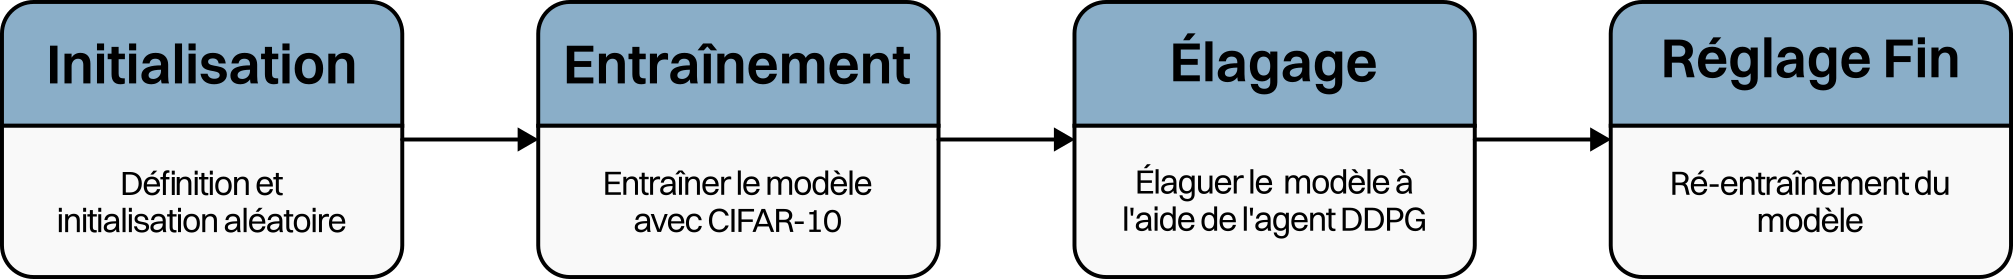
\includegraphics[width=14cm]{images_pfe/schema-general.png}
  \caption{Schéma global du processus d'élagage.}
  \label{fig:global-schema}
\end{figure}
\FloatBarrier
\medskip

\section{Plongements des couches}
Il existe plusieurs architectures de réseaux de neurones et les couches et les connexions entre elles diffèrent d’une architecture à l’autre. Dans ce travail, nous allons concentrer uniquement sur les réseaux de neurones de convolution et résiduels, qui utilisent deux types de couches seulement: les couches de convolution et les couches entièrement connectées.

Comme illustrée dans la figure \ref{fig:global-solution}, l'agent DDPG reçoit le plongement de la couche $L_n$ en entrée et fournit en sortie le taux d'élagage $a_n$ de cette couche. La raison derrière l'utilisation du plongement de couche au lieu du plongement d'un graphe de calcul avec encodeur GCN (qui est utilisé dans la méthode de \cite{pfe2022}) est que le plongement de couche est généralement plus simple à mettre en œuvre et plus rapide.

D'une part, le plongement de couche peut simplifier la représentation d'entrée et réduire la dimensionnalité par rapport à une représentation graphique, ce qui rend les données plus faciles à traiter et l'apprentissage plus rapide. D'autre part, lors de l'utilisation du graphe de calcul avec GCN, la construction et reconstruction du graphe entraînent une surcharge à chaque étape de l'apprentissage par renforcement. Nous devons toujours reconstruire le graphe de calcul en fonction du taux d'élagage actuel, ce qui peut être coûteux en termes de calculs et peut ralentir le processus d'élagage, tandis que dans les plongements de couches, nous trouvons qu'ils sont plus interprétables et nécessitent moins d'efforts pour les construire, visualiser et comprendre par rapport aux structures graphiques. Finalement, la complexité des méthodes basées sur GCN peut augmenter considérablement lorsque la taille du réseau de neurones augmente, ce qui n'est pas le cas pour les plongement de couches car ils sont plus évolutives et fonctionnent mieux dans des environnements à grande échelle.

Chaque plongemenet $s_n$ est caractérisé par 11 caractéristiques qui sont essentielles pour que l’agent DDPG puisse distinguer une couche d’une autre. Ces caractéristiques sont les suivantes:
\begin{equation}
    (n, d, c, h, w, stride, k, FLOPs[n], removed, remaining, a_{n−1} )
\end{equation}
où:
\begin{conditions}
    n & L'indice de la couche\\
    d et c & Les canaux de sortie et d'entrée\\
    h & Le nombre de pixels dans la direction verticale\\
    w & Le nombre de pixels dans la direction horizontale\\
    stride & La taille du pas du filtre\\
    k & La taille du noyau\\
    FLOPs[n] & Les FLOPs de la couche $L_n$\\
    removed & Le nombre total de FLOPs supprimés dans les couches précédentes\\
    remaining & Le nombre de FLOPs restants dans les couches suivantes\\
    a_{n-1} & Le taux d'élagage de la couche précédente\\
\end{conditions}
% \begin{itemize}
%     \item \textit{n}: L'indice de la couche
%     \item \textit{d} et \textit{c}: Les canaux de sortie et d'entrée
%     \item \textit{h}: Le nombre de pixels dans la direction verticale
%     \item \textit{w}: Le nombre de pixels dans la direction horizontale
%     \item \textit{stride}: La taille du pas du filtre
%     \item \textit{k}: La taille du noyau
%     \item \textit{FLOPs[n]}: Les FLOPs de la couche $L_n$
%     \item \textit{removed}: Le nombre total de FLOPs supprimés dans les couches précédentes
%     \item \textit{remaining}: Le nombre de FLOPs restants dans les couches suivantes
%     \item $a_{n-1}$: Le taux d'élagage de la couche précédente
% \end{itemize}

Après l'extraction de ces caractéristiques, nous effectuons une normalisation afin de les préparer à être utilisées comme entrées dans l'agent DDPG. La normalisation garantit que les valeurs des caractéristiques extraites se situent dans une plage similaire. Ceci est important pour la stabilité de l'entraînement et la convergence de l’agent DDPG. Il existe plusieurs méthodes pour faire la normalisation telles que:
\begin{itemize}
    \item \textbf{Min-Max scaling}: Cette méthode transforme les valeurs des caractéristiques en une plage prédéfinie, souvent [0, 1] ou [-1, 1]. Il faut d'abord Identifier les valeurs minimales et maximales de la caractéristique, puis soustrayez la valeur minimale et divisez par la plage (maximum moins minimum) pour chaque valeur de la caractéristique.
    \item \textbf{Z-Score (standardisation)}: Cette méthode met à l'échelle les valeurs pour avoir une moyenne de 0 et un écart type de 1. D'abord, on calcule la moyenne et l’écart type de la caractéristique. Puis, pour chaque valeur de la caractéristique, on soustrait la moyenne et on divise par l'écart type.
    \item \textbf{Feature Scaling}: Avec cette méthode, on met à l'échelle chaque caractéristique individuellement pour avoir une moyenne de 0 et une variance de 1. Ceci peut être réalisé en soustrayant la moyenne et en divisant par l'écart type pour chaque caractéristique séparément.
\end{itemize}

Dans notre cas, nous allons utiliser la méthode Min-Max scaling pour garantir que toutes les valeurs sont ajustées proportionnellement pour s'adapter à la plage [0, 1].

\section{Choix des pourcentages d'élagage}
Afin de choisir les meilleurs pourcentages d'élagage, nous disposons de certaines métriques qui guident ce processus. Ces métriques sont essentielles pour l'évaluation des performances des réseaux de neurones élagués. Les métriques que nous examinerons comprennent le temps d'inférence et la taille du réseau.

Le temps d'inférence est une mesure du délai nécessaire pour obtenir une sortie suite à la présentation d'une entrée au réseau, c'est à dire c'est le temps nécessaire pour faire une propagation vers l'avant. Une diminution de ce temps se traduit par une amélioration de la réactivité globale du réseau. De plus, la réduction de la taille du réseau apporte plus d'avantages, allant de la réduction des besoins en espace de stockage à une consommation énergétique réduite.

Cependant, ces deux métriques sont liées à un paramètre important: le degré de sparsité du réseau, qui, lorsqu'il augmente, il peut engendrer des gains significatifs en termes de taille du réseau et de rapidité d'inférence. Ce paramètre mesure la proportion de paramètres qui ont été élagués par rapport au nombre total de paramètres dans le modèle d'origine. Toutefois, nous pouvons avoir une perte de performances du modèle lorsque nous augmentons extrêmement le degré de sparsité du réseau. Il est donc nécessaire de trouver un équilibre entre la réduction de la taille et le maintien des performances.

Pour augmenter le degré de sparsité du réseau, nous devons réduire/augmenter l'une des 4 mesures suivantes: les paramètres du réseau, les FLOPs, les FLOPS, ou les MAC.

\subsubsection{Paramètres}
Les paramètres font référence aux poids et aux biais qui sont ajustés pendant l'entraînement du réseau. Chaque connexion entre les neurones est associée à un poids, qui détermine l'importance de cette connexion pour le calcul de la sortie. En ajustant ces poids et biais lors de la phase d'entraînement, le réseau apprend à représenter les relations entre les entrées et les sorties. Le nombre total de paramètres dans un réseau est un facteur crucial qui, avec son augmentation, peut rendre le réseau plus grand en termes de taille et complexe à entraîner.

Prenons l'exemple d'un réseau de neurones convolutionnel (CNN). Chaque couche de ce réseau contient des filtres qui glissent sur l'image d'entrée pour extraire des caractéristiques. Chaque connexion entre un filtre et une région de l'image a un poids associé. Ces poids constituent les paramètres du réseau. Par exemple, si nous avons un filtre de taille 3x3, il y aura 9 poids (un pour chaque connexion) et un biais associé à ce filtre. Si le réseau a plusieurs de ces filtres dans une couche, le nombre total de paramètres augmentera en conséquence.

\subsubsection{FLOPs}
Les FLOPs (Floating Point Operations) sont une mesure du nombre total des opérations en virgule flottante effectués par le modèle, telles que les additions, les soustractions, les multiplications et les divisions. Un modèle avec un grand nombre de FLOPs peut nécessiter plus de ressources de calcul et de temps pour l'entraînement et l'inférence.

Souvent, le nombre de paramètres est utilisé pour mesurer la complexité du modèle, mais il ne se traduit pas directement en charge computationnelle lors de l'inférence. Dans ce travail, nous allons utiliser les FLOPs comme critère de choix des pourcentage d’élagage au lieu d'utiliser les paramètres. Les raisons de ce choix sont citées dans la section suivante.

\subsubsection{FLOPS}
Les FLOPS (Floating Point Operations per Second) sont le nombre d'opérations en virgule flottante qui peut être effectuer par seconde et ils sont utilisés pour évaluer la capacité de calcul et les performances d'un dispositif ou des unités de traitement, telles que les processeurs et les GPU. Plus le nombre de FLOPS est élevé, plus le dispositif est capable de réaliser des calculs complexes rapidement et l’inférence sera plus rapide.

Par exemple, pour une carte graphique (GPU) qui a une capacité de calcul de 10 téraflops ($10 \cdot 10^{12} FLOPS$), elle peut effectuer environ 10 billions d'opérations en virgule flottante par seconde. Cela serait particulièrement utile pour accélérer l'entraînement des réseaux très profonds.

\subsubsection{MAC}
Un MAC (Multiply-Accumulate Computations) combine une multiplication suivie d'une addition de produits résultants. Il est utilisé pour calculer les sorties des neurones en multipliant les entrées par les poids associés, puis en accumulant ces produits pour obtenir la sortie finale du neurone. Généralement, on considère 1 MAC = 2 FLOPs.

\subsection{Raisons d'utilisation des FLOPs}
Dans les réseaux CNN, la réduction du nombre de paramètres ne se traduit pas nécessairement par une réduction proportionnelle en termes d'opérations en virgule flottante (FLOPs). Ces dernières dépendent de plusieurs facteurs au-delà du simple nombre de paramètres, tels que:
\begin{itemize}
    \item \textbf{Taille des filtres}: La taille des filtres de convolution affecte le nombre de calculs. Les filtres plus grands nécessitent plus de calculs par couche.
    \item \textbf{Taille de l'entrée}: La taille de l'entrée d'une couche affecte également le nombre de calculs. Des dimensions d'entrée plus grandes nécessitent plus de calculs pour être traitées.
    \item \textbf{Stride}: Le stride (pas) détermine comment les filtres de convolution se déplacent à travers les données d'entrée. Les pas plus grands réduisent le nombre de calculs, car ils sautent certaines régions de l'entrée.
    \item \textbf{Pooling}: Les couches de regroupement maximal (maxpool) ou de regroupement moyen (avgpool) sont utilisées dans les CNN pour réduire les dimensions spatiales. Ces couches affectent également la charge de calcul globale.
    \item \textbf{Non-linéarité}: Les fonctions d'activation telles que ReLU introduisent des calculs supplémentaires lors des passes avant et arrière.
    \item \textbf{Connexions sautées et blocs résiduels}: Les connexions sautées ou les blocs résiduels peuvent introduire des calculs supplémentaires.
\end{itemize}

Prenons un exemple simple avec deux couches de convolution dans le réseau. Supposons que les deux couches ont le le même filtre et stride mais la première couche possède une entrée plus grande que la deuxième, c'est a dire que la deuxième couche nécessitera moins de FLOPs par rapport à la première couche. Nous avons donc deux scénarios: 
\begin{enumerate}
    \item \textbf{Élagage en pourcentage de paramètres}: Dans ce scénario, si on élague 25\% de la première couche et 75\% de la deuxième couche, on va élaguer donc 50\% des paramètres ($\frac{25+75}{2}$). Cela réduit le nombre total de paramètres, mais ne correspond pas nécessairement à une réduction proportionnelle des calculs car la première couche a plus de calculs que la deuxième couche (la réduction des FLOPs pourrait être bien inférieure à 50\%).
    \item \textbf{Élagage en pourcentage de FLOPs}: Contrairement à la réduction de paramètres, si on élague 50\% de FLOPs, alors on va élaguer 50\% des calculs, ce qui est plus avantageux.
\end{enumerate}

\subsection{Calcul des FLOPs}
Comme indiqué précédemment, le nombre des FLOPs peut être influencé par plusieurs facteurs, tels que la taille d'entrée, le stride, la taille du filtre, etc. L'estimation du nombre de FLOPs ne tient peut-être pas compte de toutes les complexités des opérations spécialisées, des optimisations matérielles et des détails d'implémentation, mais elle fournit une estimation approximative de la complexité de notre modèle.

Pour calculer le nombre des FLOPs dans un modèle, nous avons des règles différentes pour chaque type de couche:
\begin{itemize}
    \item \textbf{Couche de convolution} \begin{equation}
        FLOPs = 2 \cdot C_I \cdot C_O \cdot K \cdot O
    \end{equation}
    \item \textbf{Couche entièrement connectée} \begin{equation}
        FLOPs = 2 \cdot I \cdot O
    \end{equation}
\end{itemize}

où:
\begin{conditions}
    C_I & Le nombre de canaux d'entrée\\
    C_O & Le nombre de canaux de sortie\\
    K & La forme du noyau\\
    I & La taille de l'entrée\\
    O & La taille de la sortie\\
\end{conditions}
% \begin{itemize}
%     \item $C_I$: Le nombre de canaux d'entrée
%     \item $C_O$: Le nombre de canaux de sortie
%     \item \textit{K}: La forme du noyau
%     \item \textit{I}: La taille de l'entrée
%     \item \textit{O}: La taille de la sortie
% \end{itemize}

Supposons que nous avons le modèle suivant qui effectue une classification sur le jeu de données MNIST, où:
\begin{itemize}
    \item La taille de l'entrée est 28x28x1 (niveaux de gris)
    \item Nous commençons par 2 convolutions de 5 noyaux de taille (3x3)
    \item Nous exécutons ensuite une couche entièrement connectée de 128 neurones
    \item Nous terminons avec une couche entièrement connectée de 10 neurones
\end{itemize}

Donc, le nombre de FLOPs pour les 4 couches de notre modèle est calculé comme suit:
\begin{itemize}
    \item \textbf{Première convolution}: $2 × 1 × 5 × (3 × 3) × 26 × 26 = 60 840 FLOPs$
    \item \textbf{Deuxième convolution}: $2 × 5 × 5 × (3 × 3) × 24 × 24 = 259 200 FLOPs$
    \item \textbf{Première couche FC}: $2 × (24 × 24 × 5) × 128 = 737 280 FLOPs$
    \item \textbf{Deuxième couche FC}: $2 × 128 × 10 = 2 560 FLOPs$
\end{itemize}
Le modèle fera donc  $60 840 + 259 200 + 737 280 + 2 560 = 1 060 400$ opérations.

\begin{figure}[hbt!]
  \centering
  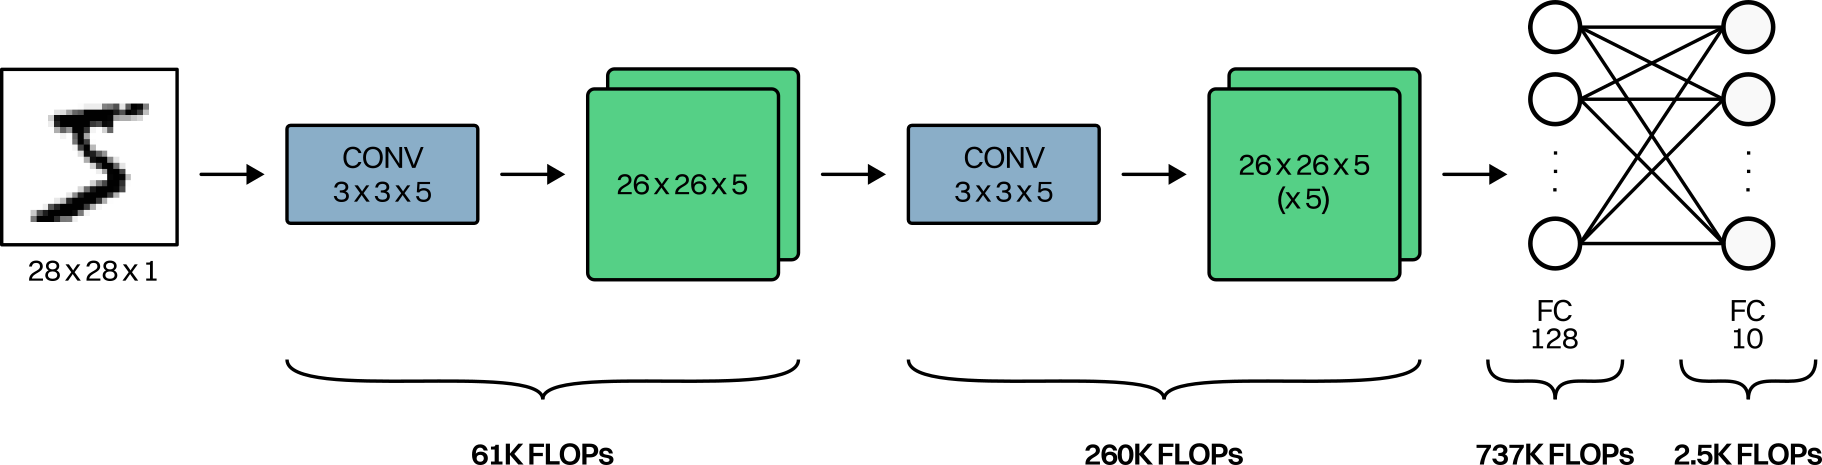
\includegraphics[width=15cm]{images_pfe/mnist.png}
  \caption{Nombre des FLOPs dans le modèle.}
  \label{fig:mnist}
\end{figure}
\FloatBarrier
\medskip

\section{Choix du type d'élagage}
Lors de la conception de notre méthode d'élagage, le choix entre l'élagage structuré et non structuré a été une considération essentielle. L'élagage structuré cible des motifs spécifiques, tels que des neurones entiers, des canaux ou des couches, tandis que l'élagage non structuré élimine des poids individuels sans tenir compte de leur emplacement dans le réseau. Chaque approche offre des avantages distincts et des compromis, influençant leur pertinence pour différentes situations d'élagage. Dans cet section, nous explorons les deux types d'élagage et nous sélectionnons un pour l'utiliser dans notre travail.

L'élagage structurée consiste à supprimer des unités ou blocs entiers du réseau de neurones, tels que des filtres, des canaux (plusieurs filtres) ou des couches entières, tout en conservant l'architecture globale du réseau. Cela permet d'avoir une compression plus importante de notre modèle car des structures entières sont supprimées, ce qui peut conduire à un déploiement très efficace sur des appareils avec des ressources de calculs et de stockage limitées. Cependant, l'élagage structuré peut affecter négativement la précision du réseau puisque certains poids importants peuvent être éliminés, et il pourrait nécessiter un ajustement fin pour récupérer les performances perdues.

D'autre part, l'élagage non structuré permet de supprimer des poids individuels ou des connexions du réseau, ce qui permet potentiellement de mieux conserver la précision. Toutefois, il ne conduit pas toujours à des gains significatifs en termes de mémoire et de temps d'inférence puisque le nombre de calculs reste le même (nous avons le même nombre de filtres et les poids éliminés sont seulement remplacés pare des zéros).

Le choix entre ces deux techniques dépend de facteurs tels que l'architecture spécifique du réseau, le matériel disponible et le compromis souhaité entre la compression et les performances. Dans notre cas, nous souhaitons déployer les modèles élagués dans des appareils avec des ressources limitées, c'est pourquoi d'élagage structuré est la meilleure approche à utiliser. Nous utilisons la norme L1 pour identifier et supprimer les canaux les moins importants. La norme L1 est simplement la somme des valeurs absolues des poids $|w_i|$ du canal (\ref{equ:l1}). Pour chaque canal, la norme L1 des poids du canal est calculée et les canaux avec des valeurs plus faibles sont considérés comme moins importants et sont sélectionnés puis supprimés de la couche de convolution.

\begin{equation}
    L1 Norm = \sum |w_i|
    \label{equ:l1}
\end{equation}

\begin{figure}[hbt!]
  \centering
  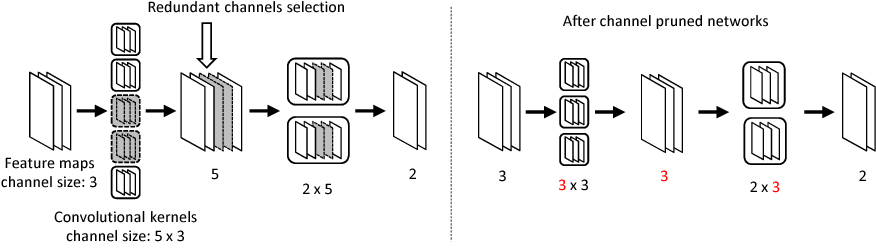
\includegraphics[width=15cm]{images_pfe/channel-pruning.png}
  \caption{Illustration du mécanisme d’élagage des canaux [\cite{Yamamoto2018PCASPC}].}
  \label{fig:mnist}
\end{figure}
\FloatBarrier
\medskip

Après avoir retiré les canaux, le réseau peut subir un ajustement (ré-entraînement) pour rétablir les performances perdues. Cela peut impliquer l'entraînement du réseau élagué, en gardant les valeurs finales des poids après l'élagage, avec un taux d'apprentissage plus petit sur les exemples d'entraînement restants.

\section{Implémentation de l’apprentissage par renforcement}
Comme illustré sur la figure \ref{fig:global-solution}, l'agent reçoit le plongement $s_n$ de la couche $L_n$, puis génère un pourcentage d'élagage de cette couche en tant qu'action $a_n$. Ensuite, La couche $L_n$ est élaguée avec le pourcentage $a_n$ à l'aide de algorithme d'élagage de canaux. Après l'élagage de la couche $L_n$, l'agent passe à la couche suivante $L_{n+1}$ et reçoit son plongement $s_{n+1}$ en entrée. Après avoir élagué toutes les couches, la récompense est évaluée puis renvoyée à l'agent. Dans cette section, nous allons présenter en détail la théorie et l'implémentation de l'algorithme Deep Deterministic Policy Gradient (DDPG) dans notre méthode d'élagage automatique. Nous avons choisi d'utiliser DDPG au lieu de PPO (qui est utilisé dans la méthode présentée par \cite{pfe2022}) parceque DDPG a tendance à converger plus rapidement que PPO dans de nombreux cas. Cette vitesse de convergence est attribuée en partie au fait que DDPG utilise des politiques déterministes et PPO utilise des politiques stochastiques, c'est-à-dire qu'à chaque étape, l'agent DDPG choisit une action spécifique sans aucune composante aléatoire, tandis que l'agent PPO choisit une action avec une composante aléatoire. Cette stochasticité peut ralentir la convergence de l'agent PPO car il doit explorer différentes actions pour déterminer quelle est la meilleure.


\subsection{Agent DDPG}
Dans l'apprentissage par renforcement, les algorithmes de gradient de politique sont utilisés avec une fonction de politique stochastique $\pi(s)$. Cela signifie que, pour un état donné, il y aura une distribution de probabilité pour chaque action dans l’espace d’action. Dans le cas de l'algorithme DDPG (Deep Deterministic Policy Gradient), on utilise une politique déterministe $\mu(s)$ au lieu de la politique stochastique $\pi(s)$. Pour un état \textit{s} donné, il y aura une décision déterministe $\mu(s)$ au lieu d'une distribution sur les actions.

Cet algorithme (DDPG) est un algorithme acteur-critique hors politique (off-policy) qui vise à résoudre des problèmes de contrôle continu, où les actions à prendre sont des valeurs continues plutôt que discrètes. Cet algorithm est une extension de l'apprentissage Q profond et l'algorithme DPG (Deterministic Policy Gradient) qui intègre des réseaux de neurones profonds pour mieux gérer les espaces d'actions et d'états complexes. L'apprentissage Q profond fonctionne dans un espace d'action discret et le DPG l'étend à l'espace d'action continu tout en apprenant une politique déterministe. Donc, Il apprend simultanément une fonction \textit{Q} et une politique déterministe où il utilise des données hors politique et l'équation de Bellman (\ref{equ:bellman}) pour apprendre la fonction \textit{Q}, et puis il utilise la fonction \textit{Q} pour apprendre la politique.

\begin{figure}[hbt!]
  \centering
  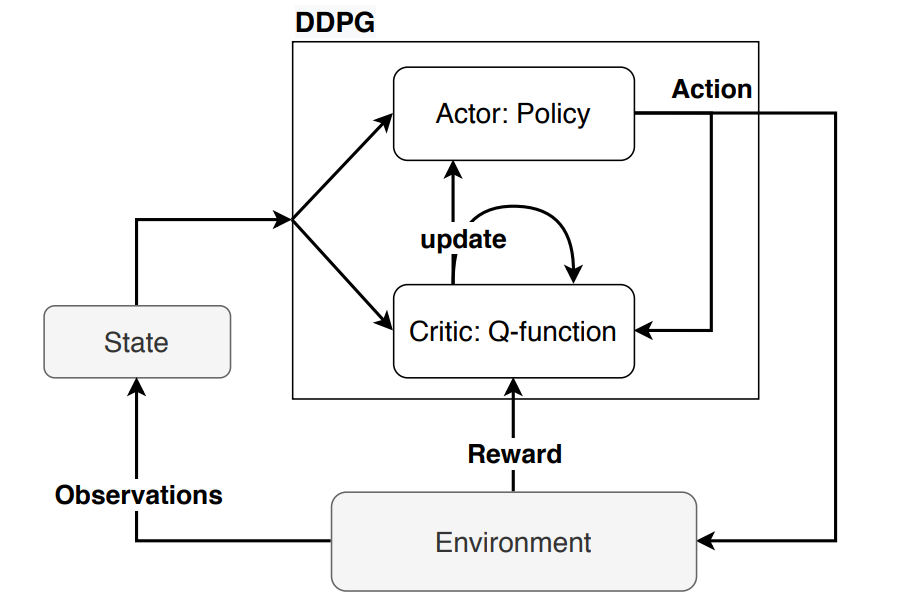
\includegraphics[width=15cm]{images_pfe/ddpg-overview.png}
  \caption{Schéma de présentation de l'algorithme DDPG [\cite{handaoui2020releaser}].}
  \label{fig:ddpg-overview}
\end{figure}
\FloatBarrier
\medskip

L'une des difficultés dans l'apprentissage par renforcement est l'exploration de l'espace d'actions pour découvrir de bonnes stratégies. Dans DDPG, on utilise une politique stochastique pour introduire de l'exploration où on ajoute un bruit additif dans les actions choisies par l'acteur. Dans notre travail, nous utilisons une distribution normale (politique gaussienne) pour le bruit additif (\ref{equ:gaussian-noise}).
\begin{equation}
    \mu^{'} (s_n) \sim N(\mu (s_n | \Theta_{n}^{\mu}), \sigma^2, 0, 1)
    \label{equ:gaussian-noise}
\end{equation}

Pendant l'exploitation, le bruit $\sigma$ est initialisé à 0,5 et diminué de façon exponentielle après chaque épisode. Pour une exploration rapide, nous calculons la récompense sans réglage fin pour avoir une bonne approximation de la précision après le réglage fin.

\subsubsection{Politique gaussienne}
Pour permettre à l'agent de découvrir de nouvelles stratégies potentiellement meilleures, nous allons ajouter du bruit gaussien aux actions choisies par le réseau d'acteur. Ce bruit, également appelé distribution normale ou bruit blanc, est une distribution de probabilité caractérisée par sa moyenne $\mu$ et son écart type $\sigma$. Le bruit ajouté à chaque action est tiré de cette distribution et il permet d'explorer différentes parties de l'espace des actions. La formule \ref{equ:gaussian-distribution} représente la fonction de la distribution gaussienne.
\begin{equation}
    f(x) = \frac{1}{\sigma \sqrt{2\pi}}e^{-\frac{1}{2}(\frac{x-\mu}{\sigma})^2}
    \label{equ:gaussian-distribution}
\end{equation}


Le degré d'exploration peut être contrôlé en ajustant les paramètres de la distribution gaussienne. Nous initialisons l'écart type à une valeur plus élevée (0,5 dans notre cas), ce qui entraîne plus d'exploration, car le bruit ajouté aux actions devient plus important et imprévisible. Après chaque épisode, nous allons diminuer sa valeur de façon exponentielle. Pour la moyenne $\mu$, elle peut être fixée à zéro ou à une petite valeur. Elle n'affecte pas significativement l'exploration, car elle décale le bruit seulement sans altérer son caractère aléatoire.

Ce bruit d'exploration équilibre le compromis entre l'exploration et l'exploitation. Au début, lorsque l'agent apprend, l'exploration est importante pour découvrir différentes actions. À mesure que l'entraînement progresse, le bruit sera progressivement réduit pour se concentrer davantage sur l'exploitation de la politique apprise. Pour ajouter ce bruit aux actions, nous utilisons un générateur de nombres aléatoires pour tirer des échantillons d'une distribution gaussienne

\begin{figure}[hbt!]
  \centering
  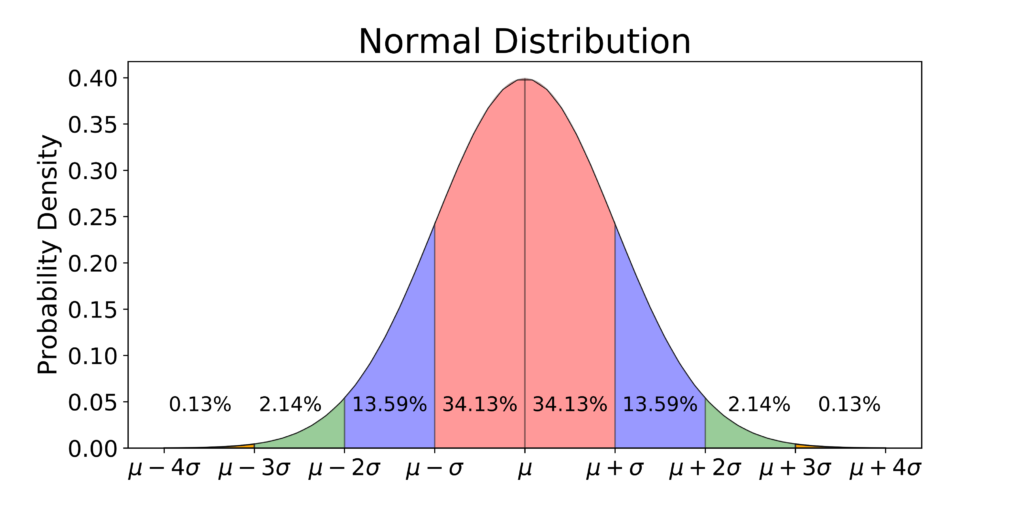
\includegraphics[width=15cm]{images_pfe/normal-distribution.png}
  \caption{Courbe de la distribution gaussienne [\cite{yoseph2019}].}
  \label{fig:normal-distribution}
\end{figure}
\FloatBarrier
\medskip

\subsection{Équations Clés}
\subsubsection{Valeur cible (Target Value) pour le Critique}
Le réseau de critique a pour objectif de minimiser l'écart entre la valeur prédite et la récompense réelle et estimer la récompense cumulative attendue pour une paire état-action donnée. La valeur cible $y_i$ pour le réseau de critique, qui est un élément crucial dans la mise à jour du réseau de critique, est calculée en fonction de la récompense immédiate $r_i$ reçue à l'instant \textit{i} de la valeur estimée de la prochaine paire état-action.
\begin{equation}
    y_i = r_i - b + \gamma \cdot Q(s_{i+1}, \mu (s_{i+1}) | \Theta^Q)
\end{equation}
où $Q(s_{i+1}, \mu (s_{i+1})$ représente la récompense cumulée estimée pour le prochain état $s_{i+1}$ et l'action proposée par le réseau d'acteurs cibles $\mu$, $\gamma$ représente le facteur de remise (discount factor), \textit{b} est la récompense de base et $\mu$ représente le réseau d'acteur cible qui donne l'action suggérée pour le prochain état. La récompense de base \textit{b} est soustraite pour réduire la variance de l'estimation du gradient, qui est une moyenne exponentielle des récompenses précédentes, tandis que le facteur de remise $\gamma$ est fixé à 1 pour éviter de donner la priorité aux récompenses à court terme.

\subsubsection{Mise à jour du Critique}
Le réseau de critique est mis à jour en minimisant la perte moyenne entre la valeur prédite $Q(s_i,a_i)$ et la valeur cible $y_i$. La perte \textit{L} est calculé pour chaque pas de temps, et le but est d'ajuster les paramètres du réseau critique pour minimiser cette perte. 
\begin{equation}
    L = \frac{1}{N}\sum_i(y_i - Q(s_i, a_i | \Theta^Q))^2
\end{equation}
Cette mise à jour aide le réseau critique à mieux se rapprocher de la véritable récompense cumulée attendue.

\subsubsection{Mise à jour de l'Acteur}
L'objectif de l'acteur est d'apprendre une politique qui maximise la récompense cumulée attendue telle qu'estimée par le réseau critique. En d'autres terms, il s'agit de maximiser les valeurs prédites du critique pour les actions prises. La mise à jour du réseau d'acteurs consiste à calculer le gradient de la récompense cumulée attendue par rapport aux paramètres de l'acteur $\Theta_\mu$. Ce gradient est approximé comme suit:
\begin{equation}
    \nabla_{\Theta_\mu}J \approx \mathbb{E}_{s_i}[\nabla_a Q(s_i, a) |_{a=\mu(s_i)} \nabla_{\Theta_\mu}\mu(s_i)]
\end{equation}

où \textit{J} est la fonction d'objectif de l'acteur, $\Theta_\mu$ sont les paramètres du réseau d'acteur, $\mu(s_i)$ est l'action produite par le réseau d'acteur pour l'état $s_i$ et $\nabla_a Q(s_i, a)$ représente le gradient de la valeur du critique par rapport à l'action.


La mise à jour des paramètres $\Theta_\mu$ de l'acteur est effectuée en utilisant ce gradient pour déplacer la politique dans la direction qui augmente la récompense cumulative attendue. La règle de mise à jour des paramètres de l'acteur est donnée par la formule \ref{equ:maj-parameters}.
\begin{equation}
    \Delta \Theta_\mu = \alpha \nabla_{\Theta_\mu}J
    \label{equ:maj-parameters}
\end{equation}
où $\alpha$ est le taux d'apprentissage.

\newcommand\mycommfont[1]{\footnotesize\ttfamily\textcolor{blue}{#1}}
\SetCommentSty{mycommfont}

\subsection{Acteur-Critique}
L'algorithme DDPG utilise deux types de réseaux de neurones profonds: un réseau d'acteur (Actor Network) et un réseau de critique (Critic Network).

\begin{figure}[hbt!]
  \centering
  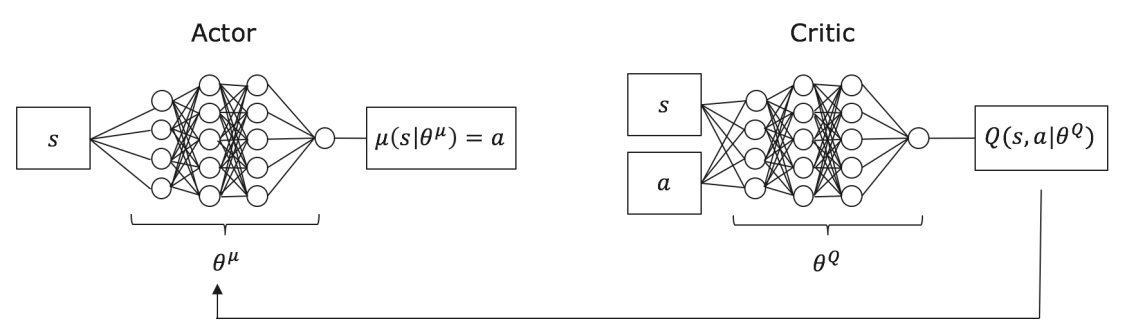
\includegraphics[width=15cm]{images_pfe/ddpg-actor-critic.png}
  \caption{Structure de base de l'agent acteur-critique DDPG. L'acteur prend l'état \textit{s} comme entrée et produit une action basée sur la politique déterministe $\mu$ comme résultat. Le critique prend à la fois l'état et l'action choisie par l'acteur comme entrée et fournit en sortie une valeur \textit{Q} [\cite{Liessner2018DeepRL}].}
  \label{fig:ddpg-actor-critic}
\end{figure}
\FloatBarrier
\medskip

\subsubsection{Réseau d'acteur (Actor Network)}
Le réseau d'acteur est responsable d'apprendre et d'améliorer la politique qui associe des états à des actions continues. Son objectif est de fournir des actions qui maximisent la récompense cumulative attendue sur le temps. Il prend un état actuel $s_i$ (le plongement de la couche \textit{i}) en entrée et génère une action continue $a_i$ (le pourcentage d'élagage de la couche \textit{i}) en sortie qui correspond à l'action que l'agent devrait prendre dans l'état actuel. La caractéristique principale du réseau d'acteur dans l'algorithme DDPG est qu'il apprend une politique déterministe. Pour un état donné, il produit toujours la même action. Ce qui signifie qu'il apprend à produire des actions optimales pour chaque état, ce qui n'est pas le cas pour les politiques stochastiques où l'agent produit une distribution de probabilité sur les actions possibles.

\subsubsection{Réseau de critique (Critic Network)}
Le réseau de critique permet d'approximer la récompense cumulative attendue (aussi appelée fonction de valeur état-action) pour une paire état-action donnée. En d'autres termes, il évalue à quel point une action est bonne dans un état particulier selon la politique actuelle. Il guide le réseau d'acteur en évaluant la qualité des actions choisies. Il prend à la fois un état $s_i$ (le plongement de la couche \textit{i}) et une action $a_i$ (le pourcentage d'élagage de la couche \textit{i}) en entrée et prédit la récompense cumulative attendue $Q(s_i, a_i)$. Cette valeur prédite est fournie au réseau d'acteur pour mettre à jour les paramètres de ce dernier afin d'améliorer la politique, ce qui permet d'obtenir une politique plus performante au fil de l'apprentissage.

\subsection{Protocole de recherche}
Afin de déployer un réseau de neurones très profond sur des appareils avec des ressources matériel limitées, nous devons réduire significativement le nombre de FLOPs et la taille de ce réseau et pour rendre notre méthode plus rapide et plus efficace dans le processus d'élagage, nous allons limiter l’espace d’action de notre agent DDPG, c'est à dire que nous allons limiter le pourcentage d'élagage de chaque couche dans le réseau par la définition d'une borne supérieure $a_{max}$ (on peut prendre $a_{max} = 0.8$). En limitant l'espace d'action, l'agent peut faire une exploration plus efficaces et il peut découvrir des configurations qui optimisent les compromis entre la précision et l'utilisation des ressources.

Pour permettre à l’agent de découvrir de nouvelles stratégies potentiellement meilleures, nous allons ajouter du bruit gaussien aux actions choisies par le réseau d’acteur. Cependant, lors de la mise en œuvre des limites de l'espace des actions pour l'agent DDPG, il est important de veiller à ce que le processus d'exploration de l'agent respecte ces limites. Les stratégies d'exploration telles que l'ajout de bruit aux actions doivent toujours produire des actions dans les bornes spécifiées.

L'algorithme suivant illustre le processus de prédiction du pourcentage d'élagage $a_i$ de la couche $L_i$.



\begin{algorithm}[H]
    \tcc{Initialisation de la taille du modèle élagué}
    \If{\textup{$i$ = 0}}{
        $T_{elague} \gets 0$
    }

    \tcc{Calcul de l'action}
    $a_i \gets \mu^{'}(s_i)$ \;
    \tcc{Limitation de l'action avec le pourcentage d'élagage maximum}
    $a_i \gets min(a_i, a_{max})$ \;

    \tcc{Calcul de la taille du modèle}
    $T_{total} \gets \Sigma_k T_k$ \;
    \tcc{Calcul de la taille des couches suivantes}
    $T_{suivant} \gets \Sigma_{k=i+1} T_k$ \;

    \tcc{Calcul du nombre de paramètres à réduire dans la couche $L_i$ si toutes les couches suivantes sont élaguées avec le pourcentage d'élagage maximal. $\alpha$ représente le pourcentage d'élagage cible du modèle.}
    $T_{cible} \gets \alpha \cdot T_{total} - a_{max}.T_{suivant} - T_{elague}$ \;

    \tcc{Limitation de l'action si elle est trop petite pour atteindre la réduction de taille souhaitée}
    $a_i \gets max(a_i, T_{cible} / T_i)$ \;

    \tcc{Mise à jour de la taille du modèle élagué}
    $T_{elague} \gets T_{elague} + a_i \cdot T_i$ \;

  \Return $a_i$ \;
  \caption{Prédiction du pourcentage d'élagage $a_i$ de la couche $L_i$}
  \label{alg:pruning-ratios}
\end{algorithm}
\FloatBarrier


\subsection{Mémoire de l'agent}
Dans l'algorithme DDPG, l'agent stocke les expériences passées dans une mémoire sous forme de transitions. Chaque transition dans une épisode est de la forme ($s_i$, $a_i$, $R$, $s_{i+1}$), où $s_i$ représente l'état actuel (le plongement de la couche actuelle), $a_i$ et $a_{i+1}$ sont les pourcentages d'élagage de la couche actuelle et la couche suivante respectivement et \textit{R} est la récompense après l'élagage du réseau. L'agent utilise ensuite ces transitions pour mettre à jour les paramètres des réseaux de neurones d'acteur et de critique.

L'utilisation de cette mémoire permet d'améliorer la stabilité de l'apprentissage et la convergence des réseaux en permettant de mélanger les transitions provenant de différentes étapes temporelles afin d'éviter les problèmes de corrélation temporelle, où les transitions consécutives sont fortement liées. De plus, la mémoire permet une meilleure généralisation de l'apprentissage en stockant et en réutilisant des transitions passées. L'agent donc peut acquérir une compréhension plus large de l'environnement et développer des stratégies qui fonctionnent bien dans divers scénarios.

\subsection{Processus d'entraînement de l'agent}
Dans cette section, nous expliquons le processus d'entraînement de l'agent DDPG. Comme illustré dans la figure \ref{fig:ddpg-flow}, ce processus est composé principalement de cinq étapes principales.

\begin{figure}[hbt!]
  \centering
  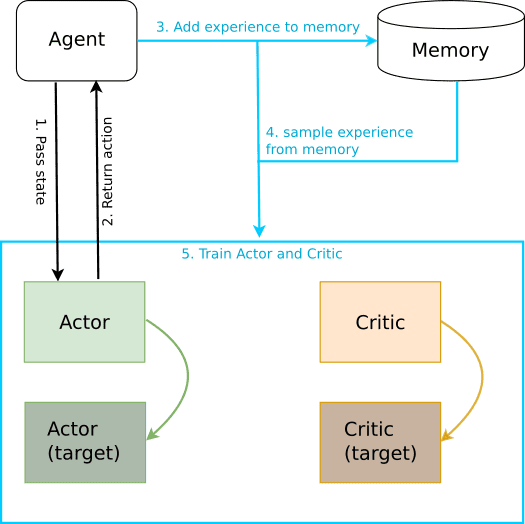
\includegraphics[width=13cm]{images_pfe/ddpgflow.png}
  \caption{Schéma représentant le processus d'entraînement de l'agent DDPG. L'agent est entraîné pour un nombre fixe d'épisodes et, dans chaque épisode, un nombre fixe de pas de temps (timesteps).}
  \label{fig:ddpg-flow}
\end{figure}
\FloatBarrier
\medskip

\begin{enumerate}
    \item \textbf{Passage de l'état à l'acteur}: L'agent reçoit un état $s_i$ de l'environnement, puis il passe cet état au réseau d'acteur ($\mu$). Le réseau d'acteur génère une action $a_i$ en fonction de l'état $s_i$. Cette action est choisie pour maximiser la valeur estimée $Q(s_i, a_i$, qui représente la somme des récompenses futures prévues.
    \item \textbf{Retour de l'action à l'agent}: L'agent reçoit l'action générée $a_i$ du réseau d'acteur, puis il l'envoie à l'environnement. Ce dernier évolue à l'étape \textit{i} et fournit une récompense et un nouvel état $s_{i+1}$ à l'agent.
    \item \textbf{Ajout des expériences à la mémoire}: L'agent crée une expérience en combinant l'état $s_i$, l'action $a_i$, la récompense et le nouvel état $s_{i+1}$ et il l'ajoute à la mémoire.
    \item \textbf{Échantillonnage des expériences de la mémoire}: l'agent échantillonne un lot (batch) d'expériences de la mémoire. Ces expériences échantillonnées forment un ensemble varié de données sur lequel l'agent va apprendre.
    \item \textbf{Entraînement de l'acteur et du critique}: L'agent utilise les expériences échantillonnées dans l'etape précédente pour mettre à jour le réseau de critique (\textit{Q}) en minimisant la différence entre les valeurs prédites et les valeurs cibles basées sur l'équation de Bellman et il calcule le gradient à partir du réseau de critique pour l'utiliser pour mettre à jour le réseau d'acteur ($\mu$). Cette mise à jour du réseau d'acteur vise à maximiser les valeurs \textit{Q} prédites.
\end{enumerate}



\section{Réglage fin après l'élagage}
A la fin de l'exécution de l'algorithme DDPG, nous aurons un modèle élagué qui va avoir une baisse de performance en raison de la perte d'informations qui peut être causée pendant l'élagage puisque nous utilisons l'élagage structuré. On ré-entraîne donc ce modèle afin d'améliorer sa précision pour atteindre une précision proche de celle du modèle original. C'est là qu'interviennent des stratégies clés telles que l'initialisation aléatoire, le rewinding, et le réglage fin (fine-tuning). Ces stratégies sont utilisées pour mettre à jour les paramètres du réseau avant l'entraînement. Dans l'initialisation aléatoire, on affecte des valeurs aléatoires aux paramètres du réseau élagué, tandis que dans le cas du rewiniding, on sauvegarde les paramètres du réseau original avant le premier entraînement pour les utiliser pour initialiser le réseau élagué. Dans le fine tuning, on initialise le réseau élagué par les valeurs des paramètres pré-élagage. La meilleure stratégie pour avoir la plus grande précision est le rewinding, mais elle ne converge pas rapidement [\cite{pfe2022}]. C'est pourquoi nous avons choisi d'utiliser le fine tuning après l'élagage car il permet d'avoir une convergence plus rapide que les deux autres stratégies [\cite{pfe2022}].

Dans cette étape, nous allons ré-entraîner le réseau élagué sur les mêmes données d'entraînement tout en maintenant les poids non supprimés fixés (nous gardons les valeurs des poids résultantes de l'élagage). Cela permet au modèle de réapprendre les relations importantes entre les caractéristiques des données et les étiquettes cibles, en se concentrant sur les parties restantes du réseau. Cependant, nous devons maintenir les poids du réseau qui ont été préservés pendant l'élagage fixés pour garantir que le réseau ne perd pas les connaissances apprises initialement.

Dans notre méthode, nous commençons le ré-entraînement avec un taux d'apprentissage plus faible que celui utilisé dans l'entraînement initial afin d'éviter des mises à jour qui pourraient perturber les poids restants.

\section{Conclusion}
Dans ce chapitre, nous avons présenté les différentes étapes suivies pour concevoir notre propre méthode automatique d'élagage. Nous avons commencé par une vue global de la méthode, où nous l'avons décomposée en quatre étapes principales: \textbf{initialisation}, \textbf{entraînement}, \textbf{élagage} et \textbf{réglage fin}. Dans la partie d'élagage, nous avons utilisé un agent DDPG qui prend en entrée un plongement d'une couche et fournit en sortie le pourcentage d'élagage de cette couche. Après l'élagage, nous avons fait un réglage fin pour améliorer la précision du modèle élagué. Nous aovns également présenté en détails la construction des plongements des couches, les métriques utilisées pour choisir les pourcentages d'élagage, le type d'élagage utilisée (élagage des couches) et l'implémentation de l'algorithme DDPG.

Dans le chapitre suivant, nous allons évaluer et tester notre méthode sur les modèles VGG-19 et ResNet-34. Nous allons présenter d'abord les technologies et outils utilisés pour la conception, puis nous allons comparer les résultats d'élagage de notre méthode avec les résultats d'élagage de quelques méthodes automatique qui effectuent le même type d'élagage que notre méthode (élagage des canaux).






\chapter{Réalisation et tests}
\section{Introduction}
Après avoir exposé en détail notre méthode automatique d'élagage dans le chapitre précèdent, nous discuterons maintenant sur les technologies et outils qui ont été choisis pour matérialiser cette approche et garantir son déploiement efficace. De ce fait, il est essentiel d'examiner en détail les langages de programmation, les bibliothèques et les frameworks qui ont été sélectionnés pour concrétiser notre approche. Nous offrons également un aperçu des stratégies de test que nous avons employées pour évaluer la performance de notre solution. Ces tests ont été établis pour mesurer les performances des modèles VGG-19 et ResNet-34 et la précision de chacun.

\section{Modèles et jeu de données utilisés}
Notre méthode d'élagage a été conçue pour élaguer les réseaux de neurones comportant seulement deux types de couches: les couches de convolution et les couches entièrement connectées. C'est pourquoi nous avons choisi d'utiliser des modèles tels que VGG-19 et ResNet-34. Dans cette section, nous parlerons de l'architecture et de l'organisation de ces deux modèles ainsi que le jeu de données CIFAR-10 qui est utilisé pour les entraîner.
\subsection{CIFAR-10}
CIFAR-10 \footnote{acronyme qui représente le "Canadian Institute for Advanced Research" (Institut canadien de recherches avancées)} est un jeu de données qui est souvent utilisé dans le domaine de la vision par ordinateur. Il se compose d'un total de 60 000 images en couleur de 32x32 pixels chacune, réparties en 10 classes différentes, avec 6 000 images par classe [\cite{krizhevsky2009learning}]. Ces 10 classes d'images comprennent: des avions, des automobiles, des oiseaux, des chats, des cerfs, des chiens, des grenouilles, des chevaux, des bateaux et des camions (\ref{fig:cifar-10-classes}).

\begin{figure}[hbt!]
  \centering
  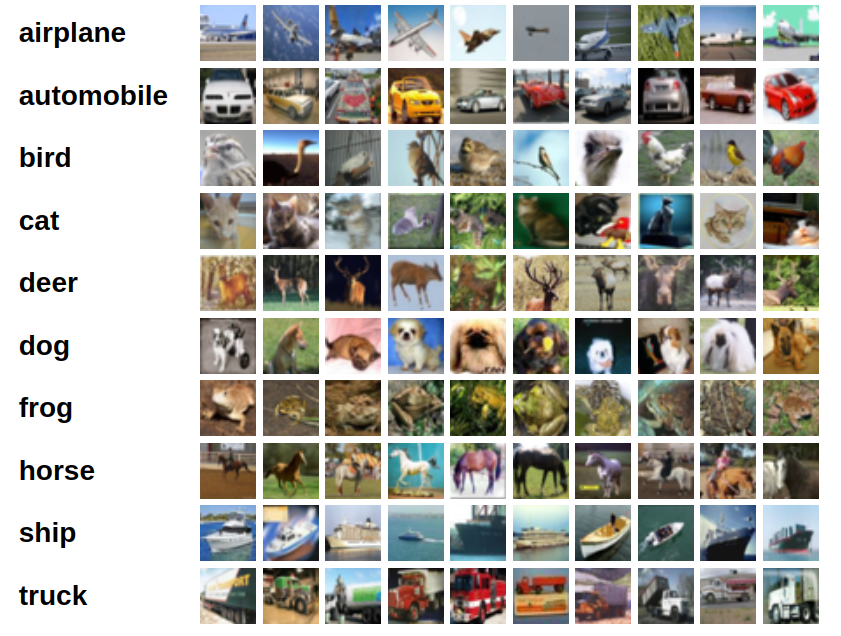
\includegraphics[width=10cm]{images_pfe/cifar-10-classes.png}
  \caption{Les classes du jeu de données CIFAR-10.}
  \label{fig:cifar-10-classes}
\end{figure}
\FloatBarrier
\medskip

Le dataset est divisé en deux ensemble: un ensemble d'entraînement et un ensemble de test. L'ensemble d'entraînement est composé de 50 000 images, tandis que l'ensemble de test est composé de 10 000 images. Dans ce dataset, les images sont de résolution relativement basse et présentent une variabilité dans les poses, l'éclairage, les arrière-plans et les détails, ce qui rend le dataset proche des défis du monde réel. Il est souvent utilisé pour l'entraînement, l'évaluation et la comparaison des performances des algorithmes de classification d'images et des réseaux de neurones convolutionnels (CNN), et il permet de reconnaître leur capacité à généraliser à partir d'un ensemble d'apprentissage limité [\cite{krizhevsky2009learning}].

\subsection{VGG-19}
VGG-19 \footnote{acronyme de "Visual Geometry Group" (famille des modèles développés par l'Université d'Oxford)} est un réseau de neurones convolutif (CNN) très profond qui possède plus de 19,6 milliards de FLOPs et est utilisé fréquemment dans le domaine de la vision par ordinateur. Il est composé de 19 couches, comprenant 16 couches de convolution et 3 couches entièrement connectées, et les images en entrée sont généralement de taille 224x224 pixels. Le réseau commence par des couches de convolutions successives, qui sont suivies de couches de pooling (de type max pooling). Ces dernières permettent de réduire la dimension spatiale de la sortie en ne conservant que les informations les plus importantes [\cite{simonyan2014very}].

Chaque couche de convolution est composée de plusieurs filtres (ou noyaux) 3x3 et un padding (stride) de 1 pour préserver les dimensions. Les filtres possèdent 64, 128, 256, 512 et 512 canaux respectivement. Le nombre de canaux augmente à mesure que l'on progresse dans le réseau. tandis que dans les couches de pooling, on a des fenêtres de 2x2 et un décalage de 2 pour réduire la résolution spatiale [\cite{simonyan2014very}]. 

Une fois que les données sont réduites en termes de dimensions spatiales, elles sont passées à travers plusieurs couches entièrement connectées afin d'effectuer la classification, en associant les caractéristiques apprises aux classes d'objets. La dernière couche de sortie possède le même nombre de neurones que de classes dans le jeu de données. Elle utilise une fonction d'activation softmax pour obtenir des probabilités normalisées pour chaque classe. Dans les couches de convolution, les fonctions d'activation utilisées sont des fonctions ReLU (Rectified Linear Unit) [\cite{simonyan2014very}].

\begin{table}[h!]
\begin{tabularx}{1.0\textwidth} { 
  | >{\centering\arraybackslash}X
  | >{\centering\arraybackslash}X 
  | >{\centering\arraybackslash}X
  | >{\centering\arraybackslash}X
  | >{\centering\arraybackslash}X
  | >{\centering\arraybackslash}X | }
 \hline
 \multicolumn{6}{|c|}{ConvNet Confguration} \\
 \hline
A & A-LRN & B & C & D & E \\
\hline
11 weight layers & 11 weight layers & 13 weight layers & 16 weight layers & 16 weight layers & 19 weight layers \\
\hline
\multicolumn{6}{|c|}{input(224 x 224 RGB image)} \\
\hline
conv 3-64 & conv 3-64 \textbf{LRN} & conv 3-64 \textbf{conv 3-64} & conv 3-64 conv 3-64 & conv 3-64 conv 3-64 & conv 3-64 conv 3-64 \\
\hline
\multicolumn{6}{|c|}{maxpool} \\
\hline
conv 3-128 & conv 3-128 & conv 3-128 \textbf{conv 3-128} & conv 3-128 conv 3-128 & conv 3-128 conv 3-128 & conv 3-128 conv 3-128 \\
\hline
\multicolumn{6}{|c|}{maxpool} \\
\hline
conv 3-256 conv 3-256 & conv 3-256 conv 3-256 & conv 3-256 conv 3-256 & conv 3-256 conv 3-256 \textbf{conv 1-256} & conv 3-256 conv 3-256 \textbf{conv 3-256} & conv 3-256 conv 3-256 conv 3-256 \textbf{conv 3-256} \\
\hline
\multicolumn{6}{|c|}{maxpool} \\
\hline
conv 3-512 conv 3-512 & conv 3-512 conv 3-512 & conv 3-512 conv 3-512 & conv 3-512 conv 3-512 \textbf{conv 1-512} & conv 3-512 conv 3-512 \textbf{conv 3-512} & conv 3-512 conv 3-512 conv 3-512 \textbf{conv 3-512} \\
\hline
\multicolumn{6}{|c|}{maxpool} \\
\hline
conv 3-512 conv 3-512 & conv 3-512 conv 3-512 & conv 3-512 conv 3-512 & conv 3-512 conv 3-512 \textbf{conv 1-512} & conv 3-512 conv 3-512 \textbf{conv 3-512} & conv 3-512 conv 3-512 conv 3-512 \textbf{conv 3-512} \\
\hline
\multicolumn{6}{|c|}{maxpool} \\
\hline
\multicolumn{6}{|c|}{FC-4096} \\
\hline
\multicolumn{6}{|c|}{FC-4096} \\
\hline
\multicolumn{6}{|c|}{FC-1000} \\
\hline
\multicolumn{6}{|c|}{soft-max} \\
\hline
\end{tabularx}
\caption{Les configurations des réseaux VGG (illustrées dans des colonnes selon leurs profondeurs). La colonne E représente la configuration du modèle VGG-19 utilisé [\cite{simonyan2014very}].}
\label{table:vgg-configurations}
\end{table}

\subsection{ResNet-34}
ResNet-34 est un réseau de neurones résiduel profond, composé de 34 couches et possédant plus de 3,6 milliards de FLOPs. Ce type de réseau est caractérisé par l'utilisation de blocs résiduels, en introduisant des connexions résiduelles, également appelées connexions "skip", qui sautent une ou plusieurs couches. Cette caractéristique permet d'exploiter les avantages de la profondeur tout en évitant les problèmes de dégradation de performance qui surviennent lorsque les réseaux deviennent plus profonds [\cite{He_2016_CVPR}].

Le bloc résiduel de base dans ResNet-34 comprend deux couches de convolution 3x3 accompagnées de fonctions d'activation ReLU, et intègre une connexion résiduelle qui agit comme un raccourci autour des couches de convolution, en ajoutant la sortie de la première couche de convolution à la sortie de la deuxième couche. 

\begin{figure}[hbt!]
  \centering
  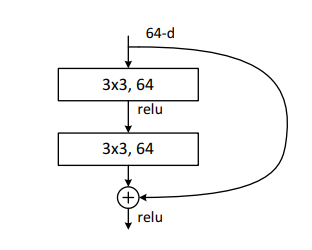
\includegraphics[width=10cm]{images_pfe/residual-bloc.png}
  \caption{Un bloc résiduel de base comme sur la figure \ref{fig:architectures} pour ResNet-34 [\cite{He_2016_CVPR}].}
  \label{fig:residual-bloc}
\end{figure}
\FloatBarrier
\medskip

La fin du réseau ResNet-34 comprend une couche de classification entièrement connectée avec autant de neurones que de classes dans le jeu de données. Une fonction d'activation softmax est généralement utilisée pour obtenir les probabilités de classe normalisées.

\begin{figure}[hbt!]
  \centering
  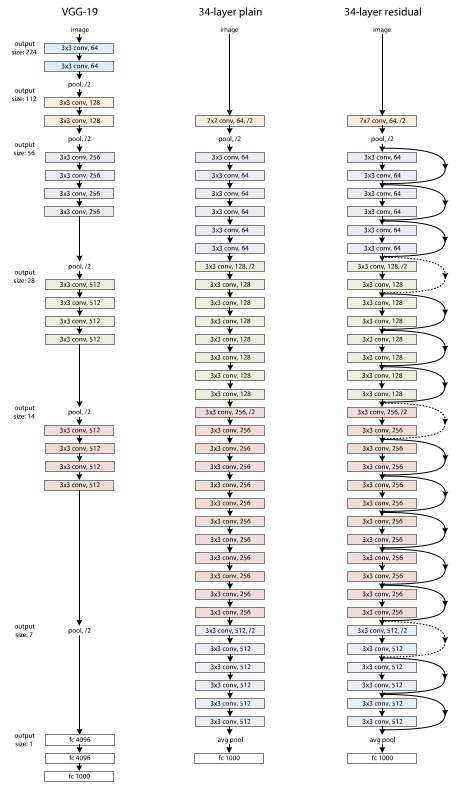
\includegraphics[width=13.5cm]{images_pfe/vgg-19-and-resnet-34.png}
  \caption{Les architectures des modèles utilisés. A gauche: le modèle VGG-19. Au milieu: un réseau simple de 34 couches. À droite: le modèle ResNet-34 [\cite{He_2016_CVPR}].}
  \label{fig:architectures}
\end{figure}
\FloatBarrier
\medskip

\section{Technologies utilisées}
\subsection{Python}

\begin{figure}[hbt!]
  \centering
  
\includegraphics[width=4cm]{images_pfe/python.png}
  \caption{Python.}
  \label{fig:python}
\end{figure}
\FloatBarrier
\medskip

Python joue un rôle important dans le domaine de l'intelligence artificielle (IA) grâce à sa polyvalence, sa simplicité et sa richesse en bibliothèques spécialisées. En tant que langage de programmation, Python est devenu le premier choix  pour de nombreux chercheurs, ingénieurs et développeurs travaillant dans le domaine de l'IA. D'une part, Python est connu pour sa syntaxe claire et lisible, ce qui  permet aux nouveaux arrivants dans le domaine de l'IA de se familiariser rapidement avec les concepts de base. D'autre part, Python offre plusieurs bibliothèques et frameworks spécialisés dans l'IA, tels que TensorFlow, Keras, PyTorch et Scikit-learn. Ces bibliothèques sont souvent utilisées pour le développement de réseaux de neurones, d'algorithmes d'apprentissage automatique et d'autres techniques d'IA. Finalement, Python est un langage polyvalent qui permet aux développeurs de créer et tester différentes approches rapidement.

\section{Bibliothèque utilisées}
Python offre une riche collection de bibliothèques spécialisées dans plusieurs domaines, en particulier l'IA. Ces bibliothèques offrent des outils et des frameworks puissants pour développer des modèles d'apprentissage automatique, des réseaux de neurones, et bien plus encore. Dans cette section, nous allons explorer les bibliothèques que nous avons utilisé pour implémenter et tester notre méthode.
\subsection{NumPy}

\begin{figure}[hbt!]
  \centering
  
\includegraphics[width=4cm]{images_pfe/numpy.png}
  \caption{NumPy.}
  \label{fig:numpy}
\end{figure}
\FloatBarrier
\medskip

NumPy \footnote{acronyme de "Numerical Python"} est une bibliothèque open source qui offre de nombreuses fonctionnalités pour le calcul numérique en Python. Elle offre un support puissant pour la manipulation de tableaux multidimensionnels, ainsi que pour l'exécution de calculs mathématiques complexes sur ces tableaux. Ces tableaux multidimensionnels permettent de stocker et de manipuler efficacement des données numériques sous forme de matrices et de vecteurs. Elle fournit également des fonctions mathématiques de base, des opérations d'algèbre linéaire, des opérations sur les tableaux, des fonctions statistiques et bien plus encore. Elle est largement utilisé en IA pour le traitement et la manipulation de données, la préparation de jeux de données, ainsi que pour la mise en œuvre d'algorithmes d'apprentissage automatique et de réseaux de neurones. La performance élevée de NumPy en calcul numérique en fait un bon choix pour les tâches intensives en termes de calcul.


\subsection{Matplotlib}
\begin{figure}[hbt!]
  \centering
  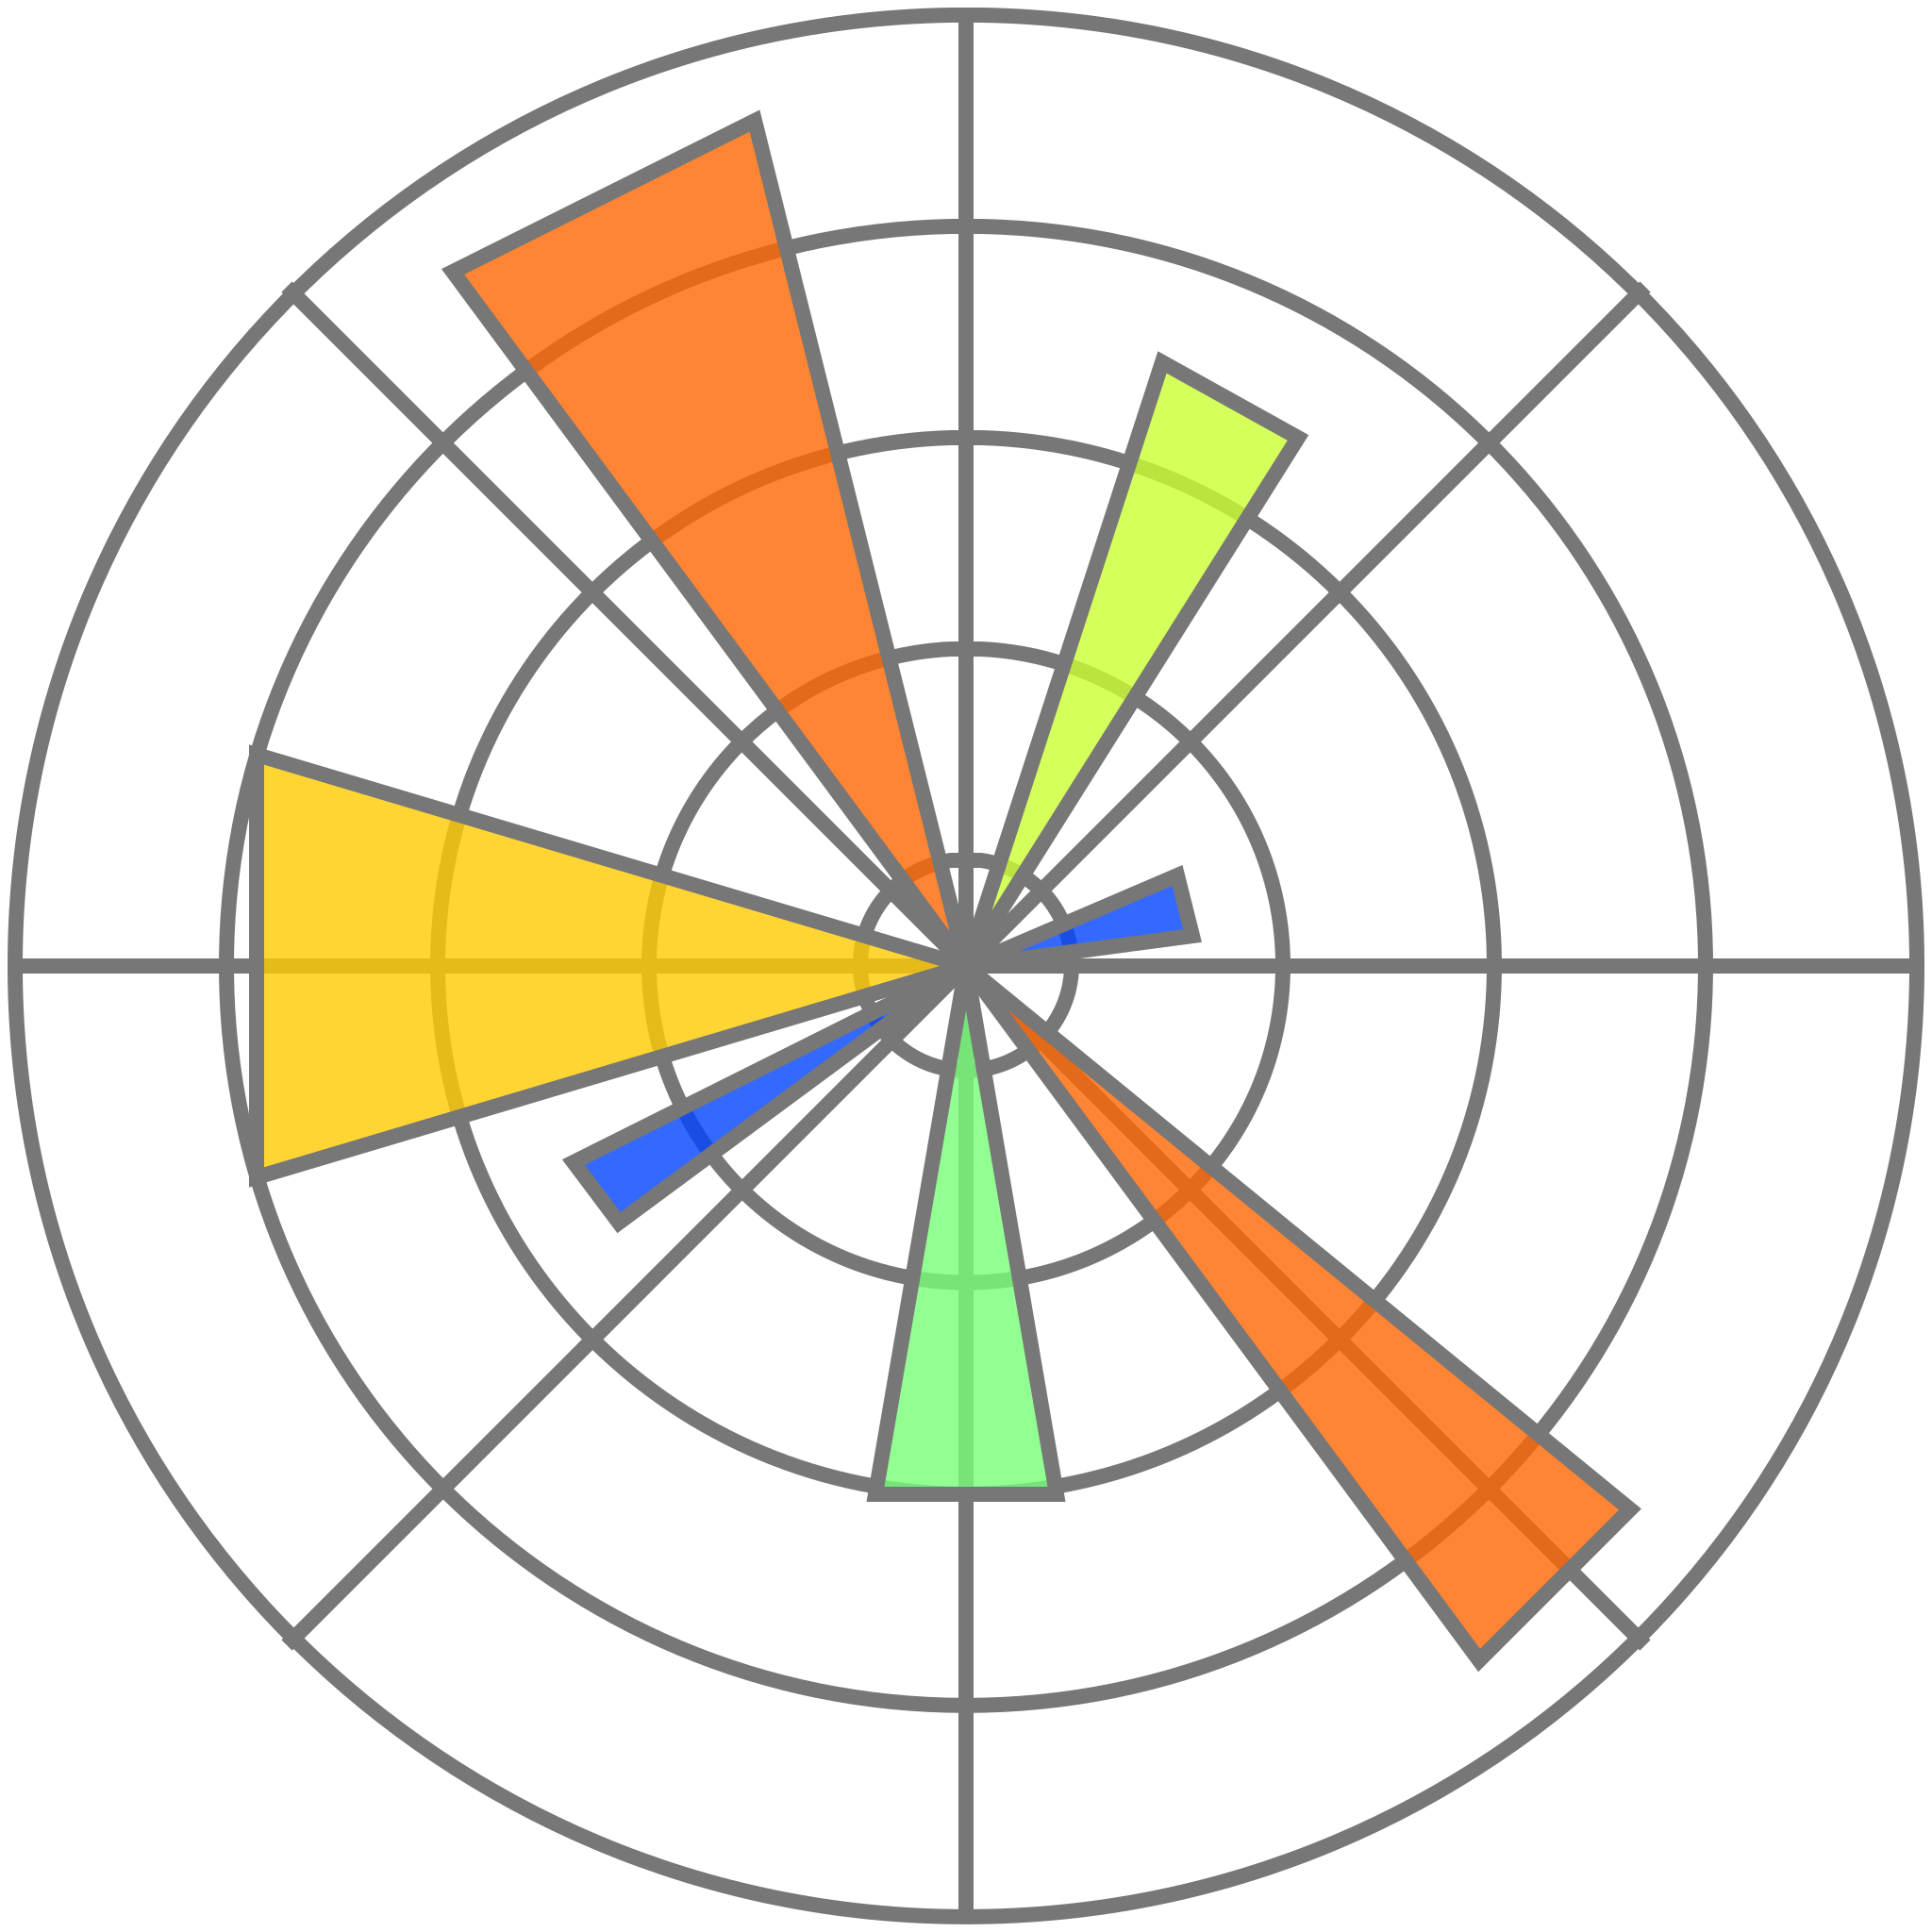
\includegraphics[width=4.5cm]{images_pfe/matplotlib.png}
  \caption{Matplotlib.}
  \label{fig:matplotlib}
\end{figure}
\FloatBarrier
\medskip

Matplotlib est une bibliothèque de visualisation en Python qui aide à créer des graphiques et des visualisations de données de manière interactive et statique. Cette bibliothèque offre un large éventail d'outils pour générer des graphiques de haute qualité à partir de données numériques. Son objectif est de permettre aux utilisateurs de représenter visuellement des données complexes de manière claire et compréhensible. Pour cela, elle propose une grande variété de types de graphiques, tels que les graphiques linéaires, les graphiques en barres, les graphiques à secteurs, les graphiques de dispersion, les graphiques 3D, etc. Elle permet également de personnaliser presque tous les aspects des graphiques, y compris les étiquettes, les couleurs, les styles de ligne, les titres, les axes et les légendes. L'utilisation de Matplotlib est essentielle dans l'analyse de données, la science des données et la recherche en général. En intelligence artificielle et en apprentissage automatique, Matplotlib est souvent employé pour visualiser les performances des modèles, les distributions de données, les tendances, les caractéristiques importantes, les matrices de confusion, les courbes d'apprentissage, etc.

\subsection{Pytorch}

\begin{figure}[hbt!]
  \centering
  
\includegraphics[width=4cm]{images_pfe/pytorch.png}
  \caption{Pytorch.}
  \label{fig:pytorch}
\end{figure}
\FloatBarrier
\medskip

PyTorch est une bibliothèque open-source d'apprentissage automatique et d'intelligence artificielle en Python, développée principalement par Facebook's AI Research lab (FAIR). Elle repose sur un concept fondamental appelé "tenseur", qui est une structure de données multidimensionnelle similaire aux tableaux NumPy et elle est conçue pour faciliter le développement et la mise en œuvre de modèles de réseaux de neurones profonds. PyTorch est surtout distinguée par sa prise en charge des calculs automatiques de gradients, ce qui signifie qu'il est possible de définir des opérations mathématiques sur les tenseurs et que PyTorch peut automatiquement calculer les gradients de ces opérations qui sont nécessaires pour ajuster les poids dans les réseaux de neurones et ainsi minimiser une fonction de perte. Elle est utilisé pour la conception des modèles de réseaux de neurones profonds, y compris les réseaux de neurones convolutionnels (CNN), les réseaux de neurones récurrents (RNN), les transformeurs, etc.

\subsection{Torchvision}

\begin{figure}[hbt!]
  \centering
  
\includegraphics[width=4cm]{images_pfe/torchvision.png}
  \caption{Torchvision.}
  \label{fig:torchvision}
\end{figure}
\FloatBarrier
\medskip

Torchvision est une bibliothèque qui fait partie de PyTorch. Elle est spécifiquement conçue pour faciliter le chargement et la transformation de jeux de données d'images couramment utilisés dans le domaine de l'apprentissage automatique et de la vision par ordinateur. Elle offre des outils pour prétraiter les données d'image, créer des ensembles de données, appliquer des transformations aux images et charger des ensembles de données préexistants. Elle propose des classes pour charger facilement des ensembles de données standard tels que MNIST, CIFAR-10, ImageNet, etc. Elle permet également d'appliquer diverses transformations aux images, telles que le redimensionnement, le recadrage, la normalisation, les rotations, les miroirs, etc. qui sont utiles pour augmenter la variabilité des données.

\subsection{NNI}

\begin{figure}[hbt!]
  \centering
  
\includegraphics[width=6cm]{images_pfe/nni.png}
  \caption{NNI (Neural Network Intelligence).}
  \label{fig:nni}
\end{figure}
\FloatBarrier
\medskip

NNI (Neural Network Intelligence) est une bibliothèque open-source développée par Microsoft Research. Elle fournit un ensemble d'outils et de bibliothèques pour faciliter l'exploration et l'optimisation des espaces d'hyperparamètres, ainsi que pour la recherche automatique d'architectures de modèles. Elle permet aux utilisateurs de définir un espace de recherche pour les hyperparamètres, tels que les taux d'apprentissage, les tailles de lot, les architectures de couches, etc. NNI exécute ensuite des expériences en utilisant différentes configurations d'hyperparamètres et rapporte les résultats, y compris les performances du modèle. Elle est très utile dans le domaine de l'apprentissage automatique, car elle simplifie et automatise le processus d'ajustement des hyperparamètres et d'exploration des architectures, ce qui peut considérablement accélérer le développement de modèles performants.

\section{Outils utilisés}

\subsection{Google Colab}

\begin{figure}[hbt!]
  \centering
  \includegraphics[width=7cm]{images_pfe/colab.png}
  \caption{Google Colab.}
  \label{fig:colab}
\end{figure}
\FloatBarrier
\medskip

Google Colab (abrégé de Colaboratory) est une plateforme de notebooks interactifs basée sur le cloud, développée par Google. Elle permet aux utilisateurs d'écrire, d'exécuter et de partager du code Python de manière collaborative, sans nécessiter de configuration ou d'installation. Elle propose des notebooks interactifs qui permettent d'insérer des cellules de code exécutable et des cellules de texte et chaque notebook Colab s'exécute dans un environnement virtuel où les utilisateurs peuvent accéder à la puissance de calcul des processeurs graphiques (GPU) et des unités de traitement tensoriel (TPU) pour accélérer l'entraînement de modèles d'apprentissage automatique. Elle propose également de nombreuses bibliothèques préinstallées, mais les utilisateurs peuvent également installer et utiliser des bibliothèques tierces via des commandes simples.

\subsection{Google Drive}

\begin{figure}[hbt!]
  \centering
  \includegraphics[width=6cm]{images_pfe/drive.png}
  \caption{Google Drive.}
  \label{fig:drive}
\end{figure}
\FloatBarrier
\medskip

Google Drive est un service de stockage en ligne développé par Google pour stocker, synchroniser et partager des fichiers et des dossiers sur le cloud. Il offre une variété de fonctionnalités telles que le stockage en ligne, la synchronisation multi-appareils, le partage de fichiers, la collaboration en temps réel, etc. De plus, il peut être utilisé avec Google Colab.

\section{Tests et résultats}
Cette dernière section présente une analyse des résultats obtenus après avoir tester notre méthode d'élagage. Nous effectuons nos expérimentations sur CIFAR-10 avec deux réseaux profonds classiques: VGG-19 et ResNet-34. Les résultats obtenus sont examinés et comparés avec les résultats des autres méthodes d'élagage, permettant ainsi de dégager des conclusions quant à la performance et l'efficacité de notre méthode. Cette section donc vise à présenter de manière claire et précise les découvertes issues de ces tests.

Le processus d'exécution des tests est décrit comme suit:
\begin{enumerate}
    \item Entraînement du modèle jusqu'à la convergence
    \item Élagage du modèle avec les pourcentages d'élagage fournis par l'agent DDPG
    \item Réglage fin du modèle
    \item Mesure de la précision, la taille, le nombre de paramètres, etc. du modèle élagué
    \item Comparaison du modèle élagué avec le modèle original
\end{enumerate}

On élague les canaux dont les poids ont la plus petite valeur absolue. Le pourcentage d'élagage maximum $a_{max}$ est fixé pour les couches de convolution à 0,8 et pour la couche entièrement connectée à 0,98. Cette limite supérieure $a_{max}$ est utilisée uniquement pour accélérer la recherche. Nous pouvons simplement prendre $a_{max} = 1$ et nous aurons des résultats similaires. Le réseau d’acteurs $\mu$ comporte deux couches cachées, chacune comportant 300 neurones et la couche de sortie finale est une couche sigmoïde pour délimiter les actions dans la plage (0, 1). Le réseau critique \textit{Q} comportait également deux couches cachées, chacune comptant 300 unités. Nous entraînons le réseau avec 64 comme batch size. L'agent DDPG explore d’abord 100 épisodes avec un bruit constant $\sigma = 0.5$, puis exploite 300 épisodes avec un bruit $\sigma$ qui décroît de manière exponentielle.

Pour évaluer la performance de notre méthode, nous l'avons comparée avec les deux méthodes d'élagage citées dans la première partie du rapport: ABCPruner [\cite{lin2020channel}] et CCPrune [\cite{CHEN202135}]. Ces deux méthodes sont des méthodes automatique qui utilisent le même type d'élagage (élagage des canaux). ABCPruner est une méthode basée sur l'algorithme de colonie d'abeilles artificielles (ABC). Dans cette méthode, la recherche du réseau élagué optimal est formulée comme un problème d'optimisation et l'algorithme ABC est utilisé pour le résoudre de manière automatique afin de réduire les interférences humaines. CCPrune (Collaborative Channel Pruning) est une autre méthode qui utilise aussi l'élagage des canaux. Cette méthode introduit d’abord la régularisation sur les poids des couches de convolution et les facteurs d’échelle de la couche BN (Batch Normalization) respectivement, puis elle combine les poids de la couche de convolution et le facteur d’échelle de la couche BN pour évaluer l’importance du canal.

\clearpage

\subsection{VGG-19}
Le tableau suivant représente les résultats après l'application de notre méthode sur VGG-19 avec une comparaison aux deux autres méthodes d'élagage: ABCPruner et CCPrune.

\begin{table}[h!]
\begin{tabular}{|p{3.25cm}|p{3cm}|p{2.25cm}|p{3cm}|p{2.25cm}|}
\hline
Méthode & Précision (\%) & FLOPs (\%) & Paramètres (\%) & Taille (MB) \\
\hline
Modèle original & 93.71 & - & - & 548 \\
\hline
ABCPruner & 93.08 & 73.68 & 88.68 & 62.6 \\
\hline
CCPrune & \textbf{93.78} & 48.92 & 86.82 & 77.2 \\
\hline
Notre méthode & 90.6 & 91.6 & 90.2 & \textbf{52.7} \\
\hline
\end{tabular}
\caption{Résultats d'élagage de VGG-19 sur CIFAR-10. La deuxième colonne indique la précision du modèle. Les troisième et quatrième colonnes indiquent le taux d'élagage des FLOPs et le taux d'élagage des paramètres. La dernière colonne indique la taille du modèle.}
\label{table:vgg-pruning-results}
\end{table}

Les résultats dans le tableau \ref{table:vgg-pruning-results} montrent que les techniques ABCPruner et CCPrune atteignent toujours une précision très proche du réseau original qui est aussi meilleure que celle de notre méthode. Cependant, notre méthode dépasse ces techniques quand nous parlons de la taille du modèle. Nous remarquons qu'avec notre méthode, nous pouvons d'avoir une grande réduction dans la taille du modèle (la taille est 10 fois moins que le modèle original) et dans le nombre de FLOPs et paramètres à cause des pourcentages d'élagage élevés. Cette réduction du nombre de FLOPs signifie que notre méthode effectue moins de calculs que les deux autres méthodes. Nous pouvons donc avoir le meilleur temps d'inférence avec notre méthode. Nous pouvons aussi remarquer que l'utilisation de l'élagage structuré engendre une petite dégradation de la précision des modèles élagués par rapport au modèle original. Cette dégradation est causée par la suppression de canaux entiers, ce qui peut causer une suppression de certains paramètres importants qui peuvent se trouver dans l'un des canaux éliminées.

La figure \ref{fig:vgg-channels} montre les statistiques des canaux restants dans les couche de convolution dans le modèle VGG-19. Sur cette figure, Nous pouvons clairement comprendre la structure du réseau après l'élagage.

Dans VGG-19, 90\% des poids sont dans les couches entièrement connectées. Dans notre méthode, nous avons utilisé l’élagage de canaux entiers en couches de convolution et cela a un effet secondaire intéressant en réduisant également la mémoire. Comme observé dans \cite{molchanov2016pruning}, plus la couche est profonde, plus elle sera élaguée. Cela signifie que la dernière couche de convolution sera beaucoup élaguée et que de nombreux neurones de la couche entièrement connectée qui la suit seront également supprimés.

\begin{figure}[hbt!]
  \centering
  \includegraphics[width=14cm]{images_pfe/vgg-channels.png}
  \caption{Statistiques des canaux restants dans les couches de convolution de VGG-19.}
  \label{fig:vgg-channels}
\end{figure}
\FloatBarrier
\medskip

\subsection{ResNet-34}
Le tableau suivant représente les résultats après l'application de notre méthode sur ResNet-34 et une comparaison avec les deux autres méthodes d'élagage utilisées: ABCPruner et CCPrune.

\begin{table}[h!]
\begin{tabular}{|p{3.25cm}|p{3cm}|p{2.25cm}|p{3cm}|p{2.25cm}|}
\hline
Méthode & Précision (\%) & FLOPs (\%) & Paramètres (\%) & Taille (MB) \\
\hline
Modèle original & 91.45 & - & - & 81.4 \\
\hline
ABCPruner & 89.69 & 58.97 & 51.76 & 39.2 \\
\hline
CCPrune & \textbf{90.76} & 57.55 & 34.78 & 53.0 \\
\hline
Notre méthode & 86.21 & 58.09 & 67.63 & \textbf{26.5} \\
\hline
\end{tabular}
\caption{Résultats d'élagage de ResNet-34 sur CIFAR-10. La deuxième colonne indique la précision du modèle. Les troisième et quatrième colonnes indiquent le taux d'élagage des FLOPs et le taux d'élagage des paramètres. La dernière colonne indique la taille du modèle.}
\label{table:resnet-pruning-results}
\end{table}

Les résultats dans le tableau \ref{table:resnet-pruning-results} sont les même que ceux du modèle
VGG-19. Ils montrent toujours que la précision dans les techniques ABCPruner et CCPrune dépasse la précision dans notre méthode. Cependant, notre méthode dépasse ces deux techniques dans la compression de la taille du modèle et dans le nombre de FLOPs, ce qui nous donnera un meilleur temps d'inférence. Nous remarquons aussi que la taille du modèle élagué avec notre méthode est presque 3 fois moins que le modèle original, ainsi que le nombre de FLOPs et paramètres (les résultats sont résumés dans la figure \ref{fig:resnet-pruning}). Nous avons aussi vu que l'élagage structuré réduit légèrement la précision des modèles élagués par rapport au modèle original et la cause de cette réduction est la même cause mentionnée dans l’interprétation de l’élagage structuré pour le modèle VGG-19.

\begin{figure}[hbt!]
  \centering
  \includegraphics[width=14cm]{images_pfe/resnet-pruning.png}
  \caption{Comparaison entre les taux d'élagage des FLOPs et des paramètres des trois méthodes d'élagage pour le réseau ResNet-34.}
  \label{fig:resnet-pruning}
\end{figure}
\FloatBarrier
\medskip

\section{Conclusion}
En conclusion de ce chapitre dédié aux tests et résultats, l'analyse des résultats d'expérimentations menées sur les modèles VGG-19 et ResNet-34 prouvent l'efficacité de notre méthode d'élagage automatique. Nous avons trouvé que notre méthode permet de réduire significativement la taille des modèles et le nombre de FLOPs, en surpassant les deux méthodes utilisées pour la comparaison (ABCPruner et CCPrune). Ces réductions nous permettent d'avoir de très petits modèles qui sont également très performants et faciles à déployer sur des appareils limités en termes de ressources de calcul et de stockage. Cependant, il est important de souligner que le processus d'élagage n'est pas sans compromis. Les avantages en termes de taille sont parfois accompagnés d'une petite dégradation de la précision qui nécessite de faire un réglage fin après l'élagage afin de restaurer partiellement les performances du modèle initial. De plus, le taux d'élagage optimal peut varier en fonction du même jeu de données et des spécificités de la tâche.

On a également présentée au début du chapitre les modèles utilises pour tester la méthode (VGG-19 et ResNet-34) et le jeu de données utilisé (CIFAR-10) pour l'entraînement de ces modèles, ainsi que les différents technologies et outils utilisés pour la conception de notre méthode. Nous avons utilisé le langage de programmation Python avec plusieurs bibliothèques telles que NumPy, Matplotlib, Pytorch, etc. Ces bibliothèques offrent des outils puissants pour développer et entraîner les différents types de réseaux de neurones.

Enfin, ce chapitre constitue une étape essentielle de ce rapport en fournissant des résultats d'implémentation des concepts et des théories énoncés dans le chapitre précédent. Les résultats obtenus offrent des orientations pratiques pour les applications et les améliorations futures de cette méthode pour élaguer des réseaux de neurones profonds. En considérant ces résultats, la rapport se tourne vers la section finale, où les conclusions et perspectives globales sont tirées.

\chapter*{Conclusion et perspectives}
\addcontentsline{toc}{chapter}{Conclusion et perspectives}
\markboth{Conclusion et perspectives}{Conclusion et perspectives}
\label{chap:conclusion}
%\minitoc

Avec l'augmentation de la profondeur des architecture des réseaux de neurones, le nombre de calculs et la taille des réseaux augmentent également, ce qui rend leurs déploiement sur des appareils dotés d'un matériel limité très difficile et compliqué. L'élagage a émergé comme une approche pour réduire la complexité de ces réseaux profonds. Cependant, cette approche prend beaucoup de temps et nécessite des experts humains afin de bien élaguer un réseau. En raison de ses défauts, des méthodes automatiques utilisant l'apprentissage par renforcement sont apparues. Ces méthodes fournissent des résultats exceptionnels et ont la capacité à s'adapter à une grande variété d'environnements en utilisant des configurations appropriées. Cependant, les algorithmes d'apprentissage par renforcement ne peuvent pas prendre en entrée un réseau profond complet car il est très complexe. Il est donc nécessaire d'utiliser des structures moins complexes comme entrée telles que le plongement de graphe, de chouche, de noeuds, etc. Le plongement est un vecteur unidimentionnel qui garde seulement les informations importantes dans le réseau. En transformant ces données en un vecteur unidimensionnel, cet outil de plongement facilite grandement la capacité de l'agent d'apprentissage par renforcement à appréhender et à interagir avec son environnement.

Dans ce rapport, nous avons découvert les différentes techniques d'élagage des réseaux de neurones, ainsi que les types de plongements et les différents aspects des algorithmes d'apprentissage par renforcement. Nous avons commencé le rapport par une introduction au domaine d'apprentissage profond où nous avons vu quelques définitions et concepts de base, tels que les poids, les connexions, les types de réseaux de neurones, les différents types d'apprentissage (supervisé, non-supervisé, semi-supervisé et par renforcement), etc. Ensuite, nous avons présenté quelques concepts et algorithmes de l'apprentissage par renforcement, tels que les processus de décision de Markov, l'apprentissage Q profond, etc. Nous avons également parlée sur les graphes et les différentes techniques de plongement, ainsi que l'hypothèse du ticket de loterie et les types d'élagage des réseaux de neurones.

On a parlé de tout cela juste pour acquérir suffisamment de connaissances pour pouvoir élaborer une nouvelle approche d'élagage des réseaux de neurones profonds, en utilisant les techniques de plongement de couches et un algorithme d'apprentissage par renforcement complexe pour nous fournir les pourcentage d'élagage du modèle, pour arriver enfin à un modèle de taille considérablement réduite et avec une réduction minimale de la précision. Nous avons commencé par la présentation des modèles testés et le jeux de données utilisée pour les entraîner. Puis, nous avons présenté une vue global de la solution et ensuite les détails de chaque étape de la solution, qui commence par la construction du plongement et finit par le réglage fin. Enfin, nous avons vu les différents résultats d'application de notre méthode sur les modèles et nous les avons comparés avec les résultats de quelques méthodes performantes.

L'avantage le plus important de notre méthode est qu'elle permet de réduire considérablement la taille des modèles et le nombre de calculs, ce qui est idéal pour déployer ces modèles sur des appareils dotés d'un matériel limité. Toutefois, cet avantage est parfois accompagné d'une petite dégradation de la précision, ce qui nécessite de faire un réglage fin après l'élagage afin de restaurer partiellement la précision du modèle initial.

Même si notre méthode donne de très bons résultats, des améliorations sont encore possibles. Nous pouvons apporter ces améliorations à différentes parties de notre processus d’élagage. Par exemple, nous pouvons essayer de généraliser notre méthode à d'autres types d’architectures de réseau autres que les réseaux convolutifs et résiduels. Nous pouvons également modifier l'algorithme d'élagage de l'élagage des canaux vers un autre type d'élagage qui peut contribuer à augmenter la précision de nos modèles. Nous pouvons également essayer de faire d'autres types de plongement, tels que le plongement de l'ensemble du réseau, et utiliser d'autres algorithmes d'apprentissage par renforcement, tels que PPO ou A3C, ou même essayer un algorithme d'optimisation. Nous pouvons aussi essayer de faire l'élagage au début ou pendant l'entraînement afin d'éviter l'étape de réglage fin qui peut prendre du temps pour le ré-entraînement.
\chapter{Réalisation}

\newpage

\section{Introduction}
Lorem ipsum dolor sit amet, consectetur adipiscing elit. Proin posuere euismod neque, non semper nibh viverra sed. Praesent ut varius magna. Fusce ipsum ante, semper nec interdum at, semper et lacus. Nulla ultrices magna a fringilla finibus. Etiam sollicitudin blandit ante. Vivamus blandit rhoncus tincidunt. Morbi sit amet congue purus. Praesent interdum gravida congue. Donec fermentum dui fermentum maximus rutrum.

\section{Architecture technique de la solution}

\begin{figure}[hbt!]
  \centering
  \includegraphics[height=15cm]{images_pfe/SYSTEM_ARCHITECTURE.png}
  \caption{Architecture technique de la solution.}
  \label{fig:technical-architecture}
\end{figure}
\FloatBarrier

La figure \ref{fig:technical-architecture} Lorem ipsum dolor sit amet, consectetur adipiscing elit. Proin posuere euismod neque, non semper nibh viverra sed. Praesent ut varius magna.Lorem ipsum dolor sit amet, consectetur adipiscing elit. Proin posuere euismod neque, non semper nibh viverra sed. Praesent ut varius magna. \textbf{Teradata Database} et il Lorem ipsum dolor sit amet, consectetur adipiscing elit. Proin posuere euismod neque, non semper nibh viverra sed. Praesent ut varius magna. \textbf{Apache Nifi} Lorem ipsum dolor sit amet, consectetur adipiscing elit. Proin posuere euismod neque, non semper nibh viverra sed. Praesent ut varius magna. \textbf{Apache Spark} via l'API Python \textbf{PySpark}. Lorem ipsum dolor sit amet, consectetur adipiscing elit. Proin posuere euismod neque, non semper nibh viverra sed. Praesent ut varius magna. \textbf{PostgreSQL} Lorem ipsum dolor sit amet, consectetur adipiscing elit. Proin posuere euismod neque, non semper nibh viverra sed. Praesent ut varius magna. \textbf{Django} sous le langage \textbf{Python}. Lorem ipsum dolor sit amet, consectetur adipiscing elit. Proin posuere euismod neque, non semper nibh viverra sed. Praesent ut varius magna. \textbf{Django Rest}. Le client web quant à lui, est implémenté avec la librairie \textbf{React.js} sous le langage \textbf{Javascript}. Le système communique avec les APIs \textbf{Google Maps} Lorem ipsum dolor sit amet, consectetur adipiscing elit. Proin posuere euismod neque, non semper nibh viverra sed. Praesent ut varius magna.I \textbf{Distance Matrix} Lorem ipsum dolor sit amet, consectetur adipiscing elit. Proin posuere euismod neque, non semper nibh viverra sed. Praesent ut varius magna. \textbf{Directions} Lorem ipsum dolor sit amet, consectetur adipiscing elit. Proin posuere euismod neque, non semper nibh viverra sed. Praesent ut varius magna.\textbf{Maps} Lorem ipsum dolor sit amet, consectetur adipiscing elit. Proin posuere euismod neque, non semper nibh viverra sed. Praesent ut varius magna.

\section{Technologies utilisées}

\subsection*{Teradata Database}

\begin{wrapfigure}{r}{0.3\textwidth}
  \centering
  \includegraphics[width=0.28\textwidth]{images_pfe/Teradata_logo_2018.png}
  \caption{Logo de Teradata.}
\end{wrapfigure}
\FloatBarrier
Teradata Database \footnote{\url{https://www.teradata.com/} (visité le 11/08/2020).} Lorem ipsum dolor sit amet, consectetur adipiscing elit. Proin posuere euismod neque, non semper nibh viverra sed. Praesent ut varius magna. Fusce ipsum ante, semper nec interdum at, semper et lacus. Nulla ultrices magna a fringilla finibus. Etiam sollicitudin blandit ante. Vivamus blandit rhoncus tincidunt. Morbi sit amet congue purus. Praesent interdum gravida congue. Donec fermentum dui fermentum maximus rutrum.

\subsection*{Apache Nifi}
\begin{wrapfigure}{r}{0.3\textwidth}
  \centering
  \includegraphics[width=0.2\textwidth]{images_pfe/apache_nifi_logo.png}
  \caption{Logo de Nifi.}
\end{wrapfigure}
\FloatBarrier
Apache Nifi \footnote{\url{https://nifi.apache.org/} (visité le 11/08/2020).} Lorem ipsum dolor sit amet, consectetur adipiscing elit. Proin posuere euismod neque, non semper nibh viverra sed. Praesent ut varius magna. Fusce ipsum ante, semper nec interdum at, semper et lacus. Nulla ultrices magna a fringilla finibus. Etiam sollicitudin blandit ante. Vivamus blandit rhoncus tincidunt. Morbi sit amet congue purus. Praesent interdum gravida congue. Donec fermentum dui fermentum maximus rutrum.


\subsection*{Apache Spark}
\begin{wrapfigure}{r}{0.3\textwidth}
  \centering
  \includegraphics[width=0.28\textwidth]{images_pfe/Apache_Spark_logo.png}
  \caption{Logo de Spark.}
\end{wrapfigure}
\FloatBarrier
Apache Spark \footnote{\url{https://spark.apache.org/} (visité le 11/08/2020).} Lorem ipsum dolor sit amet, consectetur adipiscing elit. Proin posuere euismod neque, non semper nibh viverra sed. Praesent ut varius magna. (\textbf{PySpark}) Lorem ipsum dolor sit amet, consectetur adipiscing elit. Proin posuere euismod neque, non semper nibh viverra sed. Praesent ut varius magna. Fusce ipsum ante, semper nec interdum at, semper et lacus. Nulla ultrices magna a fringilla finibus. Etiam sollicitudin blandit ante. Vivamus blandit rhoncus tincidunt. Morbi sit amet congue purus. Praesent interdum gravida congue. Donec fermentum dui fermentum maximus rutrum.


\subsection*{PostgreSQL}
\begin{wrapfigure}[9]{r}{0.3\textwidth}
  \centering
  \includegraphics[width=0.2\textwidth]{images_pfe/postgres_logo.png}
  \caption{Logo de PostgreSQL.}
\end{wrapfigure}
\FloatBarrier
PostgreSQL \footnote{\url{https://www.postgresql.org/} (visité le 11/08/2020).} Lorem ipsum dolor sit amet, consectetur adipiscing elit. Proin posuere euismod neque, non semper nibh viverra sed. Praesent ut varius magna. Fusce ipsum ante, semper nec interdum at, semper et lacus. Nulla ultrices magna a fringilla finibus. Etiam sollicitudin blandit ante. Vivamus blandit rhoncus tincidunt. Morbi sit amet congue purus. Praesent interdum gravida congue. Donec fermentum dui fermentum maximus rutrum.


\subsection*{Python}

\begin{wrapfigure}[6]{r}{0.3\textwidth}
  \centering
  \includegraphics[width=0.12\textwidth]{images_pfe/python_logo.png}
  \caption{Logo de Python.}
\end{wrapfigure}
\FloatBarrier
Python \footnote{\url{https://www.python.org/} (visité le 11/08/2020).} Lorem ipsum dolor sit amet, consectetur adipiscing elit. Proin posuere euismod neque, non semper nibh viverra sed. Praesent ut varius magna. Fusce ipsum ante, semper nec interdum at, semper et lacus. Nulla ultrices magna a fringilla finibus. Etiam sollicitudin blandit ante. Vivamus blandit rhoncus tincidunt. Morbi sit amet congue purus.

\vspace{.5cm}

\subsection*{Django}

\begin{wrapfigure}{r}{0.3\textwidth}
  \centering
  \includegraphics[width=0.2\textwidth]{images_pfe/django_logo.png}
  \caption{Logo de Django.}
\end{wrapfigure}
\FloatBarrier
Django \footnote{\url{https://www.djangoproject.com/} (visité le 11/08/2020).} Lorem ipsum dolor sit amet, consectetur adipiscing elit. Proin posuere euismod neque, non semper nibh viverra sed. Praesent ut varius magna. Fusce ipsum ante, semper nec interdum at, semper et lacus. Nulla ultrices magna a fringilla finibus. Etiam sollicitudin blandit ante. Vivamus blandit rhoncus tincidunt. Morbi sit amet congue purus. Praesent interdum gravida congue. Donec fermentum dui fermentum maximus rutrum.

\vspace{.5cm}

\subsection*{Django Rest Framework}

\begin{wrapfigure}{r}{0.3\textwidth}
  \centering
  \includegraphics[width=0.25\textwidth]{images_pfe/django_rest.png}
  \caption{Logo de Django Rest Framework.}
\end{wrapfigure}
\FloatBarrier
Django REST \footnote{\url{https://www.django-rest-framework.org/} (visité le 11/08/2020).}Lorem ipsum dolor sit amet, consectetur adipiscing elit. Proin posuere euismod neque, non semper nibh viverra sed. Praesent ut varius magna. Fusce ipsum ante, semper nec interdum at, semper et lacus. Nulla ultrices magna a fringilla finibus. Etiam sollicitudin blandit ante. Vivamus blandit rhoncus tincidunt. Morbi sit amet congue purus. Praesent interdum gravida congue. Donec fermentum dui fermentum maximus rutrum.

\vspace{.5cm}

\subsection*{Javascript}
\begin{wrapfigure}[6]{r}{0.3\textwidth}
  \centering
  \includegraphics[width=0.2\textwidth]{images_pfe/js_logo.png}
  \caption{Logo de Javascript.}
\end{wrapfigure}
\FloatBarrier
JavaScript \footnote{\url{https://developer.mozilla.org/fr/docs/Web/JavaScript} (visité le 11/08/2020).} Lorem ipsum dolor sit amet, consectetur adipiscing elit. Proin posuere euismod neque, non semper nibh viverra sed. Praesent ut varius magna. Fusce ipsum ante, semper nec interdum at, semper et lacus. Nulla ultrices magna a fringilla finibus. Etiam sollicitudin blandit ante. Vivamus blandit rhoncus tincidunt. Morbi sit amet congue purus. Praesent interdum gravida congue. 

\vspace{3cm}

\subsection*{React.js}

\begin{wrapfigure}[6]{r}{0.3\textwidth}
  \centering
  \includegraphics[width=0.2\textwidth]{images_pfe/react_logo.png}
  \caption{Logo de React.js.}
\end{wrapfigure}
\FloatBarrier
React.js \footnote{\url{https://fr.reactjs.org/} (visité le 12/08/2020).} Lorem ipsum dolor sit amet, consectetur adipiscing elit. Proin posuere euismod neque, non semper nibh viverra sed. Praesent ut varius magna. Fusce ipsum ante, semper nec interdum at, semper et lacus. Nulla ultrices magna a fringilla finibus. Etiam sollicitudin blandit ante. Vivamus blandit rhoncus tincidunt. Morbi sit amet congue purus. 

\vspace{1cm}

\subsection*{Distance Matrix API}
\begin{wrapfigure}[6]{r}{0.3\textwidth}
  \centering
  \includegraphics[width=0.2\textwidth]{images_pfe/google_distance_matrix_api.png}
  \caption{Logo de l'API Distance Matrix.}
\end{wrapfigure}
\FloatBarrier
L'API Distance Matrix \footnote{\url{https://developers.google.com/maps/documentation/distance-matrix/overview} (visité le 12/08/2020).} Lorem ipsum dolor sit amet, consectetur adipiscing elit. Proin posuere euismod neque, non semper nibh viverra sed. Praesent ut varius magna. Fusce ipsum ante, semper nec interdum at, semper et lacus. Nulla ultrices magna a fringilla finibus. Etiam sollicitudin blandit ante. Vivamus blandit rhoncus tincidunt. Morbi sit amet congue purus. 

\vspace{1cm}

\subsection*{Directions API}
\begin{wrapfigure}[6]{r}{0.3\textwidth}
  \centering
  \includegraphics[width=0.2\textwidth]{images_pfe/google_directions_api.png}
  \caption{Logo de l'API Directions.}
\end{wrapfigure}
\FloatBarrier
L'API Directions \footnote{\url{https://developers.google.com/maps/documentation/directions/overview} (visité le 12/08/2020).} Lorem ipsum dolor sit amet, consectetur adipiscing elit. Proin posuere euismod neque, non semper nibh viverra sed. Praesent ut varius magna. Fusce ipsum ante, semper nec interdum at, semper et lacus. Nulla ultrices magna a fringilla finibus. Etiam sollicitudin blandit ante. Vivamus blandit rhoncus tincidunt. Morbi sit amet congue purus. 

\vspace{1cm}

\subsection*{Maps Javascript API}
\begin{wrapfigure}[6]{r}{0.3\textwidth}
  \centering
  \includegraphics[width=0.2\textwidth]{images_pfe/google_maps_js.png}
  \caption{Logo de l'API Maps Javascript.}
\end{wrapfigure}
\FloatBarrier
L'API Maps JavaScript \footnote{\url{https://developers.google.com/maps/documentation/javascript/overview} (visité le 12/08/2020).} Lorem ipsum dolor sit amet, consectetur adipiscing elit. Proin posuere euismod neque, non semper nibh viverra sed. Praesent ut varius magna. Fusce ipsum ante, semper nec interdum at, semper et lacus. Nulla ultrices magna a fringilla finibus. Etiam sollicitudin blandit ante. Vivamus blandit rhoncus tincidunt. Morbi sit amet congue purus. Praesent interdum gravida congue. 

\vspace{1cm}

\section{Conclusion}
Lorem ipsum dolor sit amet, consectetur adipiscing elit. Proin posuere euismod neque, non semper nibh viverra sed. Praesent ut varius magna. Fusce ipsum ante, semper nec interdum at, semper et lacus. Nulla ultrices magna a fringilla finibus. Etiam sollicitudin blandit ante. Vivamus blandit rhoncus tincidunt. Morbi sit amet congue purus. Praesent interdum gravida congue. Donec fermentum dui fermentum maximus rutrum.














\chapter{Tests et résultats}
\clearpage
\section{Introduction}
Lorem ipsum dolor sit amet, consectetur adipiscing elit. Proin posuere euismod neque, non semper nibh viverra sed. Praesent ut varius magna. Fusce ipsum ante, semper nec interdum at, semper et lacus. Nulla ultrices magna a fringilla finibus. Etiam sollicitudin blandit ante. Vivamus blandit rhoncus tincidunt. Morbi sit amet congue purus. Praesent interdum gravida congue. Donec fermentum dui fermentum maximus rutrum.


\subsection{Analyse des variables}
L'objectif de l'analyse des variables (Voir annexe \ref{app:initial-dataset}) était d'identifier les relations et les corrélations contenues dans les données. Pour cela nous avons utilisé deux méthodes : la matrice de corrélation (Voir figure \ref{fig:all-features-correlations}) et la matrice de puissance prédictive (Voir figure \ref{fig:all-features-pps}). La matrice de corrélation contient les coefficients de corrélation entre chaque paire de variable (Voir annexe \ref{app:correlation}). 

\begin{figure}[hbt!]
  \centering
  \includegraphics[width=12cm]{images_pfe/features_correlations.png}
  \caption{Matrice de corrélation (les couleurs claires désignent une forte corrélation).}
  \label{fig:all-features-correlations}
\end{figure}
\FloatBarrier

Lorem ipsum dolor sit amet, consectetur adipiscing elit. Proin posuere euismod neque, non semper nibh viverra sed. Praesent ut varius magna. Fusce ipsum ante, semper nec interdum at, semper et lacus. Nulla ultrices magna a fringilla finibus. Etiam sollicitudin blandit ante. Vivamus blandit rhoncus tincidunt. Morbi sit amet congue purus. Praesent interdum gravida congue. Donec fermentum dui fermentum maximus rutrum. Le score de puissance de prédiction entre une variable $X$ et une variable $Y$ représente la précision avec validation croisée du modèle contenant la variable $X$ seulement pour prédire la variable $Y$. Lorem ipsum dolor sit amet, consectetur adipiscing elit. Proin posuere euismod neque, non semper nibh viverra sed. Praesent ut varius magna. Fusce ipsum ante, semper nec interdum at, semper et lacus. Nulla ultrices magna a fringilla finibus. Etiam sollicitudin blandit ante. Vivamus blandit rhoncus tincidunt. Morbi sit amet congue purus. Praesent interdum gravida congue. Donec fermentum dui fermentum maximus rutrum. \parencite{wetschoreck_rip_2020}.

\begin{figure}[hbt!]
  \centering
  \includegraphics[width=12cm]{images_pfe/features_pps.png}
  \caption{Matrice de puissance de prédiction (les couleurs foncées désignent une forte puissance de prédiction).}
  \label{fig:all-features-pps}
\end{figure}
\FloatBarrier

La première remarque que nous tirons de la matrice de corrélation (figure \ref{fig:all-features-correlations}) Lorem ipsum dolor sit amet, consectetur adipiscing elit. Proin posuere euismod neque, non semper nibh viverra sed. Praesent ut varius magna. Fusce ipsum ante, semper nec interdum at, semper et lacus. Nulla ultrices magna a fringilla finibus. Etiam sollicitudin blandit ante. Vivamus blandit rhoncus tincidunt. Morbi sit amet congue purus. Praesent interdum gravida congue. Donec fermentum dui fermentum maximus rutrum. (Voir annexe \ref{app:initial-dataset}).Lorem ipsum dolor sit amet, consectetur adipiscing elit. Proin posuere euismod neque, non semper nibh viverra sed. Praesent ut varius magna. Fusce ipsum ante, semper nec interdum at, semper et lacus. Nulla ultrices magna a fringilla finibus. Etiam sollicitudin blandit ante. Vivamus blandit rhoncus tincidunt. Morbi sit amet congue purus. Praesent interdum gravida congue. Donec fermentum dui fermentum maximus rutrum.

\medskip

Lorem ipsum dolor sit amet, consectetur adipiscing elit. Proin posuere euismod neque, non semper nibh viverra sed. Praesent ut varius magna. Fusce ipsum ante, semper nec interdum at, semper et lacus. Nulla ultrices magna a fringilla finibus. Etiam sollicitudin blandit ante. Vivamus blandit rhoncus tincidunt. Morbi sit amet congue purus. Praesent interdum gravida congue. Donec fermentum dui fermentum maximus rutrum.

\medskip

Les figures \ref{fig:chosen-features-correlations} Lorem ipsum dolor sit amet, consectetur adipiscing elit. Proin posuere euismod neque, non semper nibh viverra sed. Praesent ut varius magna. Fusce ipsum ante, semper nec interdum at, semper et lacus. Nulla ultrices magna a fringilla finibus. Etiam sollicitudin blandit ante. Vivamus blandit rhoncus tincidunt. Morbi sit amet congue purus. Praesent interdum gravida congue. Donec fermentum dui fermentum maximus rutrum. : \\

\begin{figure}[hbt!]
  \begin{subfigure}[t]{0.4\textwidth}
  \centering
  \includegraphics[width=\linewidth]{images_pfe/feature_correlations.png}
  \caption{Matrice de corrélation des variable sélectionnées.}
  \label{fig:chosen-features-correlations}
  \end{subfigure}\hfill
  \begin{subfigure}[t]{0.4\textwidth}
  \centering
  \includegraphics[width=\linewidth]{images_pfe/features_pps2.png}
  \caption{Matrice de puissance de prédiction des variables sélectionnées.}
  \label{fig:chosen-features-pps}
  \end{subfigure}
\end{figure}
\FloatBarrier


\subsection{Clustering}
Lorem ipsum dolor sit amet, consectetur adipiscing elit. Proin posuere euismod neque, non semper nibh viverra sed. Praesent ut varius magna. Fusce ipsum ante, semper nec interdum at, semper et lacus. Nulla ultrices magna a fringilla finibus. Etiam sollicitudin blandit ante. Vivamus blandit rhoncus tincidunt. Morbi sit amet congue purus. Praesent interdum gravida congue. Donec fermentum dui fermentum maximus rutrum.

\medskip

La première méthode était le clustering hiérarchique (Voir annexe \ref{app:hierarchical-clustering}). Lorem ipsum dolor sit amet, consectetur adipiscing elit. Proin posuere euismod neque, non semper nibh viverra sed. Praesent ut varius magna. Fusce ipsum ante, semper nec interdum at, semper et lacus. Nulla ultrices magna a fringilla finibus. Etiam sollicitudin blandit ante. Vivamus blandit rhoncus tincidunt. Morbi sit amet congue purus. Praesent interdum gravida congue. Donec fermentum dui fermentum maximus rutrum..

\begin{figure}[hbt!]
  \centering
  \includegraphics[width=10cm]{images_pfe/hirarchichal_clustering.png}
  \caption{Dendrogramme du clustering hiérarchique.}
  \label{fig:hierarchical-clustering}
\end{figure}
\FloatBarrier

La figure \ref{fig:hierarchical-clustering} Lorem ipsum dolor sit amet, consectetur adipiscing elit. Proin posuere euismod neque, non semper nibh viverra sed. Praesent ut varius magna. Fusce ipsum ante, semper nec interdum at, semper et lacus. Nulla ultrices magna a fringilla finibus. Etiam sollicitudin blandit ante. Vivamus blandit rhoncus tincidunt. Morbi sit amet congue purus. Praesent interdum gravida congue. Donec fermentum dui fermentum maximus rutrum. \ref{app:k-means}) Lorem ipsum dolor sit amet, consectetur adipiscing elit. Proin posuere euismod neque, non semper nibh viverra sed. Praesent ut varius magna. 

\medskip

Lorem ipsum dolor sit amet, consectetur adipiscing elit. Proin posuere euismod neque, non semper nibh viverra sed. Praesent ut varius magna. Fusce ipsum ante, semper nec interdum at, semper et lacus. Nulla ultrices magna a fringilla finibus. Etiam sollicitudin blandit ante. Vivamus blandit rhoncus tincidunt. Morbi sit amet congue purus. Praesent interdum gravida congue. Donec fermentum dui fermentum maximus rutrum. $K$ Lorem ipsum dolor sit amet, consectetur adipiscing elit. Proin posuere euismod neque, non semper nibh viverra sed. Praesent ut varius magna. Fusce ipsum ante, semper nec interdum at, semper et lacus. Nulla ultrices magna a fringilla finibus. Etiam sollicitudin blandit ante. Vivamus blandit rhoncus tincidunt. Morbi sit amet congue purus. Praesent interdum gravida congue. Donec fermentum dui fermentum maximus rutrum. \parencite{kassambara_determining_nodate}.

\begin{figure}[hbt!]
  \centering
  \includegraphics[width=10cm]{images_pfe/elbow_method.png}
  \caption{Résultat de la méthode Elbow.}
  \label{fig:elbow-method}
\end{figure}
\FloatBarrier

La figure \ref{fig:elbow-method}Lorem ipsum dolor sit amet, consectetur adipiscing elit. Proin posuere euismod neque, non semper nibh viverra sed. Praesent ut varius magna. Fusce ipsum ante, semper nec interdum at, semper et lacus. Nulla ultrices magna a fringilla finibus. Etiam sollicitudin blandit ante. Vivamus blandit rhoncus tincidunt. Morbi sit amet congue purus. Praesent interdum gravida congue. Donec fermentum dui fermentum maximus rutrum. $K$ valant 2 ou 3. Lorem ipsum dolor sit amet, consectetur adipiscing elit. Proin posuere euismod neque, non semper nibh viverra sed. Praesent ut varius magna. 

\medskip

Lorem ipsum dolor sit amet, consectetur adipiscing elit. Proin posuere euismod neque, non semper nibh viverra sed. Praesent ut varius magna. Fusce ipsum ante, semper nec interdum at, semper et lacus. Nulla ultrices magna a fringilla finibus. Etiam sollicitudin blandit ante. Vivamus blandit rhoncus tincidunt. Morbi sit amet congue purus. Praesent interdum gravida congue. Donec fermentum dui fermentum maximus rutrum.Lorem ipsum dolor sit amet, consectetur adipiscing elit. Proin posuere euismod neque, non semper nibh viverra sed. Praesent ut varius magna. Fusce ipsum ante, semper nec interdum at, semper et lacus. \parencite{kassambara_determining_nodate}.

\begin{figure}[hbt!]
  \centering
  \includegraphics[width=10cm]{images_pfe/silhouette.png}
  \caption{Résultat de la méthode Silhouette.}
  \label{fig:silhouette-method}
\end{figure}
\FloatBarrier

La figure \ref{fig:silhouette-method} Lorem ipsum dolor sit amet, consectetur adipiscing elit. Proin posuere euismod neque, non semper nibh viverra sed. Praesent ut varius magna. Fusce ipsum ante, semper nec interdum at, semper et lacus. Nulla ultrices magna a fringilla finibus. Etiam sollicitudin blandit ante. Vivamus blandit rhoncus tincidunt. Morbi sit amet congue purus. Praesent interdum gravida congue. Donec fermentum dui fermentum maximus rutrum. $K = 2$ et ça rejoint le résultats de la méthode Elbow.

\medskip

Lorem ipsum dolor sit amet, consectetur adipiscing elit. Proin posuere euismod neque, non semper nibh viverra sed. Praesent ut varius magna.(Voir annexe \ref{app:pca}) Lorem ipsum dolor sit amet, consectetur adipiscing elit. Proin posuere euismod neque, non semper nibh viverra sed. Praesent ut varius magna.s (Voir annexe \ref{app:final-dataset}) . Lorem ipsum dolor sit amet, consectetur adipiscing elit. Proin posuere euismod neque, non semper nibh viverra sed. Praesent ut varius magna. (Voir figure \ref{fig:pca-method}). Les variables Lorem ipsum dolor sit amet, consectetur adipiscing elit. Nam massa magna, vulputate non sem eu, faucibus venenatis enim. Nullam sit amet pretium enim, sit amet condimentum magna. Mauris at pulvinar quam. Curabitur tincidunt tellus mi, auctor sodales nibh porttitor at. Aenean lobortis consequat aliquet. Suspendisse commodo euismod urna, eu finibus eros ultrices at. Donec ut dui nunc. Etiam ultrices ullamcorper ligula, ac tristique sapien scelerisque et. Donec sapien augue, vestibulum sit amet accumsan vel, varius eu odio.(Voir figure \ref{fig:correlation-circle}).


\begin{figure}[hbt!]
  \centering
  \includegraphics[width=10cm]{images_pfe/pca_results.png}
  \caption{Résultat de l'analyse en composantes principales.}
  \label{fig:pca-method}
\end{figure}
\FloatBarrier


Lorem ipsum dolor sit amet, consectetur adipiscing elit. Proin posuere euismod neque, non semper nibh viverra sed. Praesent ut varius magna. Fusce ipsum ante, semper nec interdum at, semper et lacus. Nulla ultrices magna a fringilla finibus. Etiam sollicitudin blandit ante. Vivamus blandit rhoncus tincidunt. Morbi sit amet congue purus. Praesent interdum gravida congue. Donec fermentum dui fermentum maximus rutrum. La figure \ref{fig:kmeans-pca}Lorem ipsum dolor sit amet, consectetur adipiscing elit. Proin posuere euismod neque, non semper nibh viverra sed. Praesent ut varius magna. Fusce ipsum ante, semper nec interdum at, semper et lacus. Nulla ultrices magna a fringilla finibus. Etiam sollicitudin blandit ante. Vivamus blandit rhoncus tincidunt. Morbi sit amet congue purus. Praesent interdum gravida congue. Donec fermentum dui fermentum maximus rutrum.

\begin{figure}[hbt!]
  \centering
  \includegraphics[width=10cm]{images_pfe/kmeans_clustering.png}
  \caption{Résultats de l'algorithme K-means en 2D (le cluster A en orange, B en vert, C en bleu et D en jaune).}
  \label{fig:kmeans-pca}
\end{figure}
\FloatBarrier

\subsection{Classification}
Lorem ipsum dolor sit amet, consectetur adipiscing elit. Proin posuere euismod neque, non semper nibh viverra sed. Praesent ut varius magna. Fusce ipsum ante, semper nec interdum at, semper et lacus. Nulla ultrices magna a fringilla finibus. Etiam sollicitudin blandit ante. Vivamus blandit rhoncus tincidunt. Morbi sit amet congue purus. Praesent interdum gravida congue. Donec fermentum dui fermentum maximus rutrum. (Voir les annexes \ref{app:random-forest}, \ref{app:svm}, \ref{app:naive-bays} et \ref{app:xgboost}). Pour évaluer ces différents algorithme nous avons utilisé le score $\text{F}_1$ moyen de toutes les classes (A, B, C et D). Le score $\text{F}_1$ est une mesure de la qualité de classification avec un score idéal égal à 1 . Le calcul du score $\text{F}_1$ d'une classe donnée se fait comme suit :
\begin{equation*}
    \text{F}_1 = 2 × \frac{\text{précision} ×  \text{rappel}}{\text{précision}+\text{rappel}}
\end{equation*}
avec :
\begin{equation*}
    \text{précision} = \frac{\text{Vrais positifs}}{\text{Vrais positifs}+\text{Faux positifs}}
\end{equation*}
et 
\begin{equation*}
    \text{rappel} = \frac{\text{Vrais positifs}}{\text{Vrais positifs}+\text{Faux négatifs}}
\end{equation*}

Un résultat est positif si sa classe prédite est la classe positive (ex: A), négatif sinon (ex: B, C ou D). Il est vrai si sa classe prédite correspond à sa classe réelle, faux sinon.


\begin{table}[h!]
    \centering
    \begin{tabular}{|c|c|c|}
        \hline
        Algorithme & score $\text{F}_1$ moyen  & score $\text{F}_1$ moyen avec validation croisée \\
        \hline
         Random Forest & 0.97 &  0.96 \\
        \hline
         SVM & 0.99 & 0.98 \\
        \hline
        Naive Bays & 0.94 &  0.94 \\
        \hline
        XGBoost & 0.98 &  0.97\\
        \hline
    \end{tabular}
    \caption{Évaluation des différents algorithmes de classification.}
    \label{tab:f1-scores}
\end{table}
\FloatBarrier


Le tableau \ref{tab:f1-scores} Lorem ipsum dolor sit amet, consectetur adipiscing elit. Proin posuere euismod neque, non semper nibh viverra sed. Praesent ut varius magna. Fusce ipsum ante, semper nec interdum at, semper et lacus. Nulla ultrices magna a fringilla finibus. Etiam sollicitudin blandit ante. Vivamus blandit rhoncus tincidunt. Morbi sit amet congue purus. Praesent interdum gravida congue. Donec fermentum dui fermentum maximus rutrum.

\subsection{Élaboration des plans de visite}
Lorem ipsum dolor sit amet, consectetur adipiscing elit. Proin posuere euismod neque, non semper nibh viverra sed. Praesent ut varius magna. Fusce ipsum ante, semper nec interdum at, semper et lacus. Nulla ultrices magna a fringilla finibus. Etiam sollicitudin blandit ante. Vivamus blandit rhoncus tincidunt. Morbi sit amet congue purus. Praesent interdum gravida congue. Donec fermentum dui fermentum maximus rutrum. (Voir \ref{tab:ptsp-results-comparison}). Le tableau ci-dessous illustre les différents résultats.


\begin{xltabular}{12cm}{|X|X|X|}
    \hline
    Instance & Notre algorithme     & MSC      \\\hline
    p01      &  440.94  & \textbf{432.10}   \\\hline
    p02      & 1118.70 & \textbf{1105.81}  \\\hline
    p03      & 494.45  & \textbf{466.71}   \\\hline
    p04      & 589.61  & \textbf{549.05}   \\\hline
    p05      & 1398.54 & \textbf{1382.33}  \\\hline
    p06      & 693.08  & \textbf{643.50}   \\\hline
    p07      & 670.34  & \textbf{643.80}   \\\hline
    p08      & 1645.90 & \textbf{1611.96}  \\\hline
    p09      & 838.06  & \textbf{720.72}   \\\hline
    p10      & 1310.29 & \textbf{1233.53}  \\\hline
    p11      & \textbf{490.95}& 490.97   \\\hline
    p12      & \textbf{664.07}  & 664.10   \\\hline
    p13      & 831.30  & \textbf{830.80}   \\\hline
    p14      & 996.86  & \textbf{994.60}   \\\hline
    p15      & 1159.94 & \textbf{1157.07}  \\\hline
    p16      & 664.21  & \textbf{649.96}   \\\hline
    p17      & 786.24  & \textbf{774.54}   \\\hline
    p18      & 886.94  & \textbf{873.73}   \\\hline
    p19      & 974.44  & \textbf{958.51}   \\\hline
    p20      & 1062.35 & \textbf{1033.58}  \\\hline
    p21      & \textbf{1374.88} & 1375.07 \\\hline
    p22      & 4321.96 & \textbf{4312.31}  \\\hline
    p23      & 8517.44 & \textbf{8308.48}  \\\hline
    pr01     & \textbf{2064.74} & 2064.84  \\\hline
    pr02     & 3220.29 & \textbf{3205.94}  \\\hline
    pr03     & 4065.70 & \textbf{4027.71}  \\\hline
    pr04     & 4609.59 & \textbf{4538.19}  \\\hline
    pr05     & 4706.05 & \textbf{4613.58}  \\\hline
    pr06     & 5633.53 & \textbf{5521.24}  \\\hline
    pr07     & 4472.17 & \textbf{4435.39}  \\\hline
    pr08     & 5457.90 & \textbf{5366.53}  \\\hline
    pr09     & 7352.93 & \textbf{7234.35}  \\\hline
    pr10     & 8360.00 & \textbf{8199.55}  \\\hline
    Diff \%  & 2.43    &    \\\hline 
    \caption{Comparaison entre les résultats de notre algorithme d'optimisation avec les meilleures solutions connues du PTSP}
    \label{tab:ptsp-final-results-comparison}
\end{xltabular}
\FloatBarrier

\medskip
Le tableau \ref{tab:ptsp-final-results-comparison} Lorem ipsum dolor sit amet, consectetur adipiscing elit. Proin posuere euismod neque, non semper nibh viverra sed. Praesent ut varius magna. Fusce ipsum ante, semper nec interdum at, semper et lacus. Nulla ultrices magna a fringilla finibus. Etiam sollicitudin blandit ante. Vivamus blandit rhoncus tincidunt. Morbi sit amet congue purus. Praesent interdum gravida congue. Donec fermentum dui fermentum maximus rutrum.

\medskip
Lorem ipsum dolor sit amet, consectetur adipiscing elit. Proin posuere euismod neque, non semper nibh viverra sed. Praesent ut varius magna. Fusce ipsum ante, semper nec interdum at, semper et lacus. Nulla ultrices magna a fringilla finibus. Etiam sollicitudin blandit ante. Vivamus blandit rhoncus tincidunt. Morbi sit amet congue purus. Praesent interdum gravida congue. Donec fermentum dui fermentum maximus rutrum. \parencite{noauthor_route_2020}. Lorem ipsum dolor sit amet, consectetur adipiscing elit. Proin posuere euismod neque, non semper nibh viverra sed. Praesent ut varius magna. Fusce ipsum ante, semper nec interdum at, semper et lacus. Nulla ultrices magna a fringilla finibus. Etiam sollicitudin blandit ante. Vivamus blandit rhoncus tincidunt. Morbi sit amet congue purus. Praesent interdum gravida congue. Donec fermentum dui fermentum maximus rutrum.




\subsection{Le dataflow Nifi}
Le but du dataflow Nifi est d'orchestrer et d'établir le lien entre les différentes parties du système. La figure \ref{fig:nifi-dataflow} Lorem ipsum dolor sit amet, consectetur adipiscing elit. Proin posuere euismod neque, non semper nibh viverra sed. Praesent ut varius magna. Fusce ipsum ante, semper nec interdum at, semper et lacus. Nulla ultrices magna a fringilla finibus. Etiam sollicitudin blandit ante. Vivamus blandit rhoncus tincidunt. Morbi sit amet congue purus. Praesent interdum gravida congue. Donec fermentum dui fermentum maximus rutrum.

\begin{figure}[hbt!]
  \centering
  \includegraphics[width=15cm]{images_pfe/NIFI_DATAFLOW.png}
  \caption{Dataflow Nifi.}
  \label{fig:nifi-dataflow}
\end{figure}
\FloatBarrier

\subsection{La plateforme de visualisation}
Lorem ipsum dolor sit amet, consectetur adipiscing elit. Proin posuere euismod neque, non semper nibh viverra sed. Praesent ut varius magna. Fusce ipsum ante, semper nec interdum at, semper et lacus. Nulla ultrices magna a fringilla finibus. Etiam sollicitudin blandit ante. Vivamus blandit rhoncus tincidunt. Morbi sit amet congue purus. Praesent interdum gravida congue. Donec fermentum dui fermentum maximus rutrum.

\medskip

Dans la page principale de la plateforme, nous retrouvons le tableau de bord (Voir figure \ref{fig:dashboard-page}). Lorem ipsum dolor sit amet, consectetur adipiscing elit. Proin posuere euismod neque, non semper nibh viverra sed. Praesent ut varius magna. Fusce ipsum ante, semper nec interdum at, semper et lacus. Nulla ultrices magna a fringilla finibus. Etiam sollicitudin blandit ante. Vivamus blandit rhoncus tincidunt. Morbi sit amet congue purus. Praesent interdum gravida congue. Donec fermentum dui fermentum maximus rutrum. \textit{POS} sous l'anglet \textit{Maps} (Voir figure \ref{fig:pos-page}). 

\medskip



\begin{figure}[hbt!]
  \centering
  \includegraphics[width=15cm]{images_pfe/dashboard.png}
  \caption{Tableau de bord de la plateforme.}
  \label{fig:dashboard-page}
\end{figure}
\FloatBarrier

\begin{figure}[hbt!]
  \centering
  \includegraphics[width=15cm]{images_pfe/pos_visualization.png}
  \caption{Visualisation des points de vente.}
  \label{fig:pos-page}
\end{figure}
\FloatBarrier

Lorem ipsum dolor sit amet, consectetur adipiscing elit. Proin posuere euismod neque, non semper nibh viverra sed. Praesent ut varius magna. Fusce ipsum ante, semper nec interdum at, semper et lacus. Nulla ultrices magna a fringilla finibus. Etiam sollicitudin blandit ante. Vivamus blandit rhoncus tincidunt. Morbi sit amet congue purus. Praesent interdum gravida congue. Donec fermentum dui fermentum maximus rutrum. \textit{Visits} sous l'anglet \textit{Maps} toujours (Voir figure \ref{fig:routes-settings-page}). Lorem ipsum dolor sit amet, consectetur adipiscing elit. Proin posuere euismod neque, non semper nibh viverra sed. Praesent ut varius magna. Fusce ipsum ante, semper nec interdum at, semper et lacus. Nulla ultrices magna a fringilla finibus. Etiam sollicitudin blandit ante. Vivamus blandit rhoncus tincidunt. Morbi sit amet congue purus. Praesent interdum gravida congue. Donec fermentum dui fermentum maximus rutrum. \textit{Routes} (Voir figure \ref{fig:routes-visualization-page}). Lorem ipsum dolor sit amet, consectetur adipiscing elit. Proin posuere euismod neque, non semper nibh viverra sed. Praesent ut varius magna. Fusce ipsum ante, semper nec interdum at, semper et lacus. Nulla ultrices magna a fringilla finibus. Etiam sollicitudin blandit ante. Vivamus blandit rhoncus tincidunt. Morbi sit amet congue purus. Praesent interdum gravida congue. Donec fermentum dui fermentum maximus rutrum.e \textit{Settings} (Voir figure \ref{fig:general-settings-page}). L'animateur de son coté, peut visualiser la route de chaque jour du plan et synchroniser les routes en temps réel (Voir figure \ref{fig:routes-visualization-page}).


\begin{figure}[hbt!]
  \centering
  \includegraphics[width=15cm]{images_pfe/visites_settings.png}
  \caption{Paramétrage des visites.}
  \label{fig:routes-settings-page}
\end{figure}
\FloatBarrier


\begin{figure}[hbt!]
  \centering
  \includegraphics[width=15cm]{images_pfe/route_visualization.png}
  \caption{Visualisation des itinéraires.}
  \label{fig:routes-visualization-page}
\end{figure}
\FloatBarrier

\begin{figure}[hbt!]
  \centering
  \includegraphics[width=15cm]{images_pfe/settings_page.png}
  \caption{Paramètres généraux.}
  \label{fig:general-settings-page}
\end{figure}
\FloatBarrier


\section{Conclusion}
Lorem ipsum dolor sit amet, consectetur adipiscing elit. Proin posuere euismod neque, non semper nibh viverra sed. Praesent ut varius magna. Fusce ipsum ante, semper nec interdum at, semper et lacus. Nulla ultrices magna a fringilla finibus. Etiam sollicitudin blandit ante. Vivamus blandit rhoncus tincidunt. Morbi sit amet congue purus. Praesent interdum gravida congue. Donec fermentum dui fermentum maximus rutrum.Lorem ipsum dolor sit amet, consectetur adipiscing elit. Proin posuere euismod neque, non semper nibh viverra sed. Praesent ut varius magna. Fusce ipsum ante, semper nec interdum at, semper et lacus. Nulla ultrices magna a fringilla finibus. Etiam sollicitudin blandit ante. Vivamus blandit rhoncus tincidunt. Morbi sit amet congue purus. Praesent interdum gravida congue. Donec fermentum dui fermentum maximus rutrum.





\chapter*{Conclusion et perspectives}
\addcontentsline{toc}{chapter}{Conclusion et perspectives}
\markboth{Conclusion et perspectives}{Conclusion et perspectives}
\label{sec:conclusion}

\clearpage

\section*{Conclusion générale}

    Lorem ipsum dolor sit amet, consectetur adipiscing elit. Proin posuere euismod neque, non semper nibh viverra sed. Praesent ut varius magna. Fusce ipsum ante, semper nec interdum at, semper et lacus. Nulla ultrices magna a fringilla finibus. Etiam sollicitudin blandit ante. Vivamus blandit rhoncus tincidunt. Morbi sit amet congue purus. Praesent interdum gravida congue. Donec fermentum dui fermentum maximus rutrum.Lorem ipsum dolor sit amet, consectetur adipiscing elit. Proin posuere euismod neque, non semper nibh viverra sed. Praesent ut varius magna. Fusce ipsum ante, semper nec interdum at, semper et lacus. Nulla ultrices magna a fringilla finibus. Etiam sollicitudin blandit ante. Vivamus blandit rhoncus tincidunt. Morbi sit amet congue purus. Praesent interdum gravida congue. Donec fermentum dui fermentum maximus rutrum.
    
    \medskip
    
    Lorem ipsum dolor sit amet, consectetur adipiscing elit. Proin posuere euismod neque, non semper nibh viverra sed. Praesent ut varius magna. Fusce ipsum ante, semper nec interdum at, semper et lacus. Nulla ultrices magna a fringilla finibus. Etiam sollicitudin blandit ante. Vivamus blandit rhoncus tincidunt. Morbi sit amet congue purus. Praesent interdum gravida congue. Donec fermentum dui fermentum maximus rutrum.Lorem ipsum dolor sit amet, consectetur adipiscing elit. Proin posuere euismod neque, non semper nibh viverra sed. Praesent ut varius magna. Fusce ipsum ante, semper nec interdum at, semper et lacus. Nulla ultrices magna a fringilla finibus. Etiam sollicitudin blandit ante. Vivamus blandit rhoncus tincidunt. Morbi sit amet congue purus. Praesent interdum gravida congue. Donec fermentum dui fermentum maximus rutrum.
    
    \medskip
    
    Lorem ipsum dolor sit amet, consectetur adipiscing elit. Proin posuere euismod neque, non semper nibh viverra sed. Praesent ut varius magna. Fusce ipsum ante, semper nec interdum at, semper et lacus. Nulla ultrices magna a fringilla finibus. Etiam sollicitudin blandit ante. Vivamus blandit rhoncus tincidunt. Morbi sit amet congue purus. Praesent interdum gravida congue. Donec fermentum dui fermentum maximus rutrum.Lorem ipsum dolor sit amet, consectetur adipiscing elit. Proin posuere euismod neque, non semper nibh viverra sed. Praesent ut varius magna. Fusce ipsum ante, semper nec interdum at, semper et lacus. Nulla ultrices magna a fringilla finibus. Etiam sollicitudin blandit ante. Vivamus blandit rhoncus tincidunt. Morbi sit amet congue purus. Praesent interdum gravida congue. Donec fermentum dui fermentum maximus rutrum.
    
    \medskip
    
    Lorem ipsum dolor sit amet, consectetur adipiscing elit. Proin posuere euismod neque, non semper nibh viverra sed. Praesent ut varius magna. Fusce ipsum ante, semper nec interdum at, semper et lacus. Nulla ultrices magna a fringilla finibus. Etiam sollicitudin blandit ante. Vivamus blandit rhoncus tincidunt. Morbi sit amet congue purus. Praesent interdum gravida congue. Donec fermentum dui fermentum maximus rutrum.
    
    \medskip
    
    Les contributions que notre projet a pu apporter peuvent se résumer dans les points suivants :
    \medskip
    \begin{itemize}
        \item Une analyse de la distribution géographique des réalisations des points de vente et la distinction en hotspot et coldspot, exploitable dans d'autres projets et analyses.
        \item Un modèle de classification des points de vente de grande précision qui prend en considération les réalisations, la clientèle ainsi que le positionnement géographique.
        \item Un algorithme d'optimisation des itinéraires des points de vente qui a pu générer des nouveaux meilleurs scores pour les instances de tests.
        \item Une plateforme permettant la gestion et la génération des plans de visite des points de vente.
    \end{itemize}
    
    
    

\section*{Perspectives}

    Lorem ipsum dolor sit amet, consectetur adipiscing elit. Proin posuere euismod neque, non semper nibh viverra sed. Praesent ut varius magna. Fusce ipsum ante, semper nec interdum at, semper et lacus. Nulla ultrices magna a fringilla finibus. Etiam sollicitudin blandit ante. Vivamus blandit rhoncus tincidunt. Morbi sit amet congue purus. Praesent interdum gravida congue. Donec fermentum dui fermentum maximus rutrum.:
    \medskip
    
    \renewcommand{\labelitemi}{$\bullet$}
    \begin{itemize}
        \item Le développement d'une application mobile pour l'animateur de zone :
        
        Lorem ipsum dolor sit amet, consectetur adipiscing elit. Proin posuere euismod neque, non semper nibh viverra sed. Praesent ut varius magna. Fusce ipsum ante, semper nec interdum at, semper et lacus. Nulla ultrices magna a fringilla finibus. Etiam sollicitudin blandit ante. Vivamus blandit rhoncus tincidunt. Morbi sit amet congue purus. Praesent interdum gravida congue. Donec fermentum dui fermentum maximus rutrum.
        
        \medskip
        
        \item L'amélioration de l'algorithme d'optimisation : 
        
        Lorem ipsum dolor sit amet, consectetur adipiscing elit. Proin posuere euismod neque, non semper nibh viverra sed. Praesent ut varius magna. Fusce ipsum ante, semper nec interdum at, semper et lacus. Nulla ultrices magna a fringilla finibus. Etiam sollicitudin blandit ante. Vivamus blandit rhoncus tincidunt. Morbi sit amet congue purus. Praesent interdum gravida congue. Donec fermentum dui fermentum maximus rutrum.
    \end{itemize}
    
    
    
\section*{Appréciation personnelle}

    Lorem ipsum dolor sit amet, consectetur adipiscing elit. Proin posuere euismod neque, non semper nibh viverra sed. Praesent ut varius magna. Fusce ipsum ante, semper nec interdum at, semper et lacus. Nulla ultrices magna a fringilla finibus. Etiam sollicitudin blandit ante. Vivamus blandit rhoncus tincidunt. Morbi sit amet congue purus. Praesent interdum gravida congue. Donec fermentum dui fermentum maximus rutrum.





    

%%% Local Variables: 
%%% mode: latex
%%% TeX-master: "isae-report-template"
%%% End: 





%choix du style de la biblio


\printbibliography[nottype=misc,title={Bibliographie}]
 
\printbibliography[type=misc,title={Webographie}]

\addcontentsline{toc}{chapter}{Bibliographie}
\markboth{Bibliographie }{Bibliographie}



%\appendix
%\appendixpage



\clearpage
\thispagestyle{empty}




\end{document}
